\section{Chapter introduction}

The main objective of this PhD work was to study the impact of irrigation in coupled ICOLMDZOR LAM simulations.
In the process of identifying an adequate simulation setup for the LAM, considering how recent the model is, particular attention was paid to the consistency of the model. 
Structural biases were identified in the transition zone on the edges of the LAM, with possible associated impacts in the central free zone. 
A sensitivity analysis on the size of the domain enabled pursuing the work with a limited influence of these biases, leading to the results presented in Chapters \ref{chap:monthly} and \ref{chap:liaise}, but several secondary questions were identified as to their source and other ways to reduce them. 
These were further investigated separately, during Mariame Maiga's internship for her first year of Masters at Sorbonne Université \citep{maiga2025}, which I co-supervised with Frédérique Cheruy from April to July 2025. 

These analyses provided valuable understanding of the sensitivities of the LAM to its lateral forcing and addressed the following questions: 
\begin{itemize}
    \item Which variables have an inconsistent behaviour in the transition zone ? How can these inconsistencies be explained ?
    \item How can the size of the domain limit the extent of these inconsistencies to ensure the LAM is not influenced in the free zone ?
    \item How dependent on the choice of lateral forcing are the inconsistencies in the transition zone and the general performance of the model ?
    \item How much does the sampling frequency of the forcing file influence the consistency and performance of the LAM ?
\end{itemize}

\hfill

In this chapter, the inconsistencies identified in the transition zone are analysed in several coupled simulations without irrigation, presented in Section \ref{sec:sim_setups}. Their key characteristics are summarised in Table \ref{table:coupled_simulations_chap4}.

%table:all coupled simulation details
%todo:add SST/SIC ?
\begin{table}[htbp]
    \centering
    \resizebox{\textwidth}{!}{
        \begin{tabular}{|l|l|l|l|l|l|l|l|}
            \hline
            \textbf{Section} & \textbf{Simulation name} & \textbf{Period} & \textbf{Diameter} & \textbf{NBP} & \textbf{Forcing (source, frequency)} & \textbf{Irrigation} \\
            \hline
            \ref{sec:domain_size} & \smalld & 2010-2014 & 1000 km & 40 & ERA5, 1h & No \\
            \hline
            \ref{sec:domain_size}  & \interd & 2010-2014 & 1500 km & 60 & ERA5, 1h & No \\
            \hline
            \ref{sec:domain_size}  & \larged & 2010-2014 & 2000 km & 80 & ERA5, 1h & No \\
            \hline
            \ref{sec:forcing_source} & \forcingERA & 2010-2022 & 1000 km & 40 & ERA5, 1h & No \\
            \hline
            \ref{sec:forcing_source} & \forcingICO & 2010-2022 & 1000 km & 40 & ICOLMDZOR, 1h & No \\
            \hline
            \ref{sec:forcing_frequency} & \forcingoneh & 2013 (* 10) & 1500 km & 60 & ERA5, 1h & No \\
            \hline
            \ref{sec:forcing_frequency} & \forcingsixh & 2013 (* 10) & 1500 km & 60 & ERA5, 6h & No \\
            \hline
        \end{tabular}
    }
    \caption{Characteristics of simulations used in this chapter.}
    \label{table:coupled_simulations_chap4}
\end{table}

Throughout this chapter, the model is compared to the ERA5 reanalysis. Although it is not considered the most realistic reference product for all variables, the study of the inconsistencies mostly focused on the spatial structure of the variables, rather than on the absolute values.
For this purpose, ERA5 has two advantages: it is available over all the simulation domain, at a resolution similar to the simulations (0.25° is close to 25 km in mid-latitudes), and provides all the variables of the model.
Most figures presented are maps of biases relative to ERA5 for six variables of interest, and their values in the reanalysis over the period 2010-2014 are shown in Fig. \ref{fig:ERA_var_maps} to provide a perspective on the expected structure and order of magnitudes.

%figure : maps of 6 vars in ERA to see variable structure
\begin{figure}[htbp]
    \centering
    \begin{tabular}{ccc}
        %precip
        \begin{subfigure}[b]{0.33\textwidth}
            \caption{Precipitation (mm \perday)}
            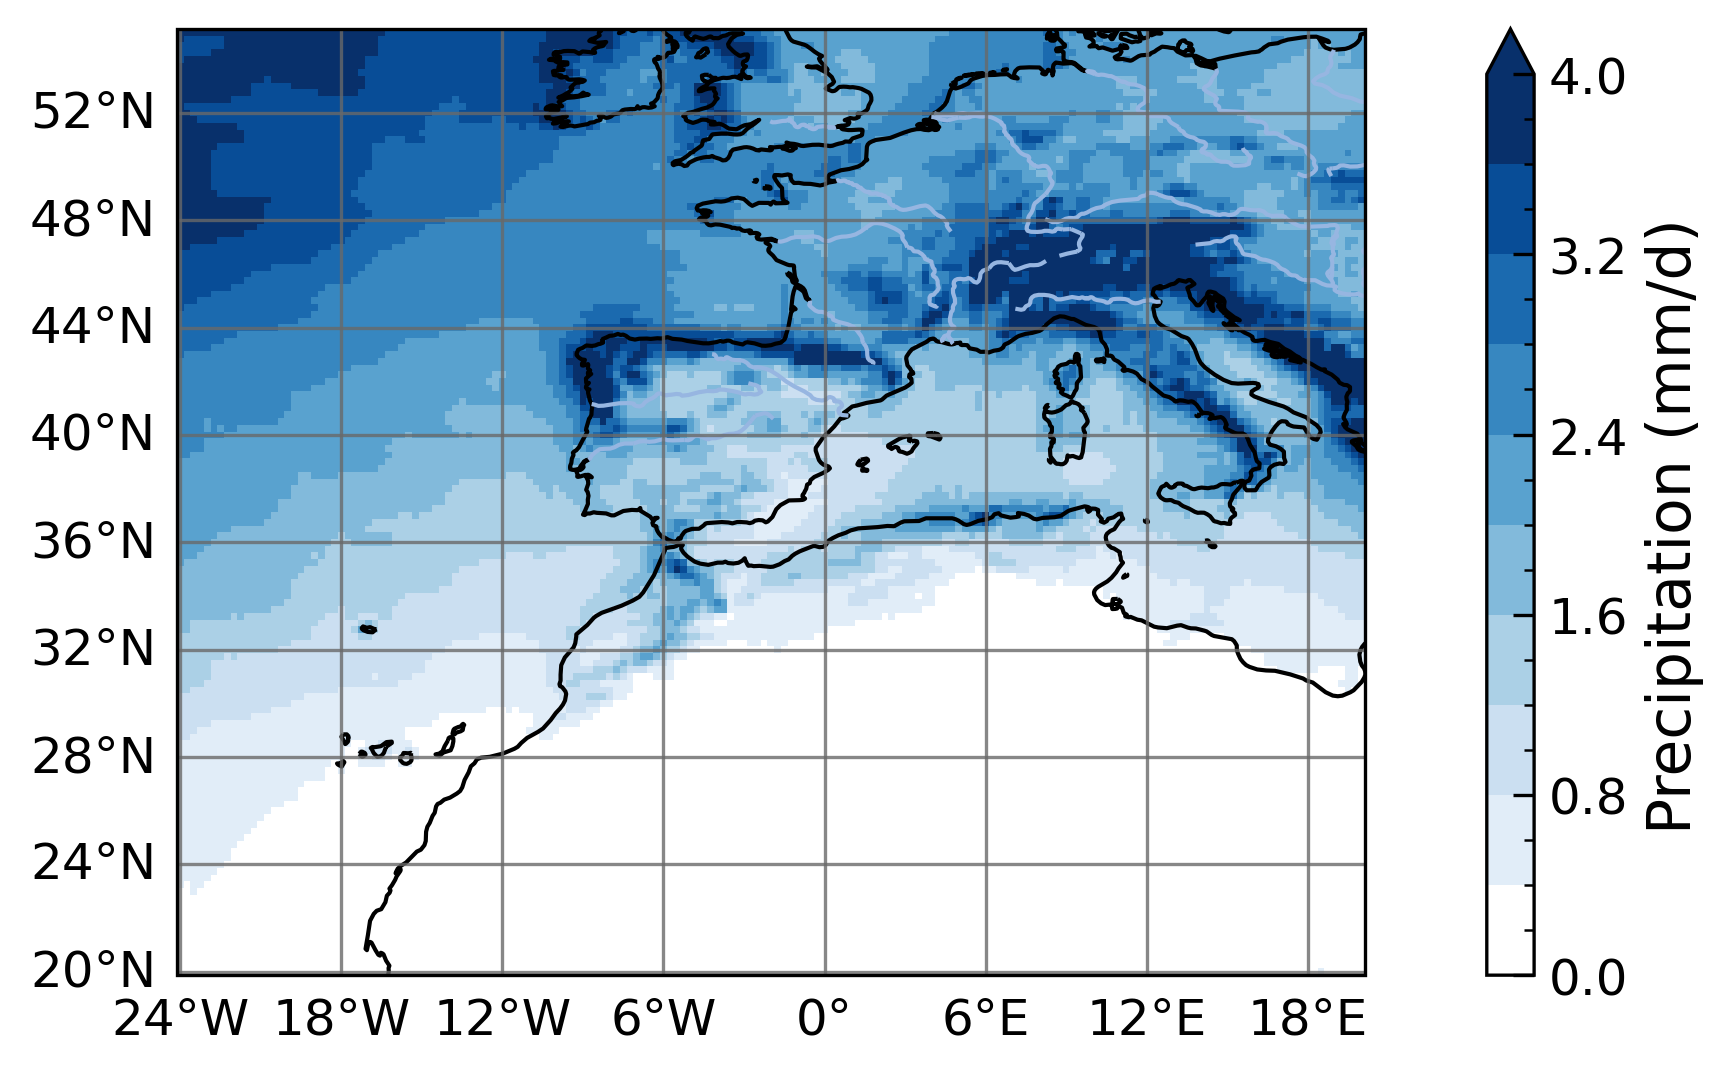
\includegraphics[width=\textwidth]{images/chap4/domain_size/var_map_precip_ERA5.png}
        \end{subfigure} &
        \begin{subfigure}[b]{0.33\textwidth}
            \caption{Downwelling shortwave \\radiation (W \persqm)}
            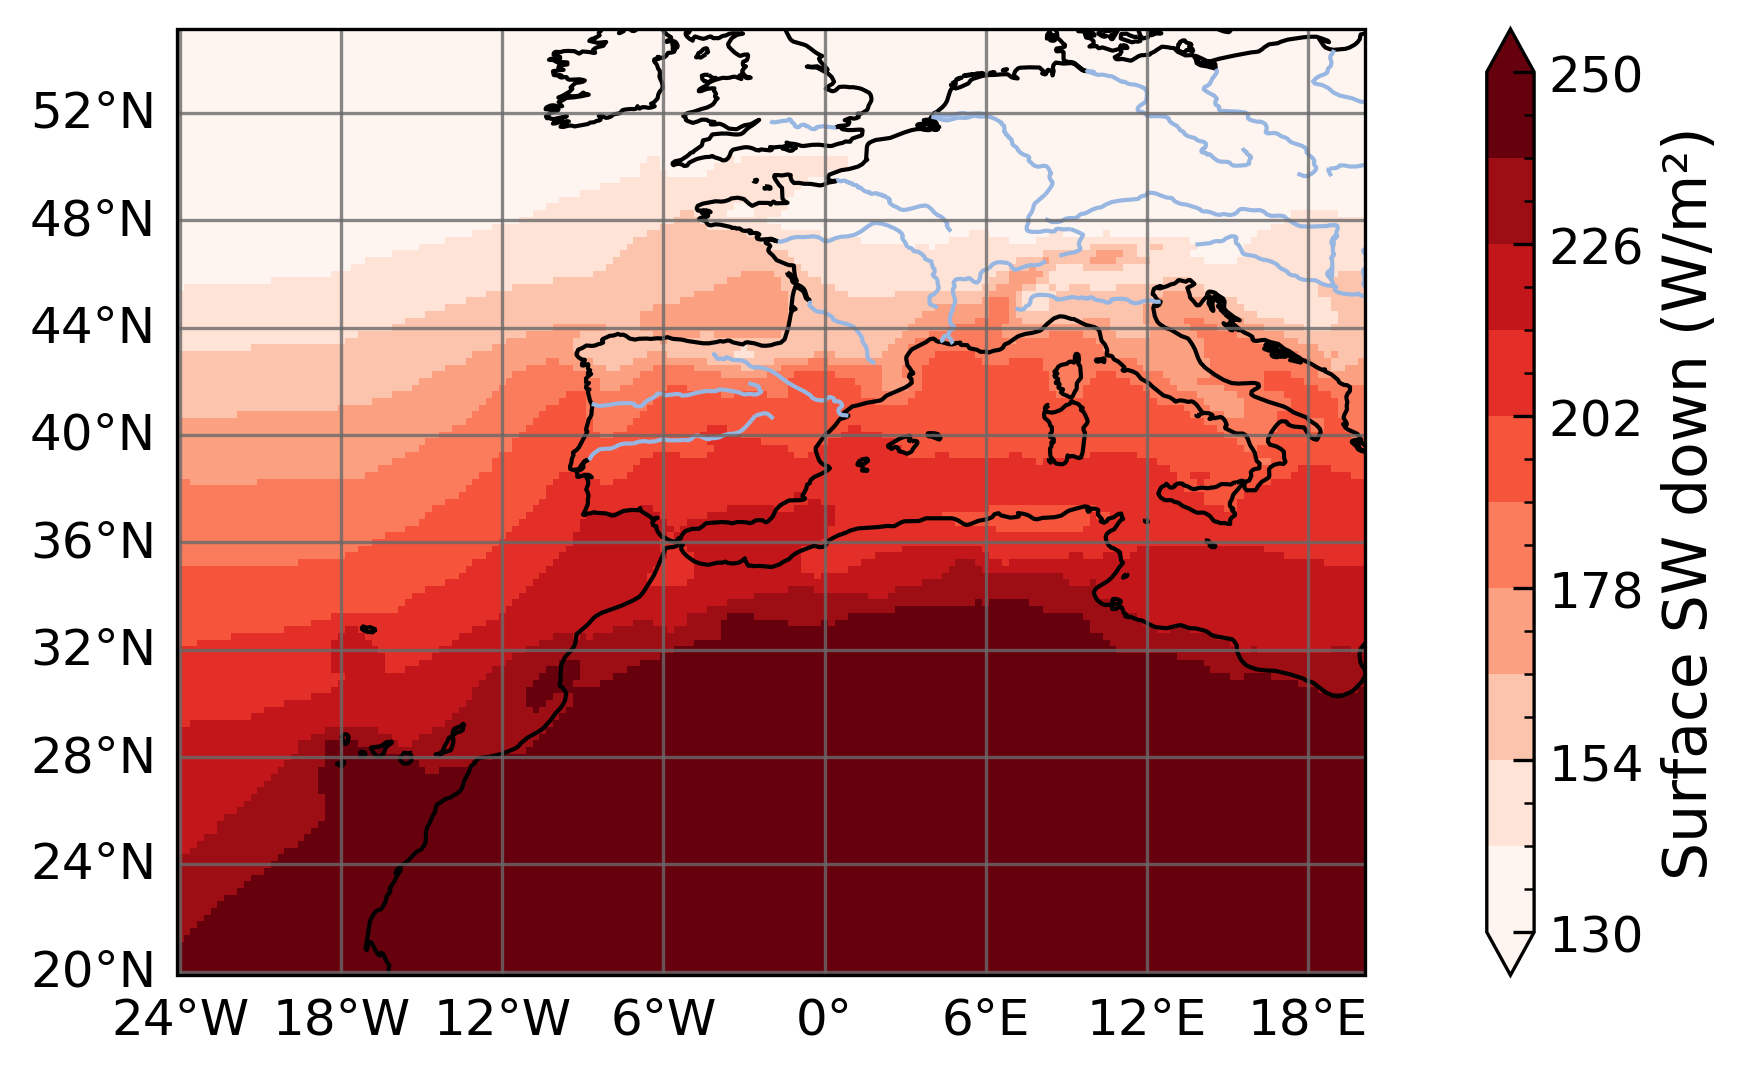
\includegraphics[width=\textwidth]{images/chap4/domain_size/var_map_SWdnSFC_ERA5.png}
        \end{subfigure} &
        \begin{subfigure}[b]{0.33\textwidth}
            \caption{Total cloud cover \\(cloud fraction in \%)}
            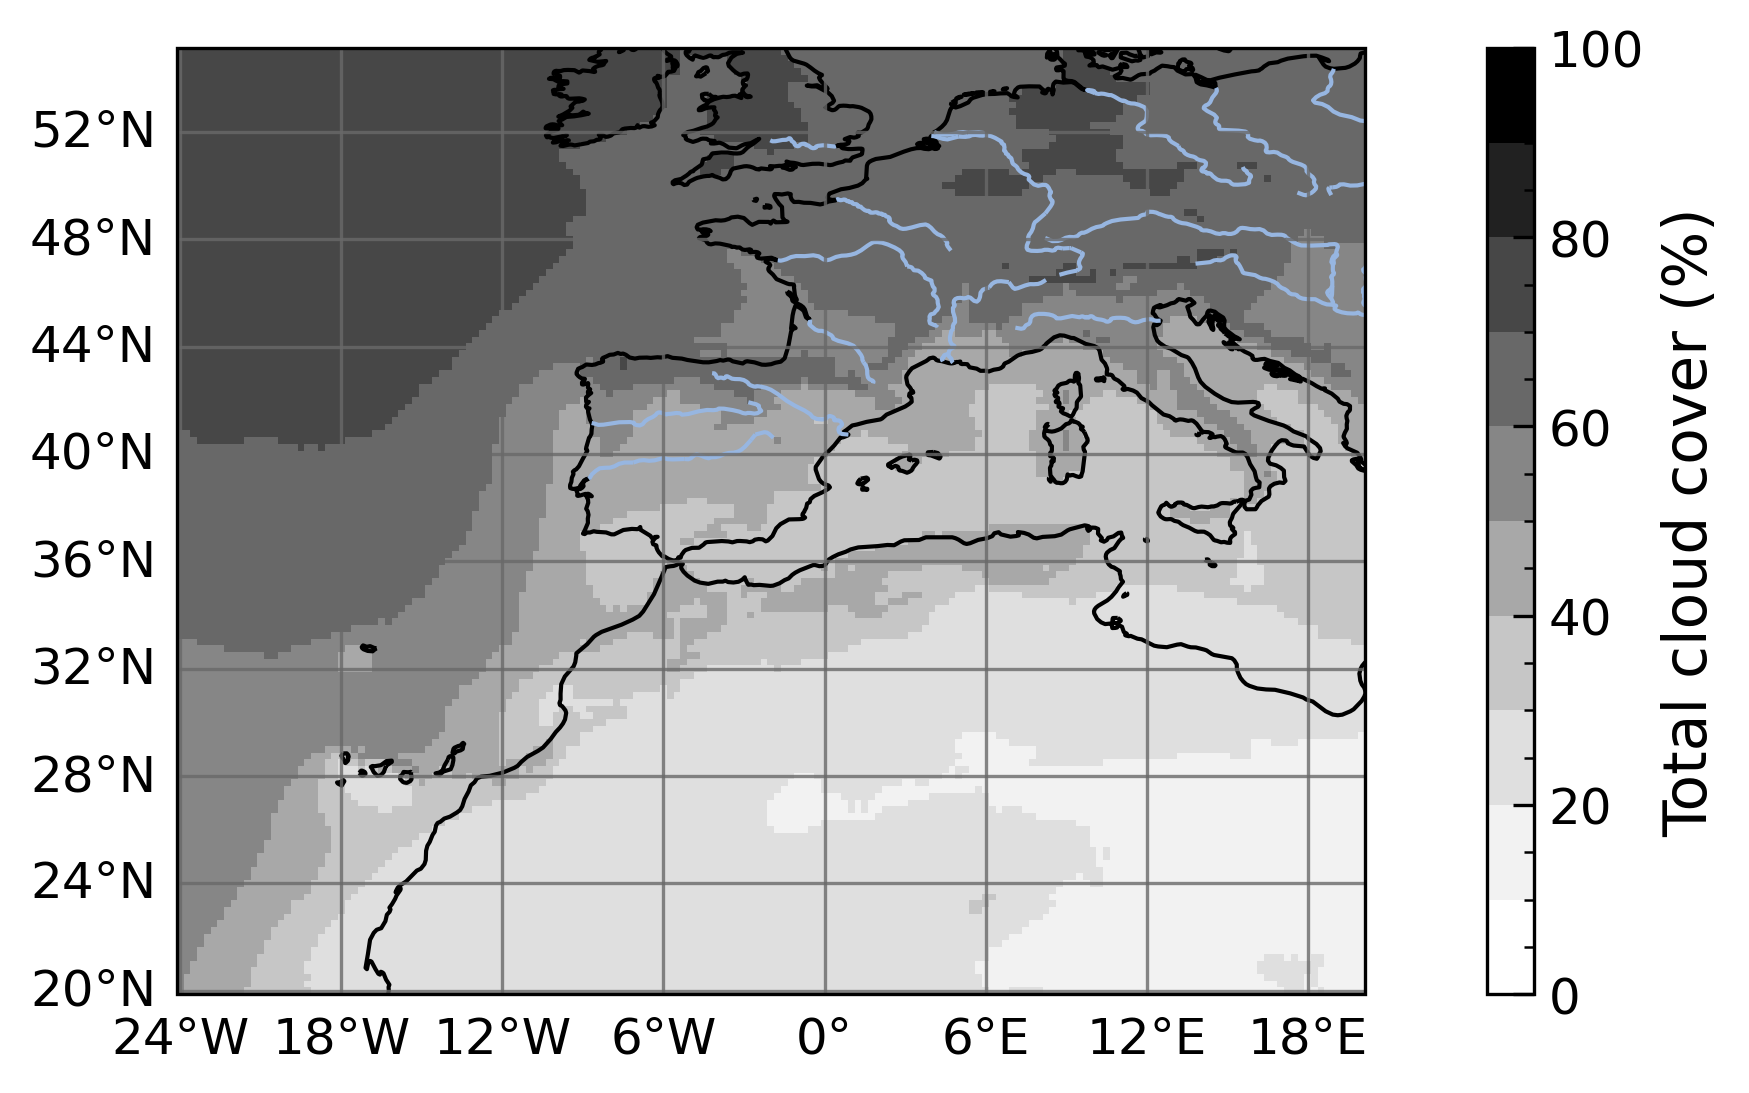
\includegraphics[width=\textwidth]{images/chap4/domain_size/var_map_cldt_ERA5.png}
        \end{subfigure} \\

        \begin{subfigure}[b]{0.33\textwidth}
            \caption{Evapotranspiration (mm \perday)}
            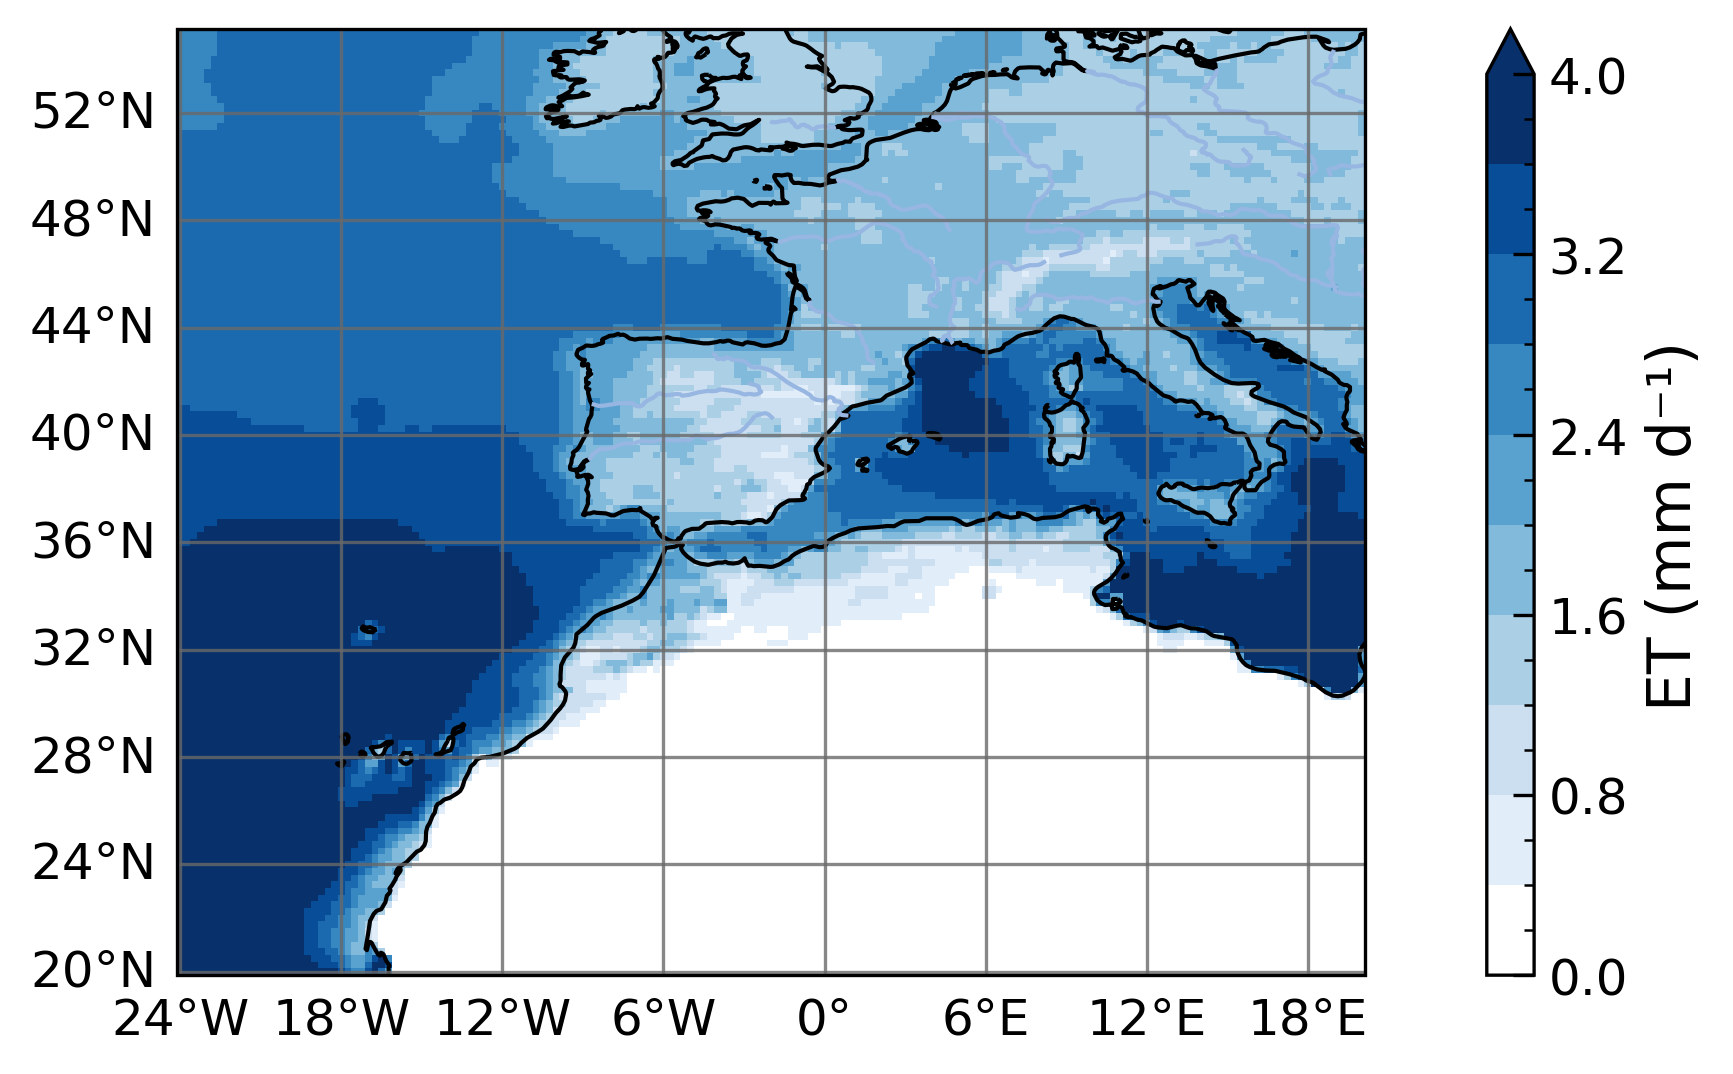
\includegraphics[width=\textwidth]{images/chap4/domain_size/var_map_evap_ERA5.png}
        \end{subfigure} &
        \begin{subfigure}[b]{0.33\textwidth}
            \caption{Downwelling longwave \\radiation (W \persqm)}
            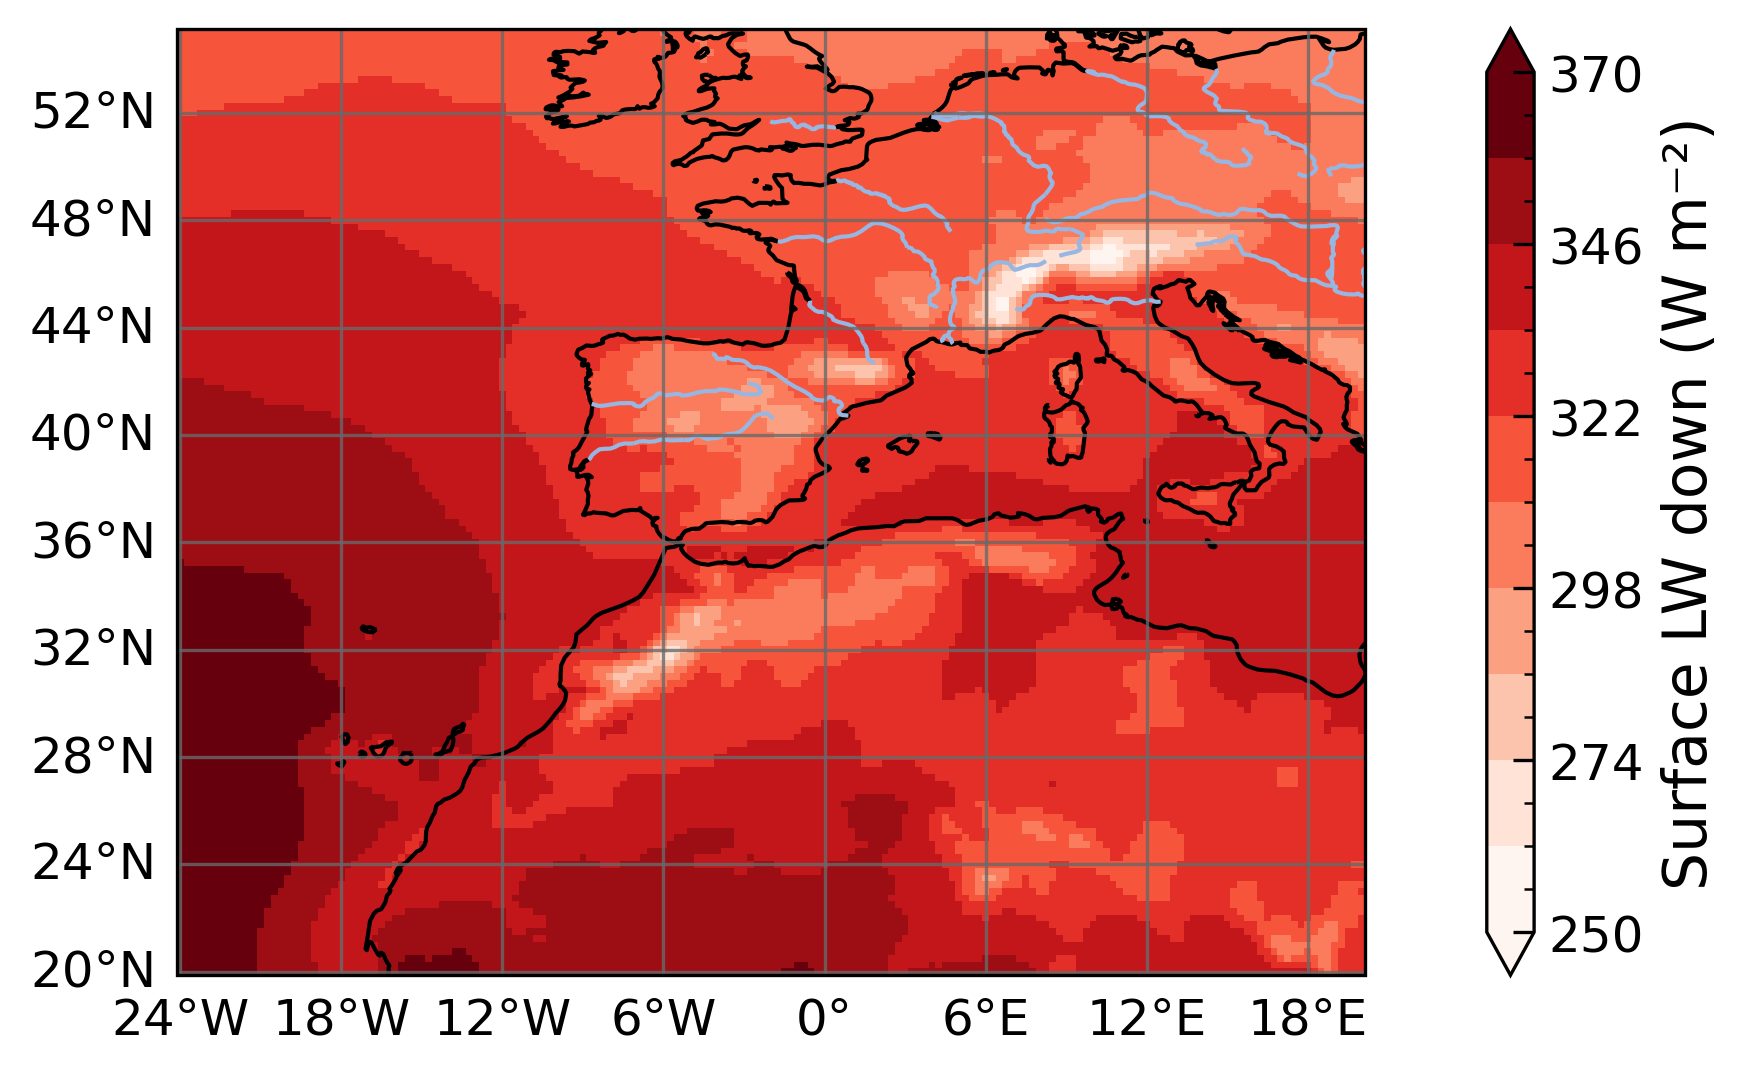
\includegraphics[width=\textwidth]{images/chap4/domain_size/var_map_LWdnSFC_ERA5.png}
        \end{subfigure} &
        \begin{subfigure}[b]{0.33\textwidth}
            \caption{Low cloud cover \\(cloud fraction in \%)}
            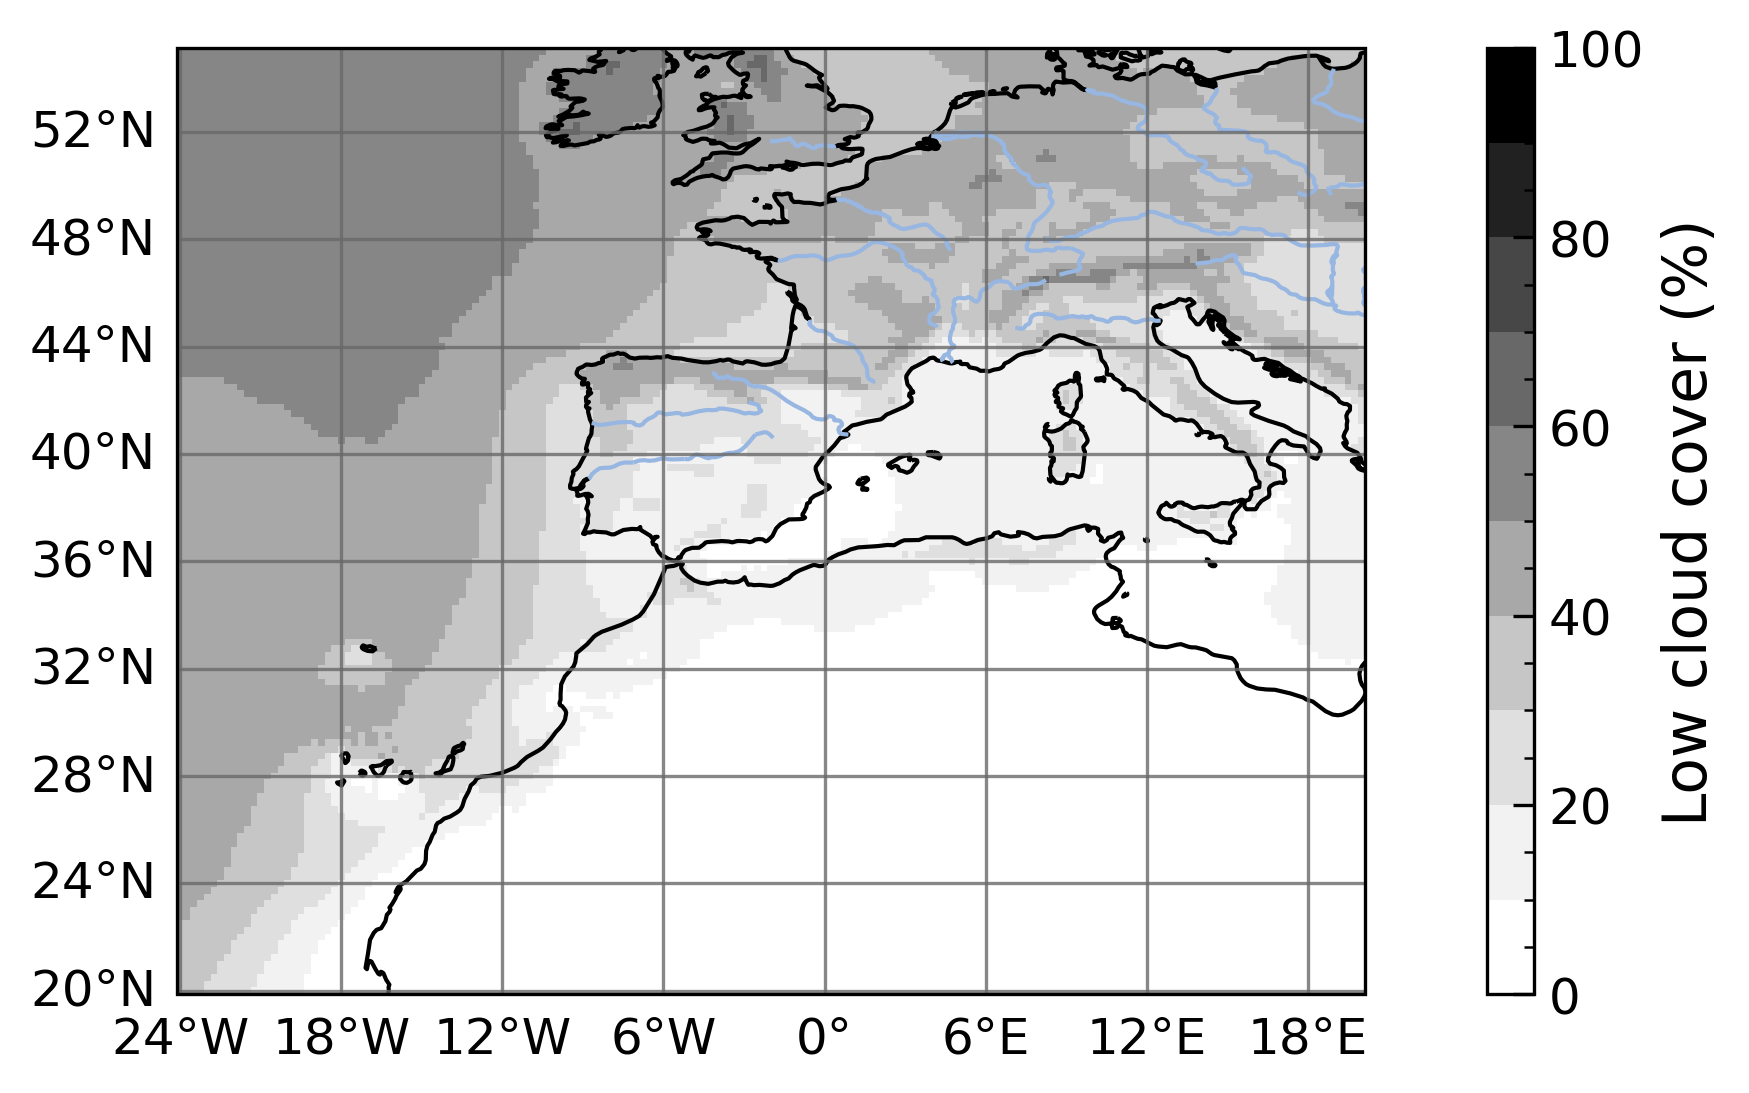
\includegraphics[width=\textwidth]{images/chap4/domain_size/var_map_cldl_ERA5.png}
        \end{subfigure}
    \end{tabular}
    \caption{Annual mean of the six variables of interest for the analysis of the LAM structural biases in ERA5 over the period 2010-2014.}
    \label{fig:ERA_var_maps}
\end{figure}
%todo:voir si meilleure mise en page des légendes est possible?

\section{Structural inconsistencies and influence of domain size}
\label{sec:domain_size}
The inconsistencies were identified with the initial simulation setup \smalld, by noticing that it presents little to no precipitation on the edges of the domain. The LAM displays a strong underestimation compared to ERA5 in the transition zone (Fig. \ref{fig:domain_size_P_ET_ERA_diff_maps}a), although it remains hard to determine if these biases have an influence on the rest of the domain. In particular,, the Iberian Peninsula exhibits underestimated precipitation along its northern and western coasts which might either be considered as the continuity of the bias on the edges, or as the consequence of other issues linked to rainfall at the transition between ocean and land.
This lack of precipitation is correlated to a lower ET on continents, which receive less water. However, over the Atlantic ocean and the Mediterranean sea, ET was surprisingly high, overestimating the values of ERA5 (Fig. \ref{fig:domain_size_P_ET_ERA_diff_maps}b). 

Simulations with the intermediate and large domains show that the strongest biases in precipitation are located in the transition zone, especially in the north-west of the domain which is not influenced by the presence of continents (Fig. \ref{fig:domain_size_P_ET_ERA_diff_maps}b-c).
In all simulations, the differences compared to ERA5 in the very edge of the domain correspond to a relative decrease between -80\% and -100\%, meaning the model computes almost no precipitation in these grid cells (Fig. \ref{fig:domain_size_ERA_reldiff_maps} in the appendix presents similar maps to Fig. \ref{fig:domain_size_P_ET_ERA_diff_maps} but with relative differences).
In the free zone, precipitation remains underestimated over the sea but much less than in \smalld, and the bias decreases towards the centre. Along the northern coast of the Peninsula, the underestimation is still present but seems structurally independent from the behaviour of the model on the edges of the domain.
The overestimation in ET is also confined to the northwestern edge of the domain and the large overestimation in the Mediterranean is reversed to an underestimation, of smaller magnitude, for both \interd and \larged (Fig. \ref{fig:domain_size_P_ET_ERA_diff_maps}e-f).
As mentioned before, although ERA5 cannot be considered as the best reference product for all the variables considered, it is the spatial structure of the biases that is striking here, since they are independent of the structure of the variable (Fig. \ref{fig:ERA_var_maps}), and follow the edges of the domain even when the radius changes.

%figure : maps of diff vs ERA for 3 domain sizes : precip, evap
\begin{figure}[htbp]
    \centering
    \begin{tabular}{ccc}
        %precip
        \begin{subfigure}[b]{0.33\textwidth}
            \caption{Precipitation bias to ERA5\\(mm \perday, \smalld)}
            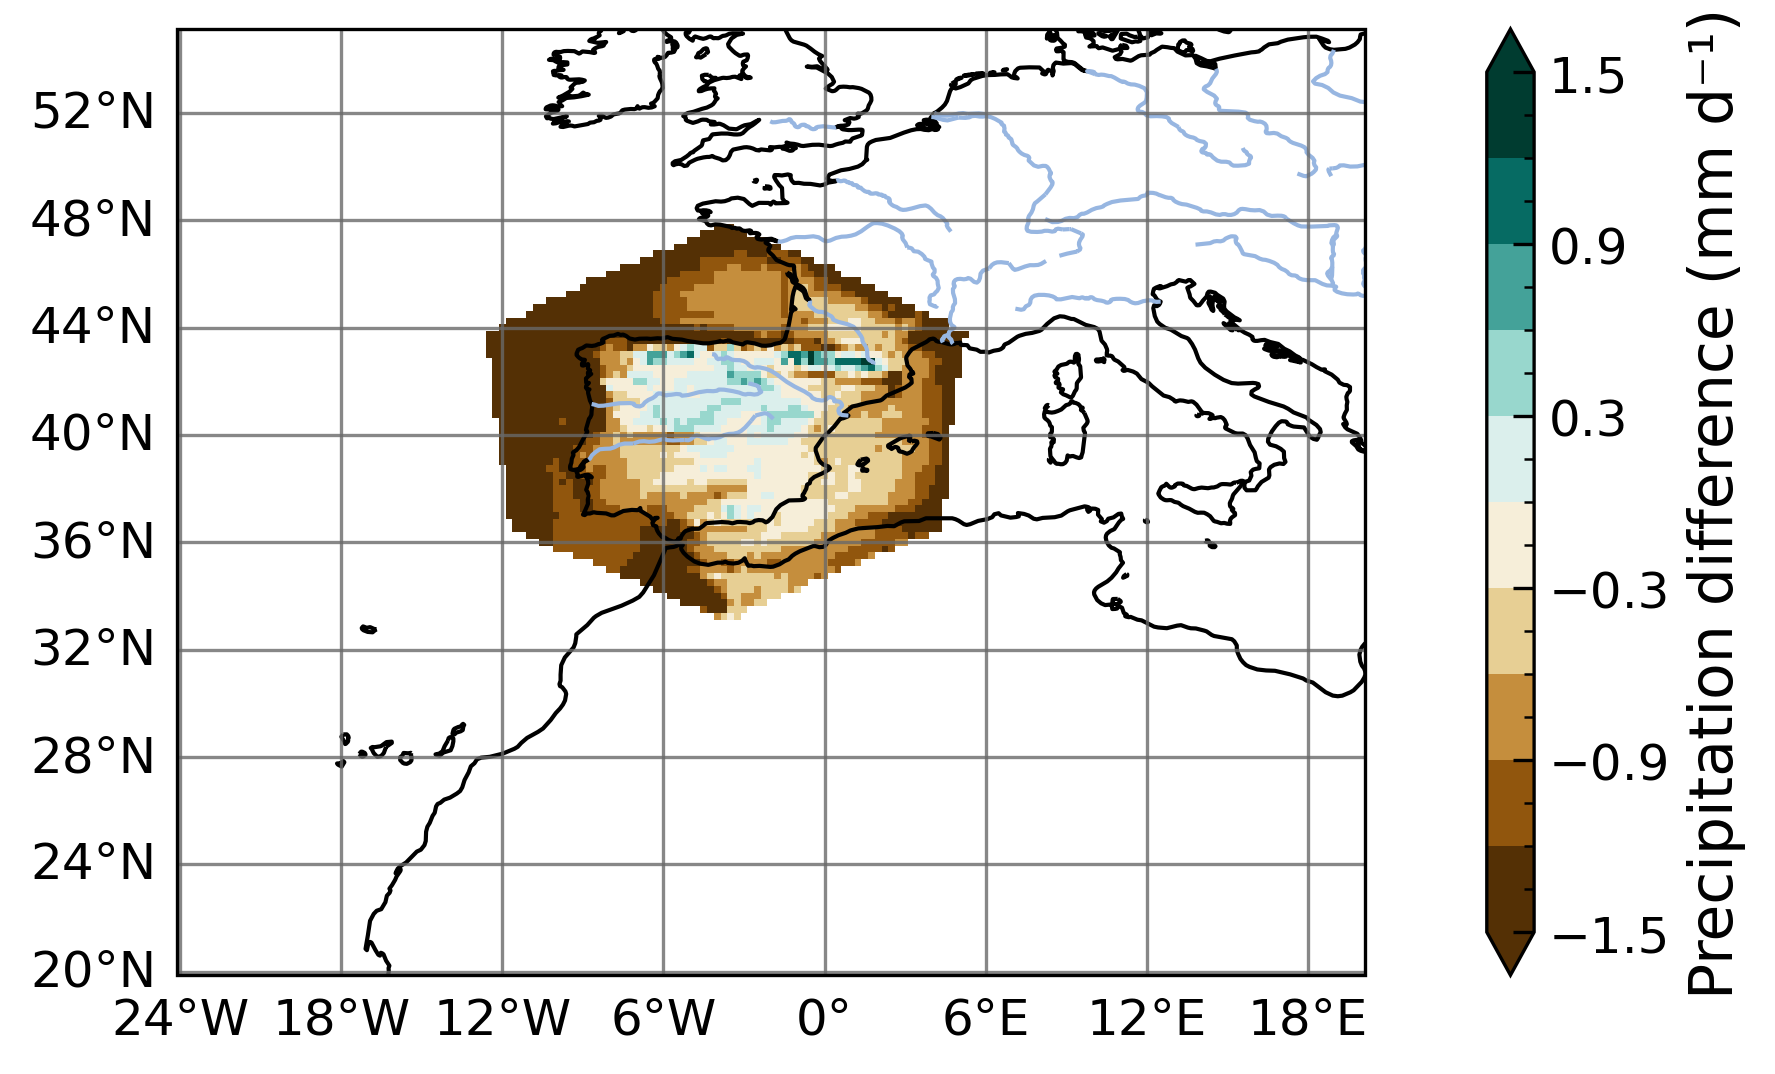
\includegraphics[width=\textwidth]{images/chap4/domain_size/diff_map_precip_era_LAM_1000km_NBP40.png}
        \end{subfigure} &
        \begin{subfigure}[b]{0.33\textwidth}
            \caption{Precipitation bias to ERA5\\(mm \perday, \interd)}
            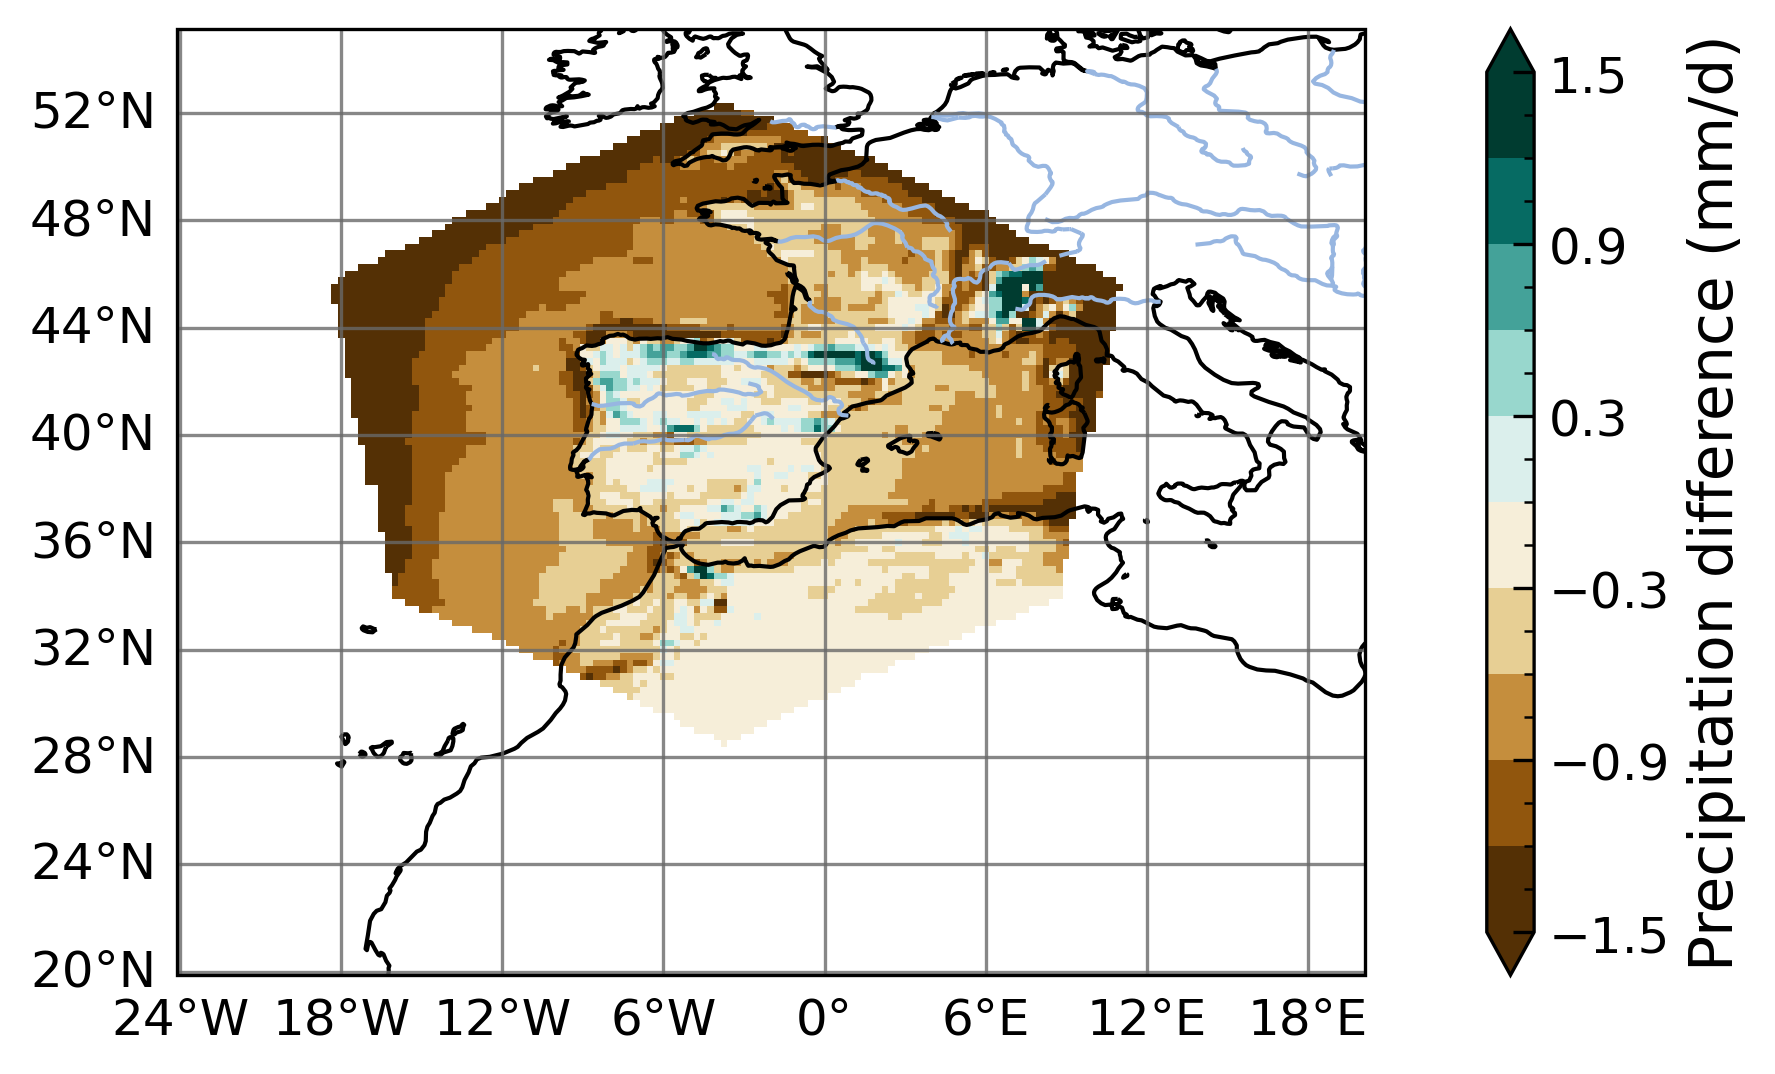
\includegraphics[width=\textwidth]{images/chap4/domain_size/diff_map_precip_era_LAM_1500km_NBP60.png}
        \end{subfigure} &
        \begin{subfigure}[b]{0.33\textwidth}
            \caption{Precipitation bias to ERA5 \\(mm \perday, \larged)}
            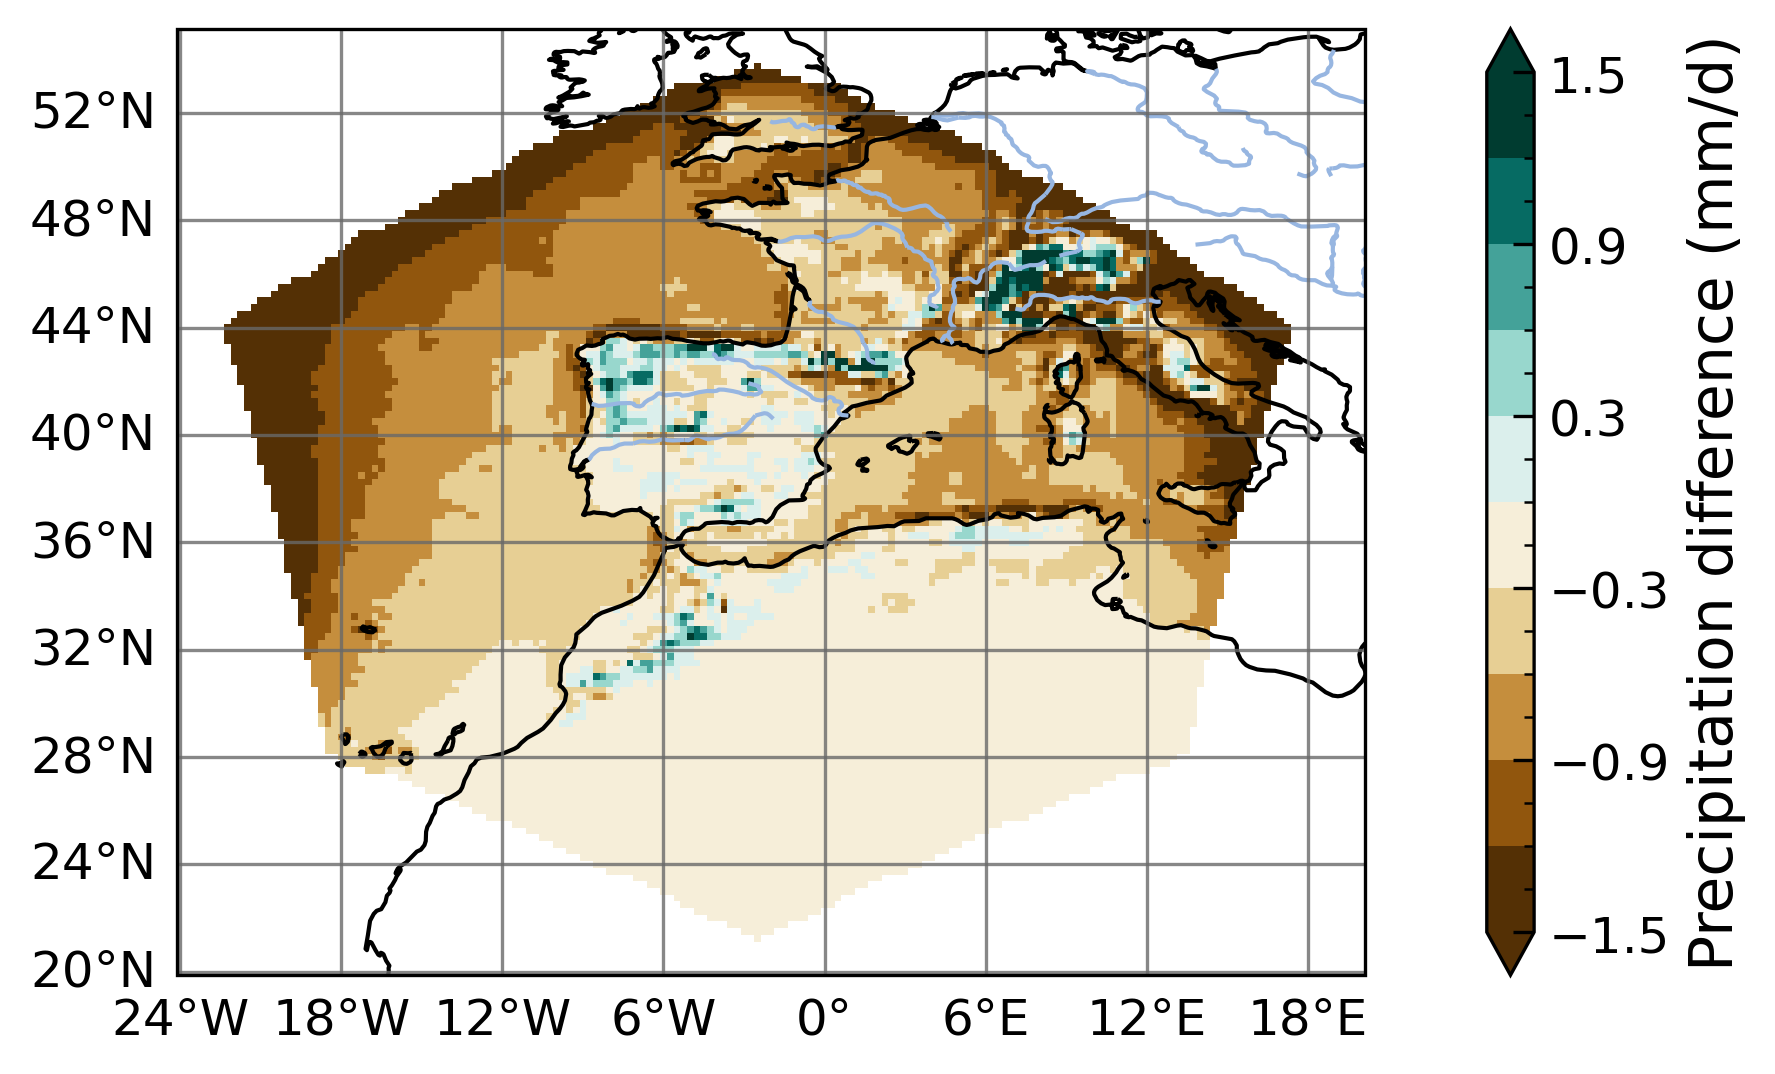
\includegraphics[width=\textwidth]{images/chap4/domain_size/diff_map_precip_era_LAM_2000km_NBP80.png}
        \end{subfigure} \\
        
        %evap
        \begin{subfigure}[b]{0.33\textwidth}
            \caption{ET bias to ERA5\\(mm \perday, \smalld)}
            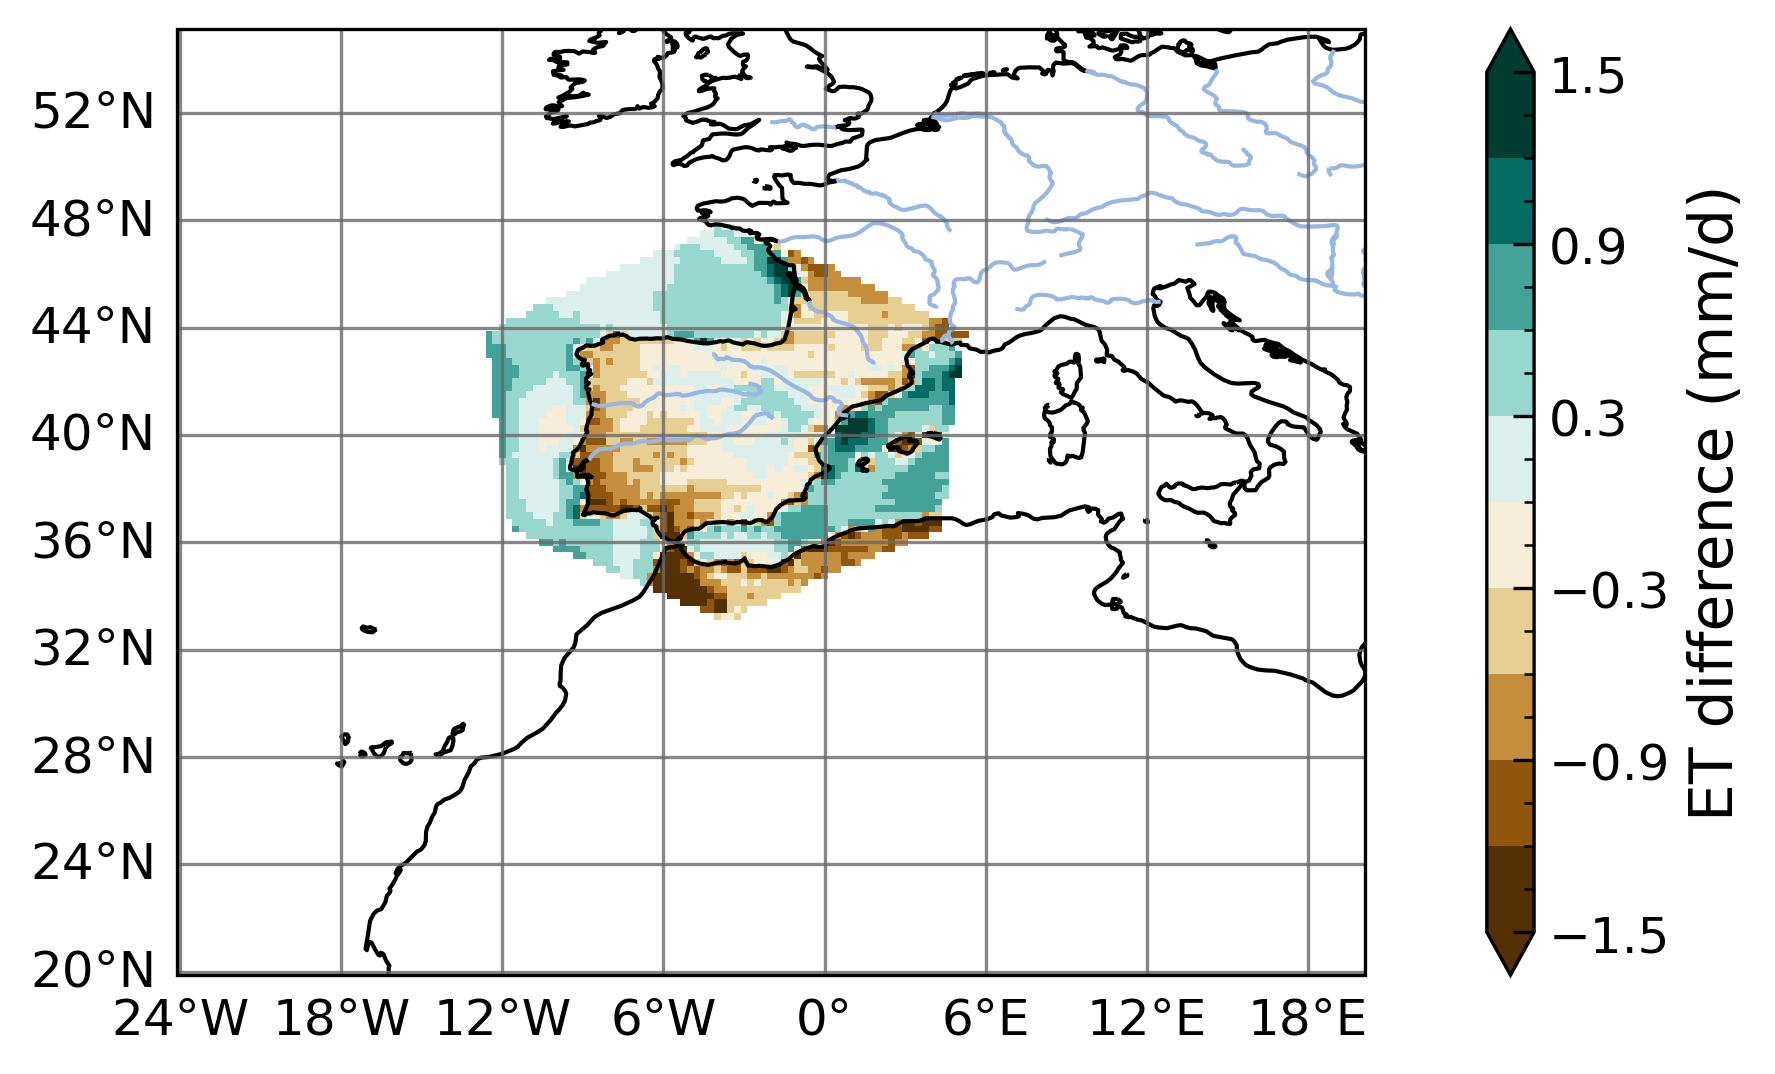
\includegraphics[width=\textwidth]{images/chap4/domain_size/diff_map_evap_era_LAM_1000km_NBP40.png}
        \end{subfigure} &
        \begin{subfigure}[b]{0.33\textwidth}
            \caption{ET bias to ERA5\\(mm \perday, \interd)}
            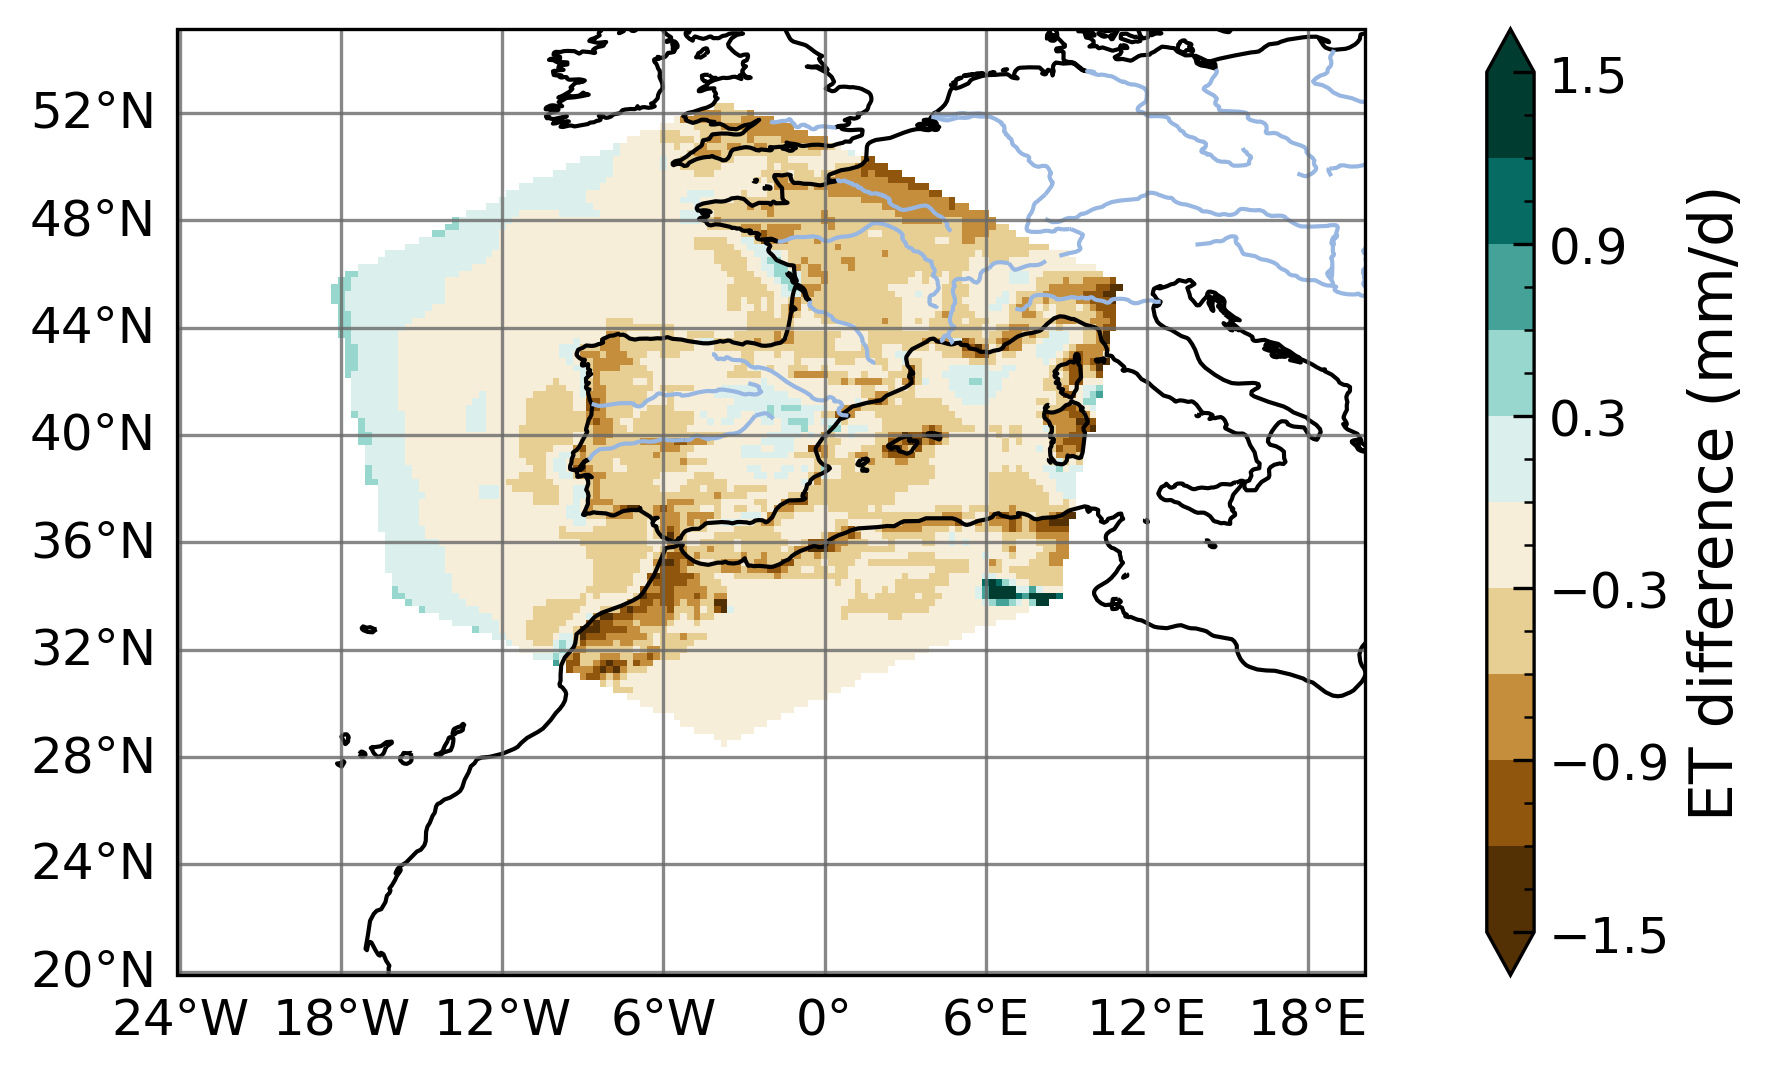
\includegraphics[width=\textwidth]{images/chap4/domain_size/diff_map_evap_era_LAM_1500km_NBP60.png}
        \end{subfigure} &
        \begin{subfigure}[b]{0.33\textwidth}
            \caption{ET bias to ERA5\\(mm \perday, \larged)}
            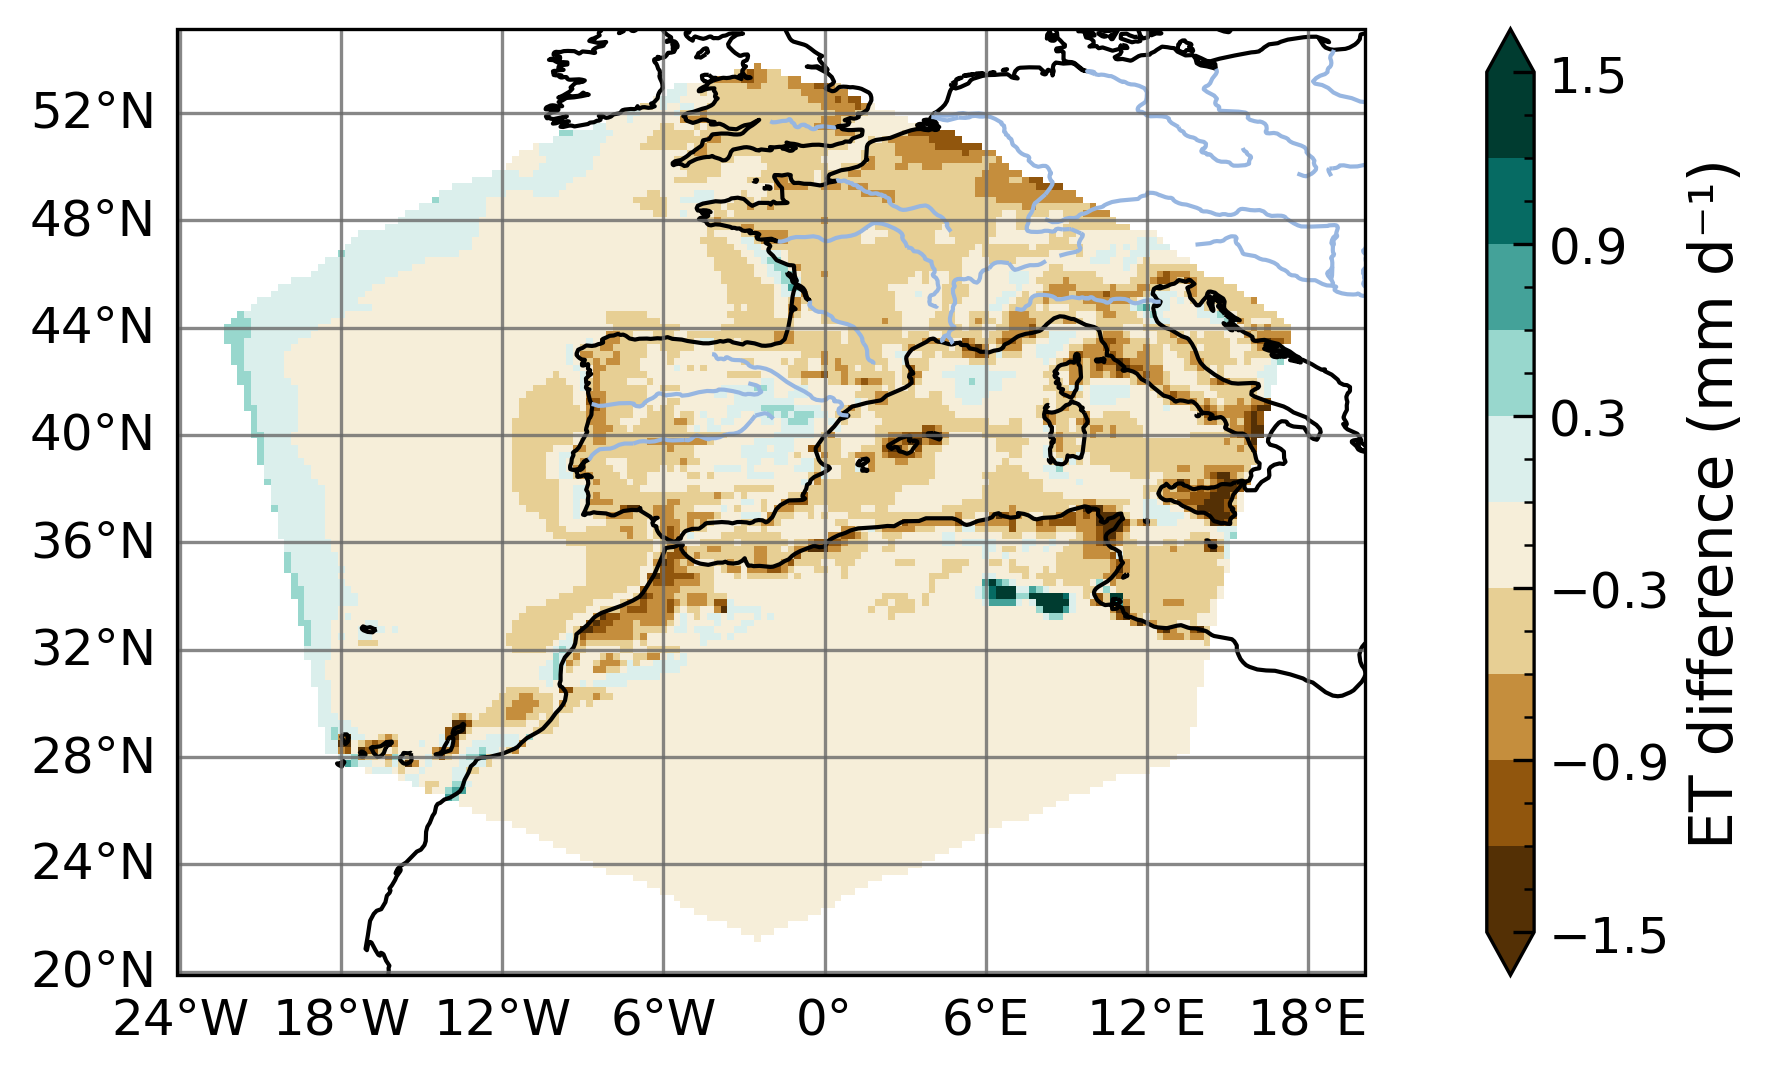
\includegraphics[width=\textwidth]{images/chap4/domain_size/diff_map_evap_era_LAM_2000km_NBP80.png}
        \end{subfigure} 
    \end{tabular}
    \caption{Precipitation (a-c) and evapotranspiration (d-f) biases compared to ERA5 over 2010-2014 for three simulations with small, intermediate and large domain sizes.}
    \label{fig:domain_size_P_ET_ERA_diff_maps}
\end{figure}

These first findings led to the hypothesis that the physics of the LAM is not behaving in a normal way in the transition zone, and more specifically the large-scale water condensation scheme. 
Comparisons with ERA5 show an underestimation of total cloud cover in the transition zone (Fig. \ref{fig:domain_size_clouds_ERA_diff_maps}a-c) and particularly of low cloud cover (Fig. \ref{fig:domain_size_clouds_ERA_diff_maps}d-f), which constitutes its most important component (Fig. \ref{fig:ERA_var_maps}c, f). %option (commentaire FC: profil moyen de nuage ou sur 1 ou 2 points de l'atlantique)
The absence of clouds allows more solar radiation to reach the surface, leading to higher values of the downwelling shortwave radiation flux (Fig. \ref{fig:domain_size_clouds_ERA_diff_maps}g-i). This can explain the higher ET values since it provides more available energy for evaporation of seawater.
Having less condensed water also leads to a smaller downwelling longwave radiation flux in the transition zone (Fig. \ref{fig:domain_size_clouds_ERA_diff_maps}j-l). This relationship is further illustrated in the central part of the domain, where the downwelling longwave radiation flux and low cloud cover are both overestimated, following similar spatial patterns.

%figure : maps of diff vs ERA for 3 domain sizes : SW, LW, cloud cover
\begin{figure}[htbp]
    \centering
    \begin{tabular}{ccc}
        %total
        \begin{subfigure}[b]{0.33\textwidth}
            \caption{Total cloud cover bias\\(\%, \smalld)}
            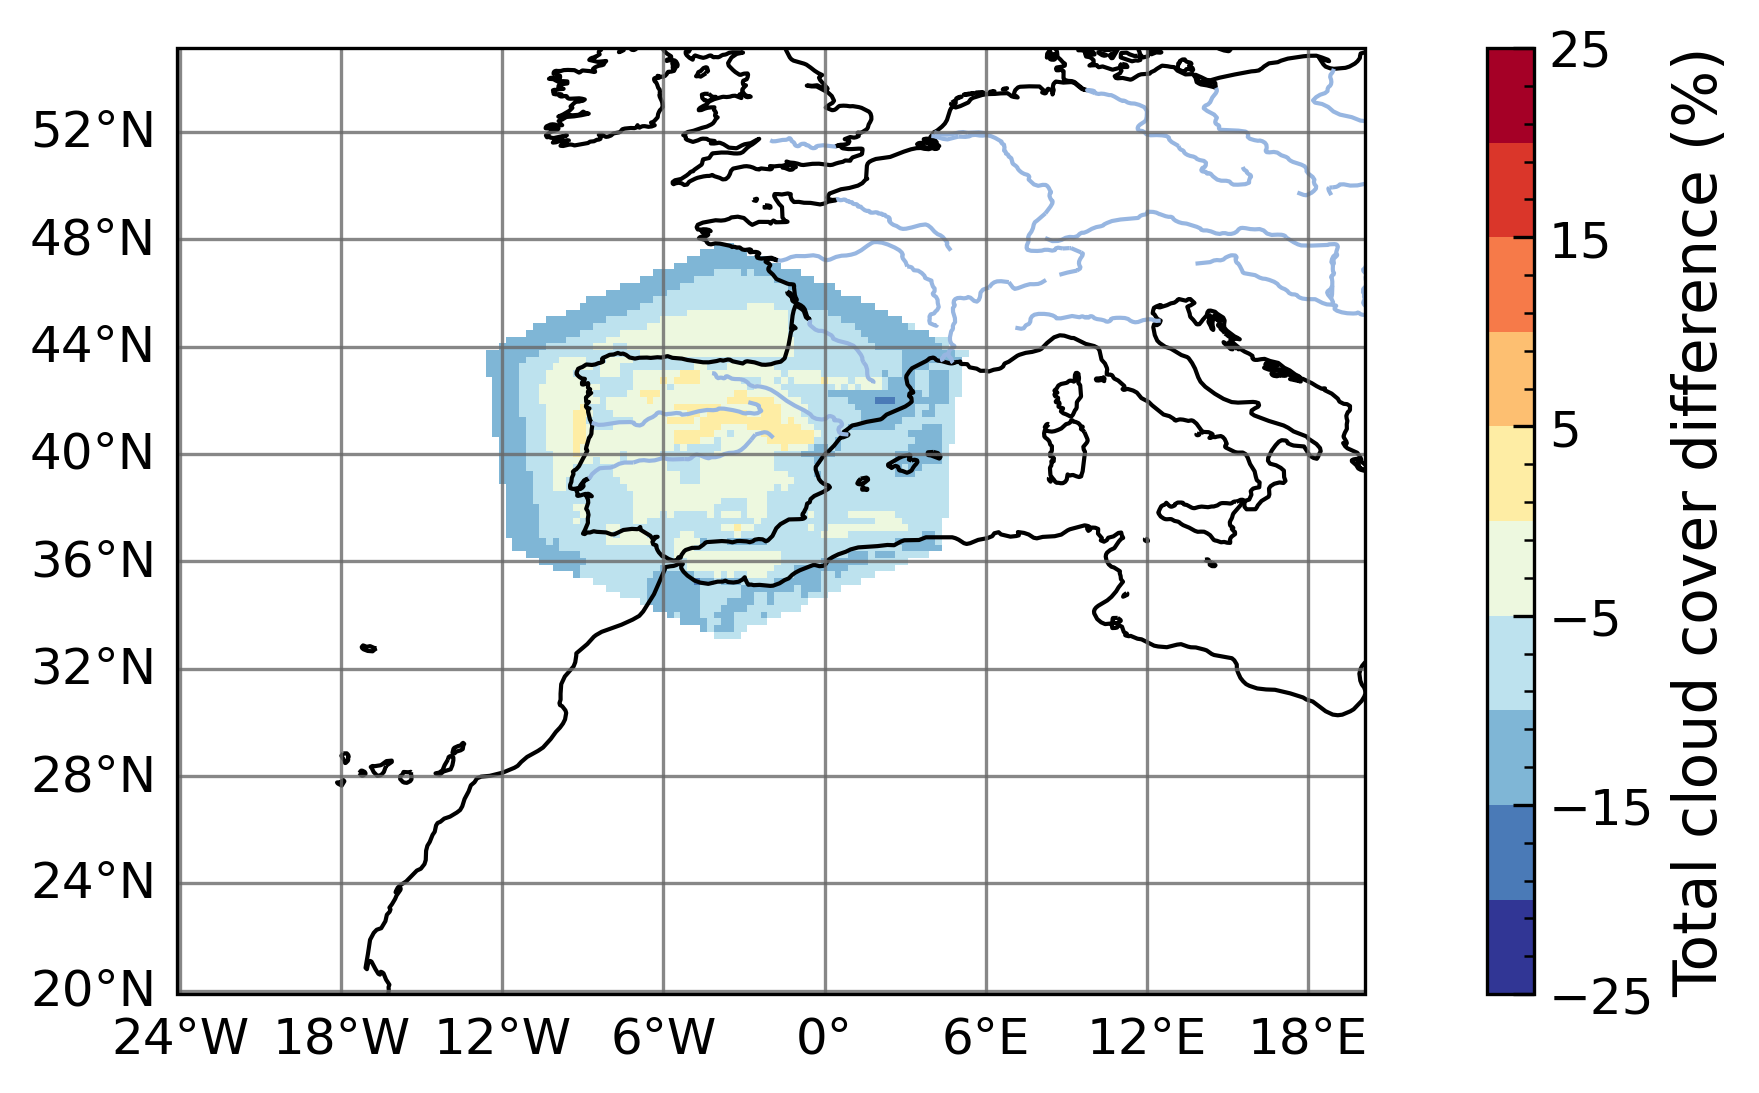
\includegraphics[width=\textwidth]{images/chap4/domain_size/diff_map_cldt_era_LAM_1000km_NBP40.png}
        \end{subfigure} &
        \begin{subfigure}[b]{0.33\textwidth}
            \caption{Total cloud cover bias\\(\%, \interd)}
            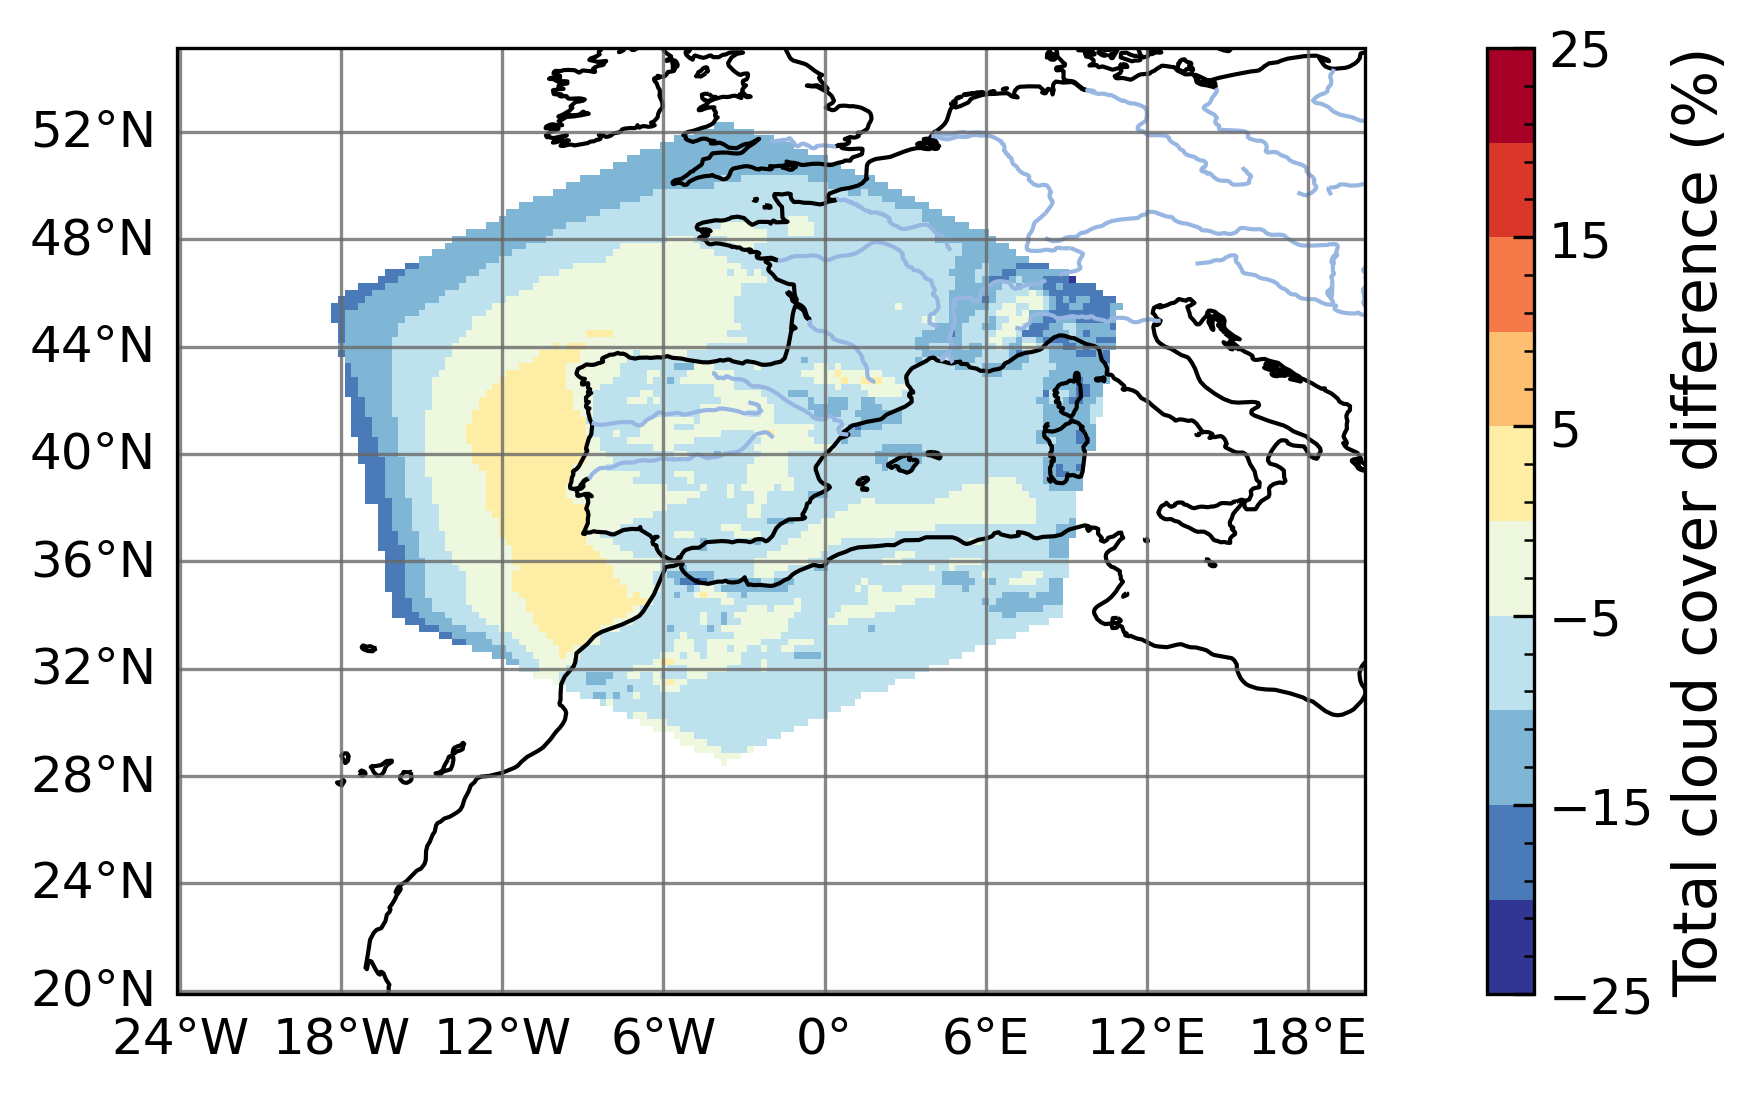
\includegraphics[width=\textwidth]{images/chap4/domain_size/diff_map_cldt_era_LAM_1500km_NBP60.png}
        \end{subfigure} &
        \begin{subfigure}[b]{0.33\textwidth}
            \caption{Total cloud cover bias\\(\%, \larged)}
            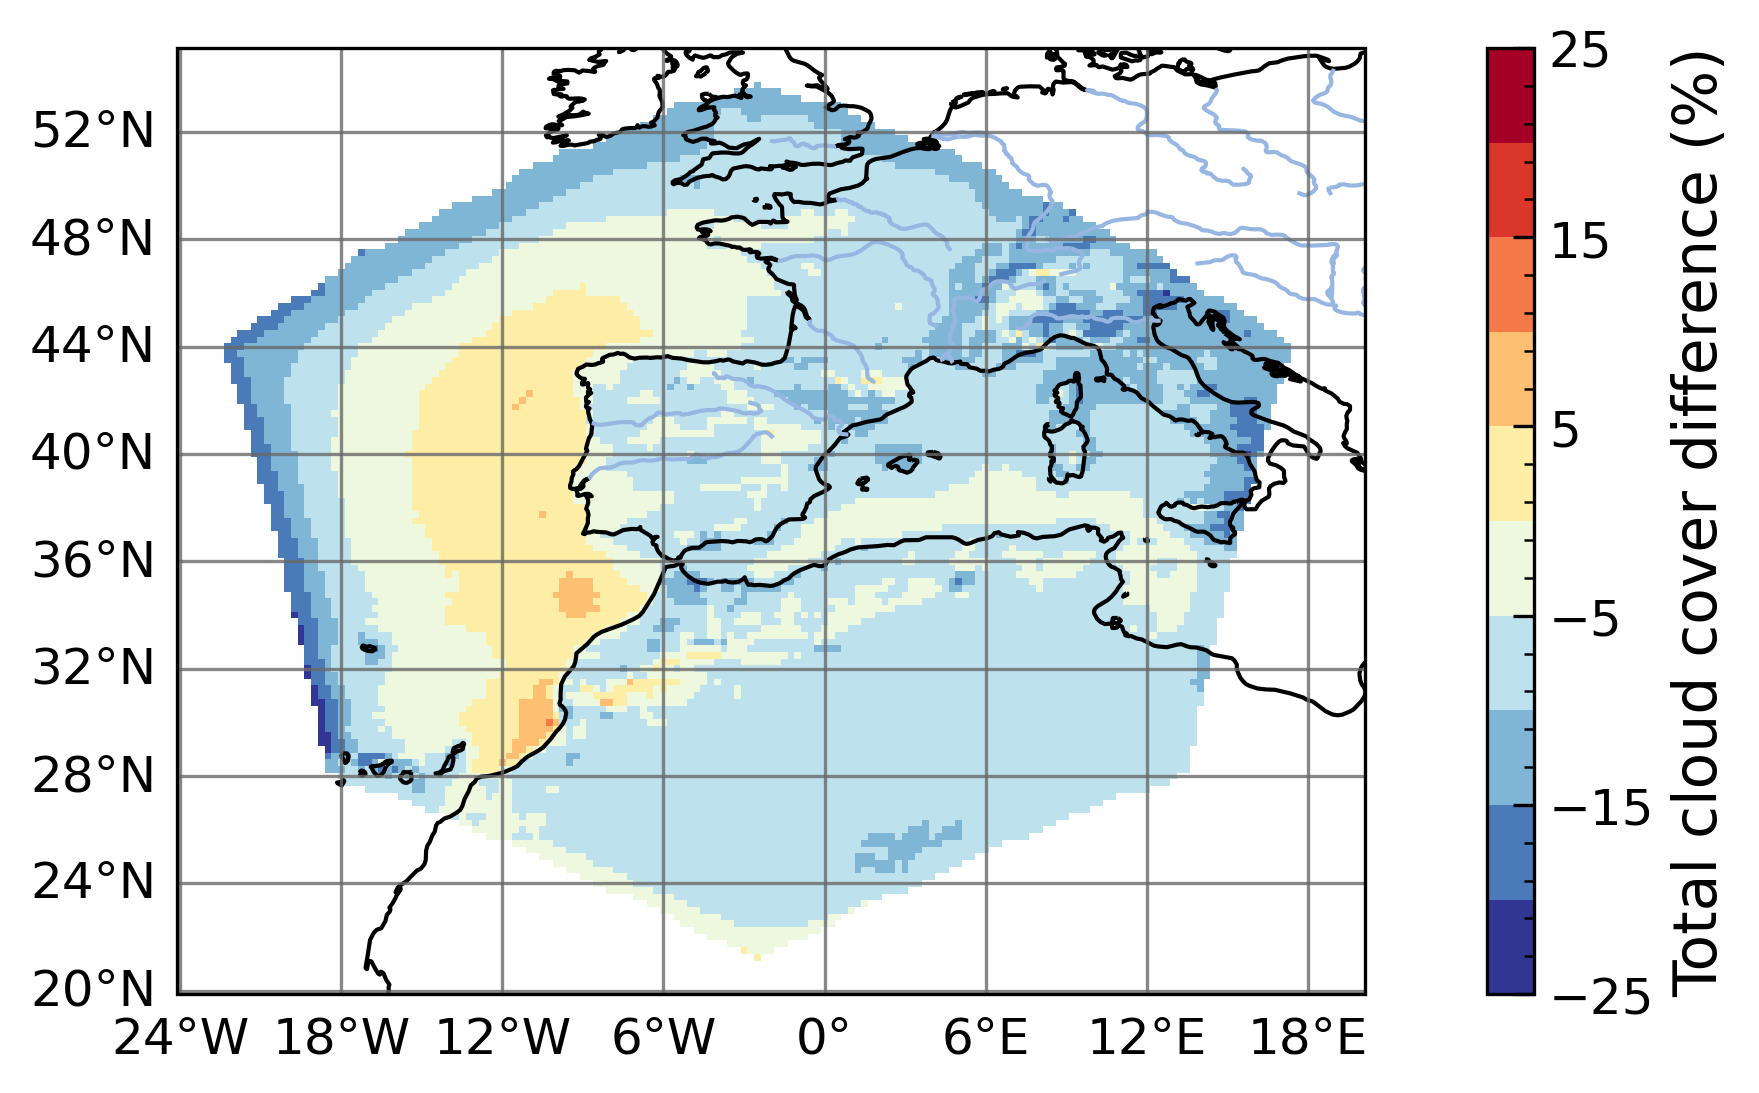
\includegraphics[width=\textwidth]{images/chap4/domain_size/diff_map_cldt_era_LAM_2000km_NBP80.png}
        \end{subfigure} \\
        
        %low
        \begin{subfigure}[b]{0.33\textwidth}
            \caption{Low cloud cover bias\\(\%, \smalld)}
            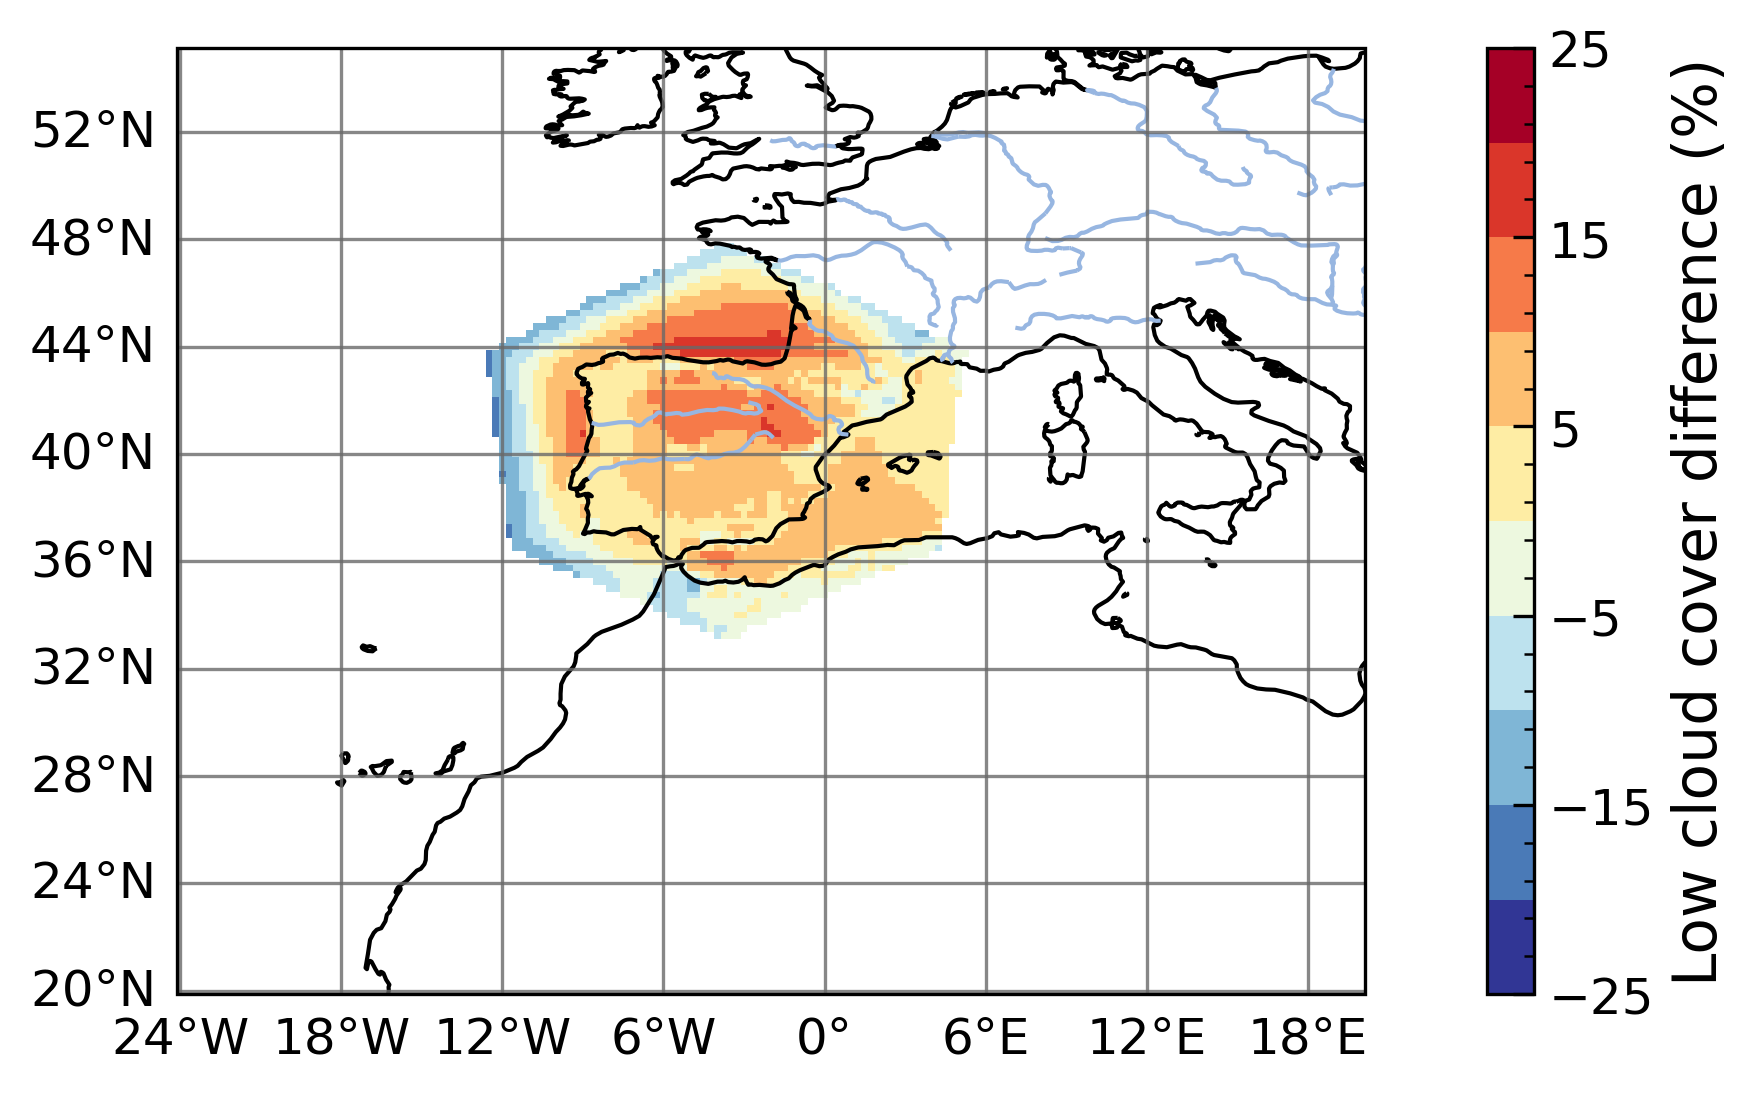
\includegraphics[width=\textwidth]{images/chap4/domain_size/diff_map_cldl_era_LAM_1000km_NBP40.png}
        \end{subfigure} &
        \begin{subfigure}[b]{0.33\textwidth}
            \caption{Low cloud cover bias\\(\%, \interd)}
            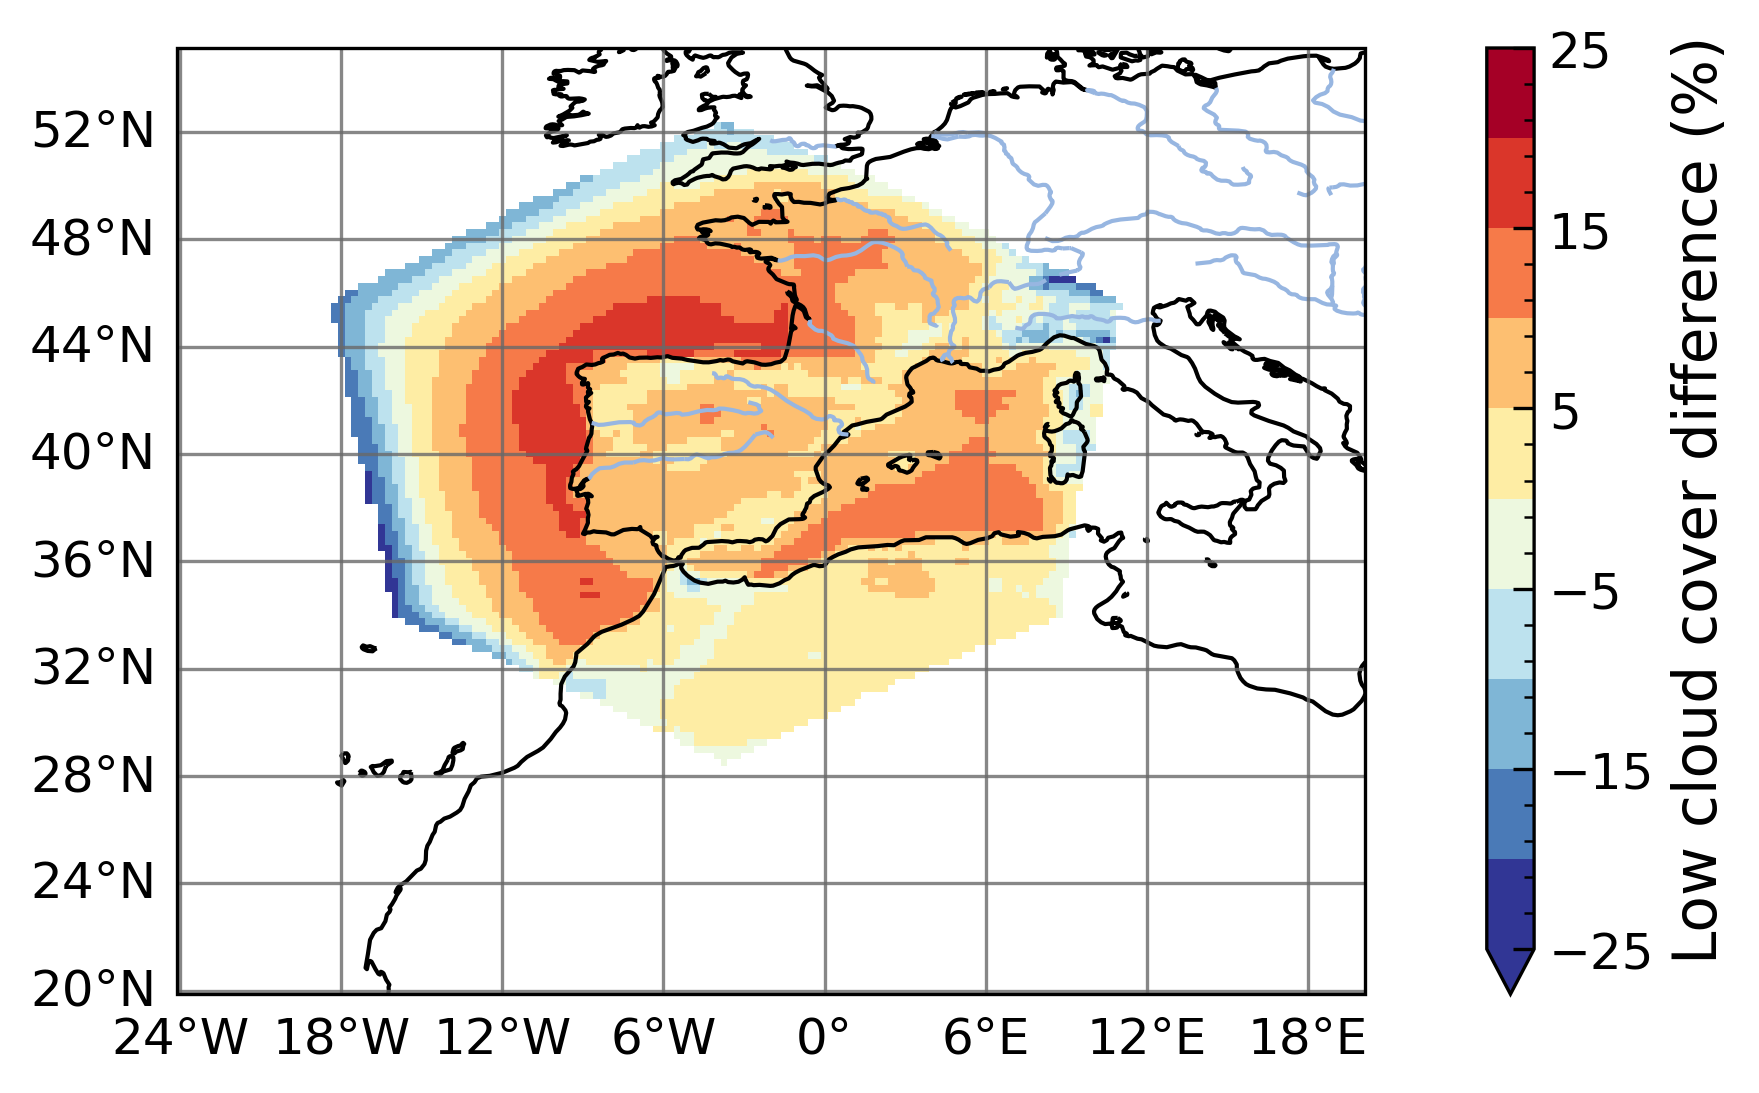
\includegraphics[width=\textwidth]{images/chap4/domain_size/diff_map_cldl_era_LAM_1500km_NBP60.png}
        \end{subfigure} &
        \begin{subfigure}[b]{0.33\textwidth}
            \caption{Low cloud cover bias\\(\%, \larged)}
            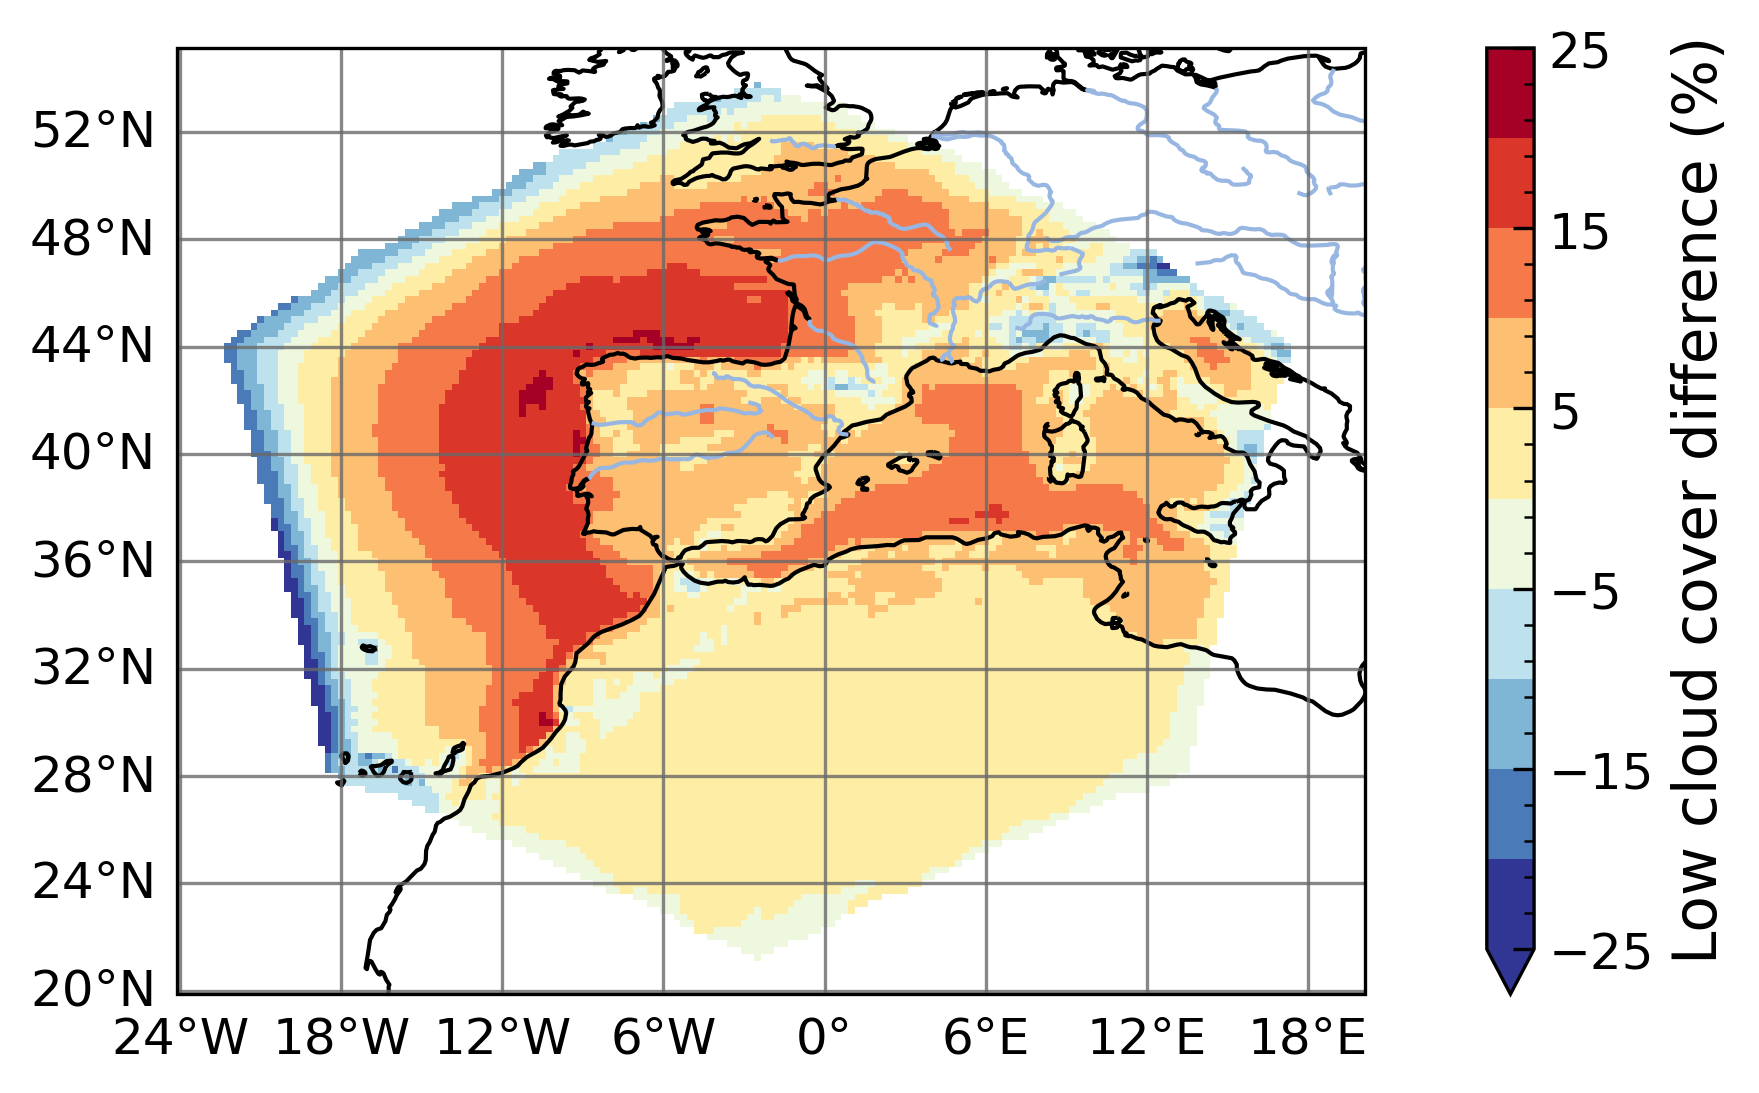
\includegraphics[width=\textwidth]{images/chap4/domain_size/diff_map_cldl_era_LAM_2000km_NBP80.png}
        \end{subfigure} \\

        %SWdn
        \begin{subfigure}[b]{0.33\textwidth}
            \caption{Downwelling SW flux bias\\(W \persqm, \smalld)}
            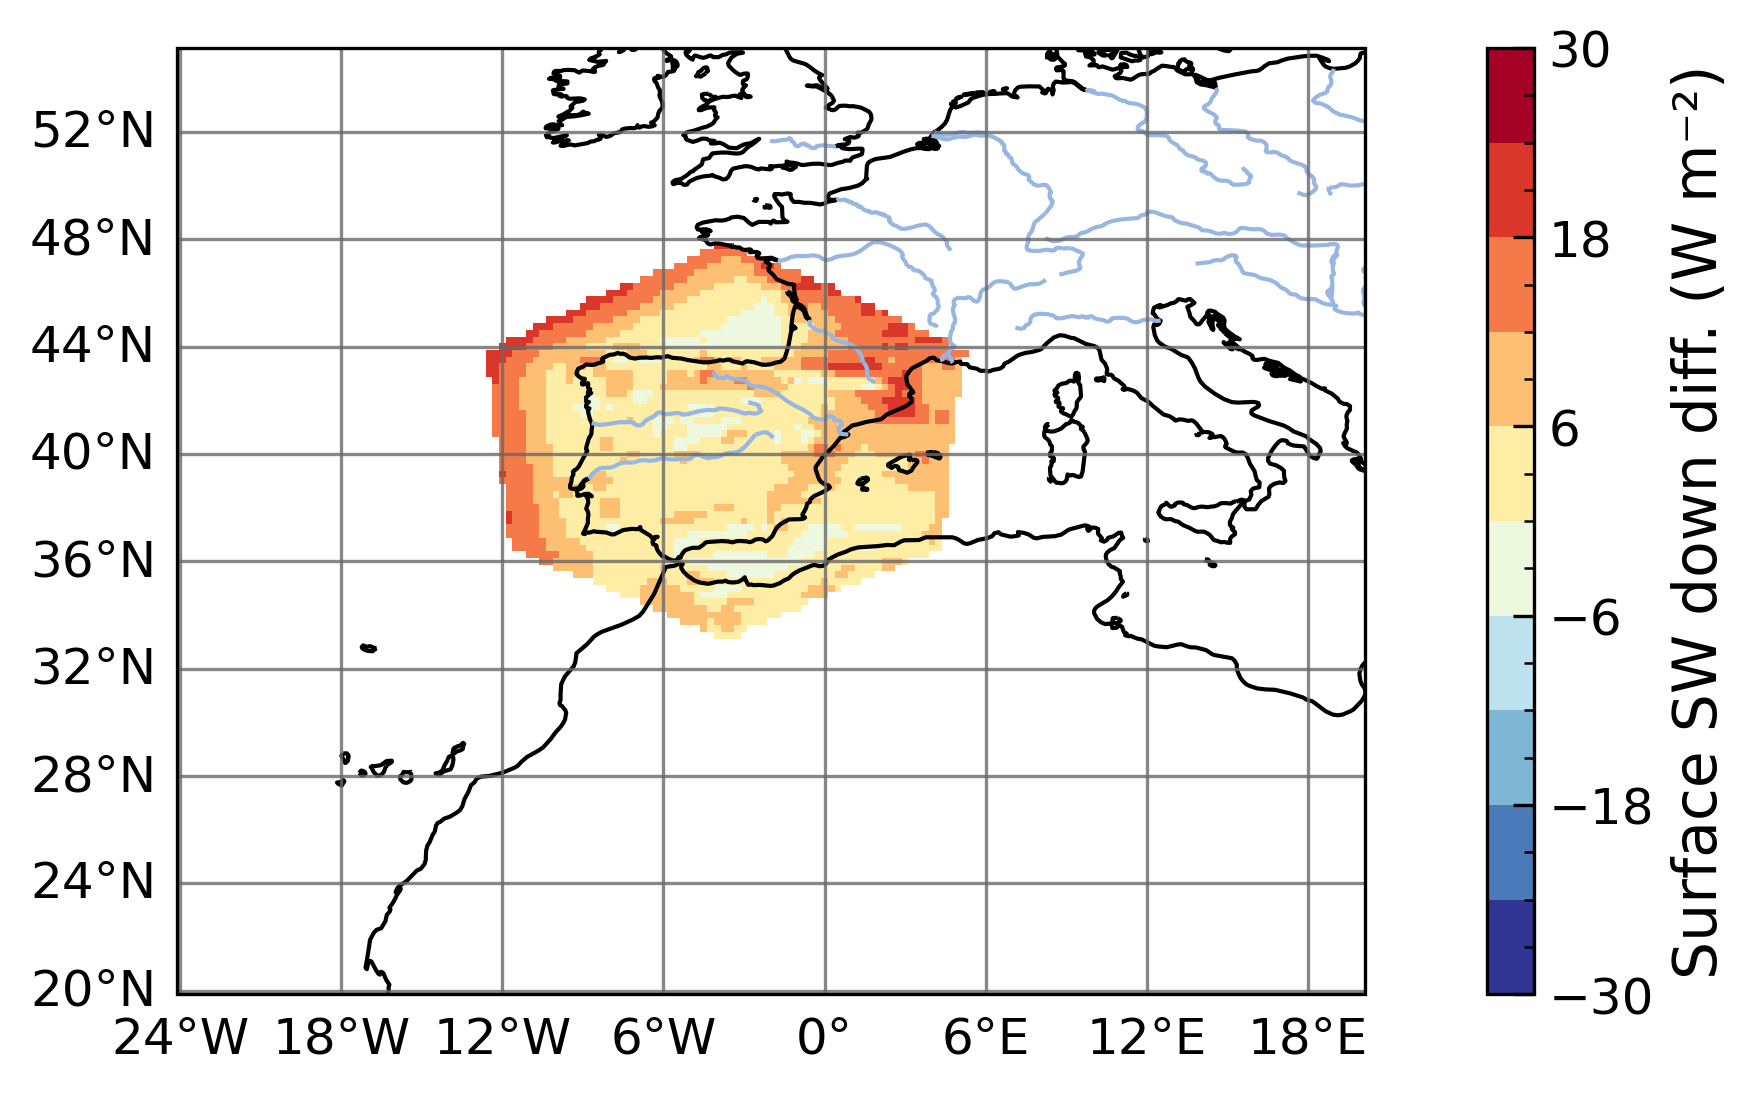
\includegraphics[width=\textwidth]{images/chap4/domain_size/diff_map_SWdnSFC_era_LAM_1000km_NBP40.png}
        \end{subfigure} &
        \begin{subfigure}[b]{0.33\textwidth}
            \caption{Downwelling SW flux bias\\(W \persqm, \interd)}
            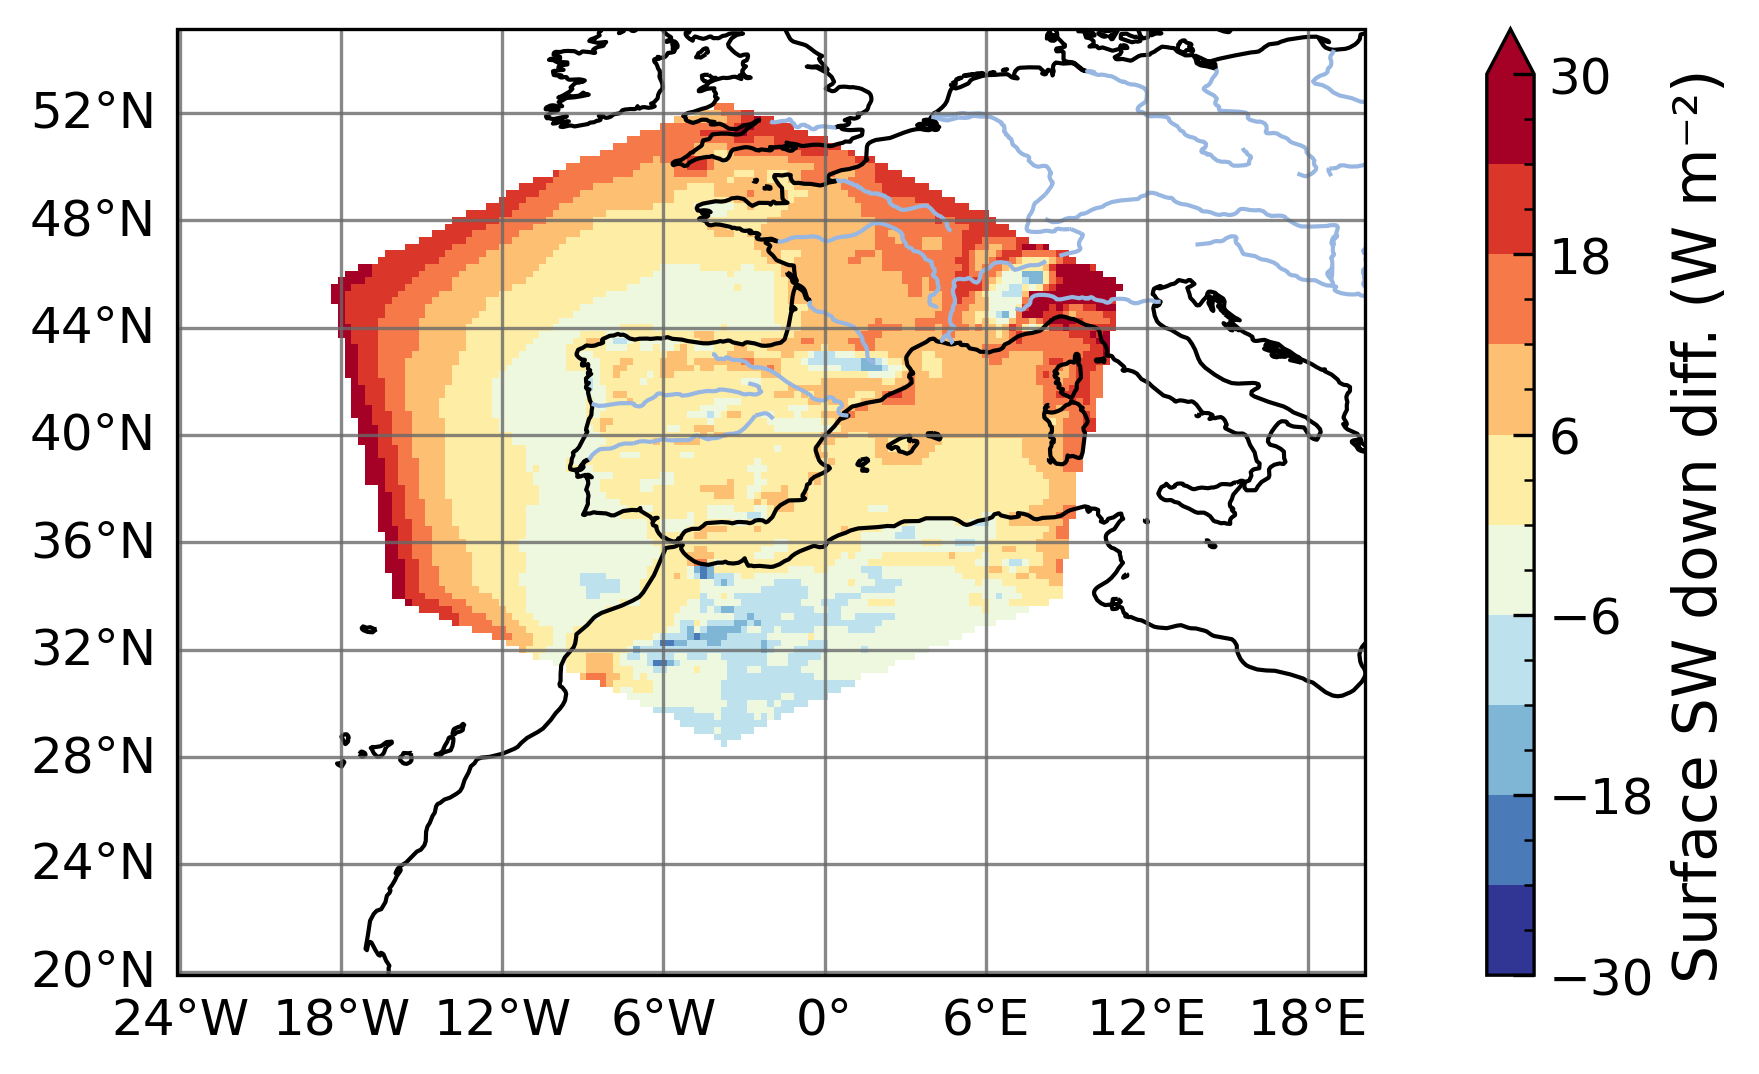
\includegraphics[width=\textwidth]{images/chap4/domain_size/diff_map_SWdnSFC_era_LAM_1500km_NBP60.png}
        \end{subfigure} &
        \begin{subfigure}[b]{0.33\textwidth}
            \caption{Downwelling SW flux bias\\(W \persqm, \larged)}
            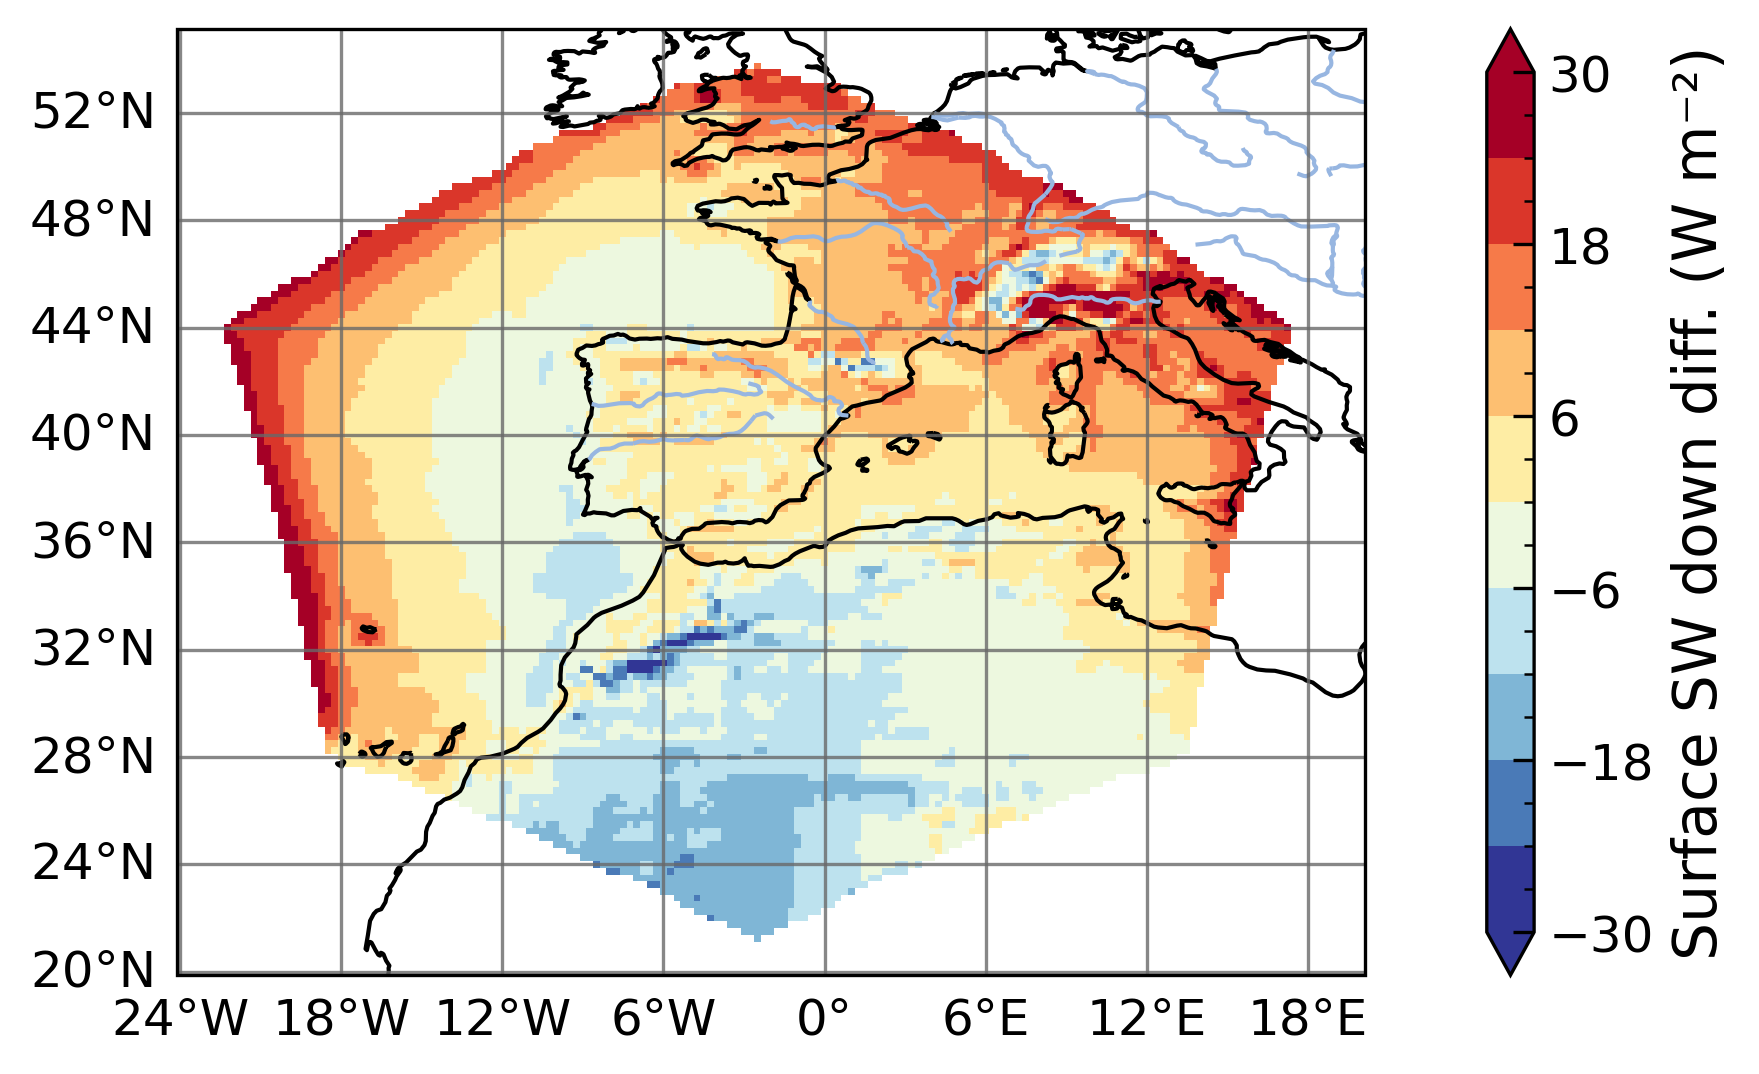
\includegraphics[width=\textwidth]{images/chap4/domain_size/diff_map_SWdnSFC_era_LAM_2000km_NBP80.png}
        \end{subfigure} \\
        
        %LWdn
        \begin{subfigure}[b]{0.33\textwidth}
            \caption{Downwelling LW flux bias\\(W \persqm, \smalld)}
            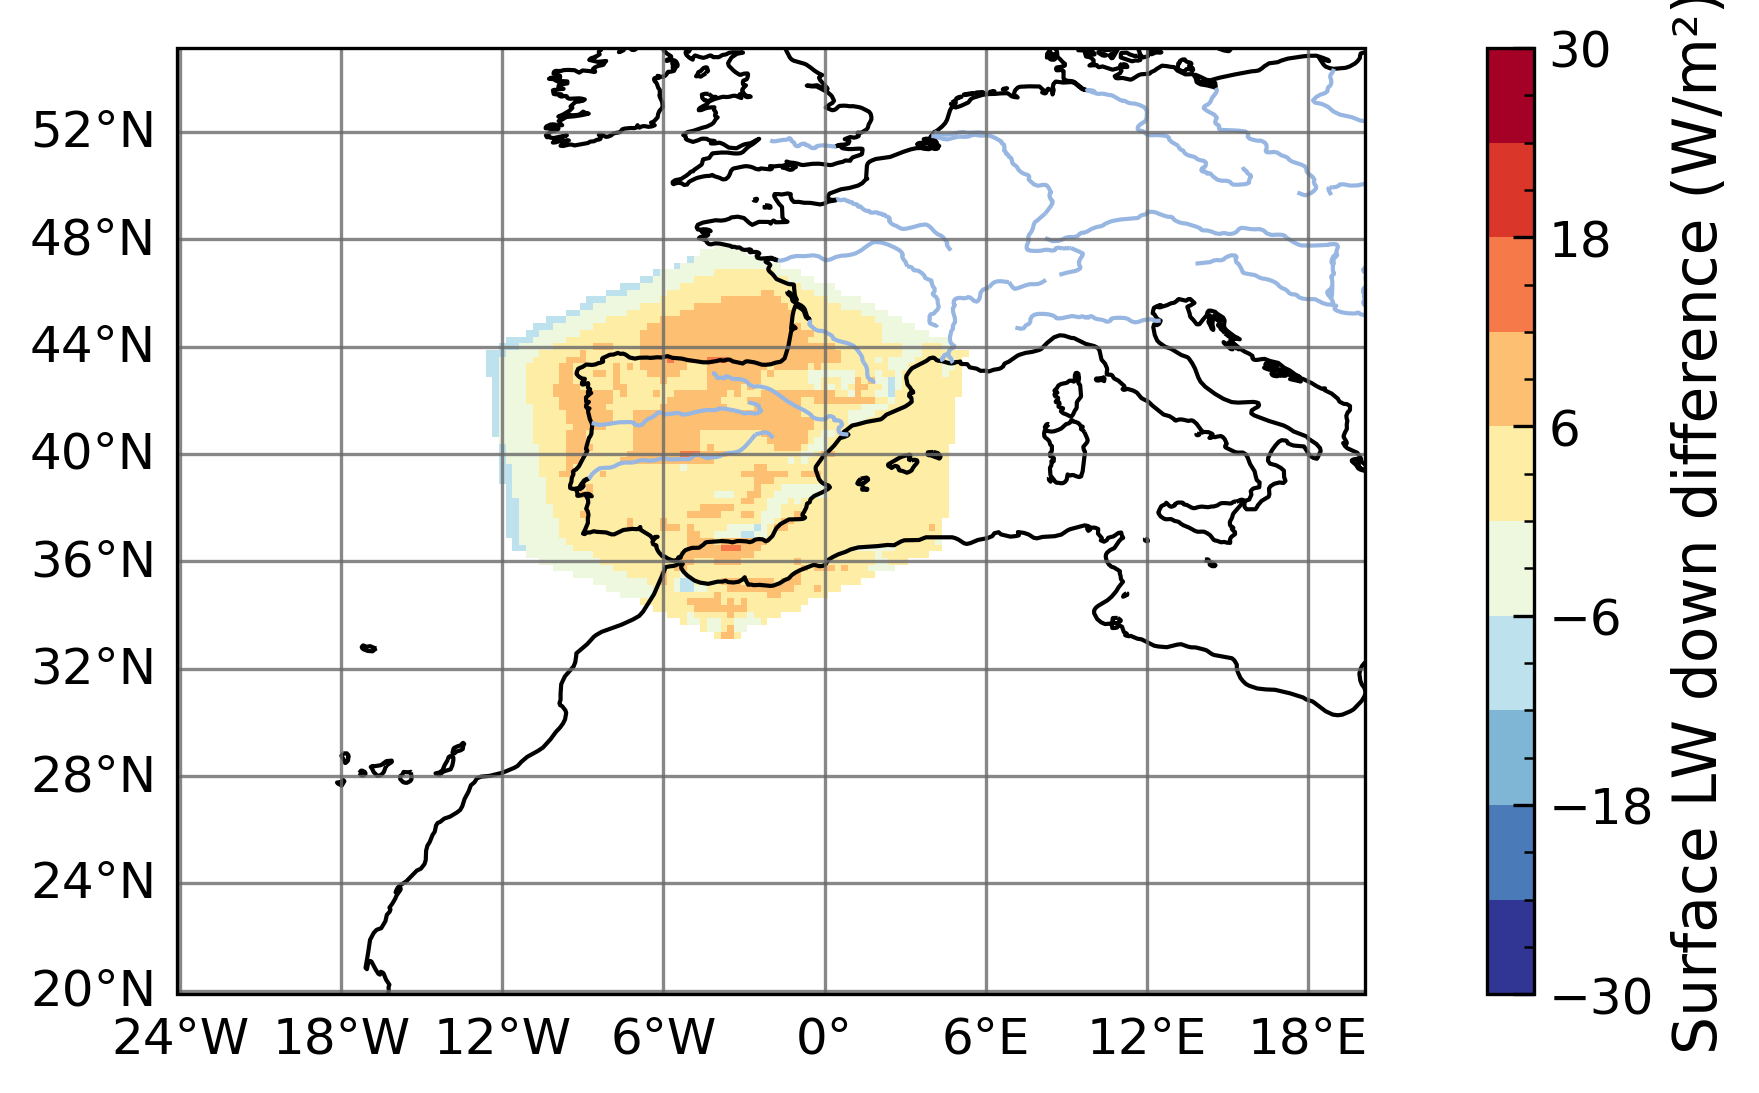
\includegraphics[width=\textwidth]{images/chap4/domain_size/diff_map_LWdnSFC_era_LAM_1000km_NBP40.png}
        \end{subfigure} &
        \begin{subfigure}[b]{0.33\textwidth}
            \caption{Downwelling LW flux bias\\(W \persqm, \interd)}
            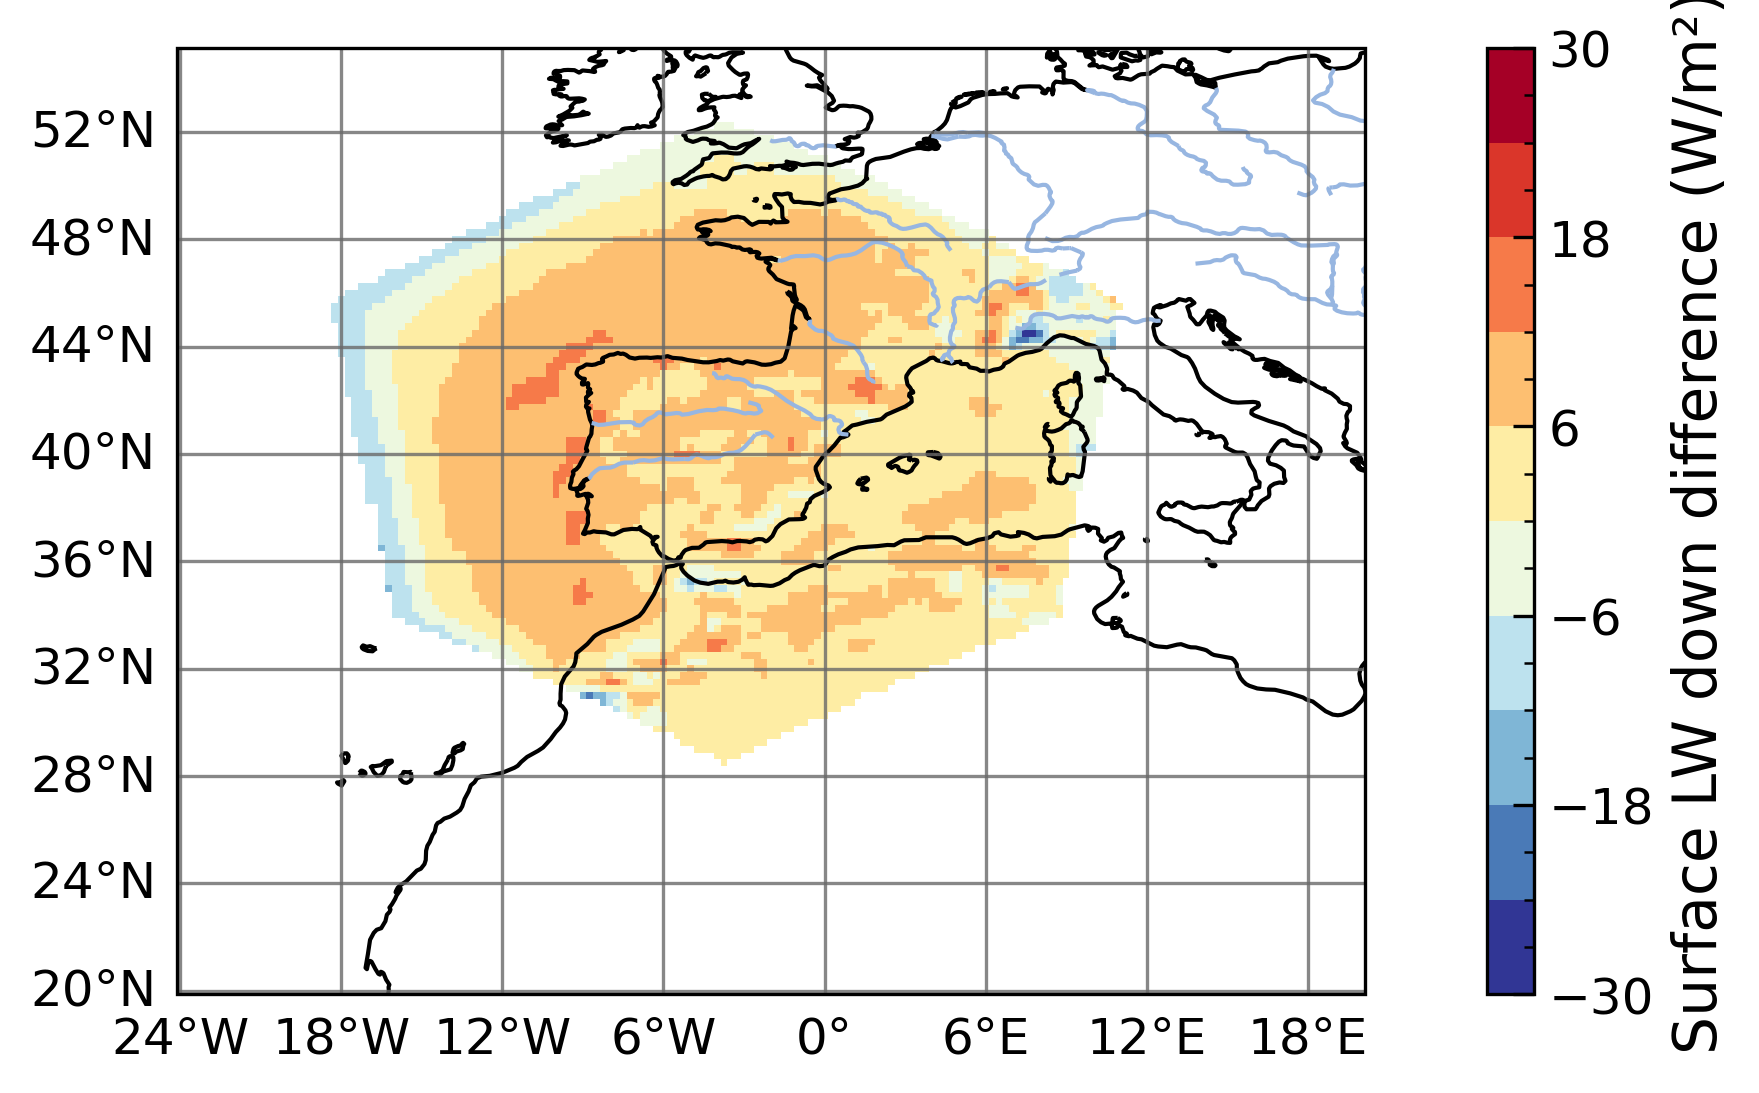
\includegraphics[width=\textwidth]{images/chap4/domain_size/diff_map_LWdnSFC_era_LAM_1500km_NBP60.png}
        \end{subfigure} &
        \begin{subfigure}[b]{0.33\textwidth}
            \caption{Downwelling LW flux bias\\(W \persqm, \larged)}
            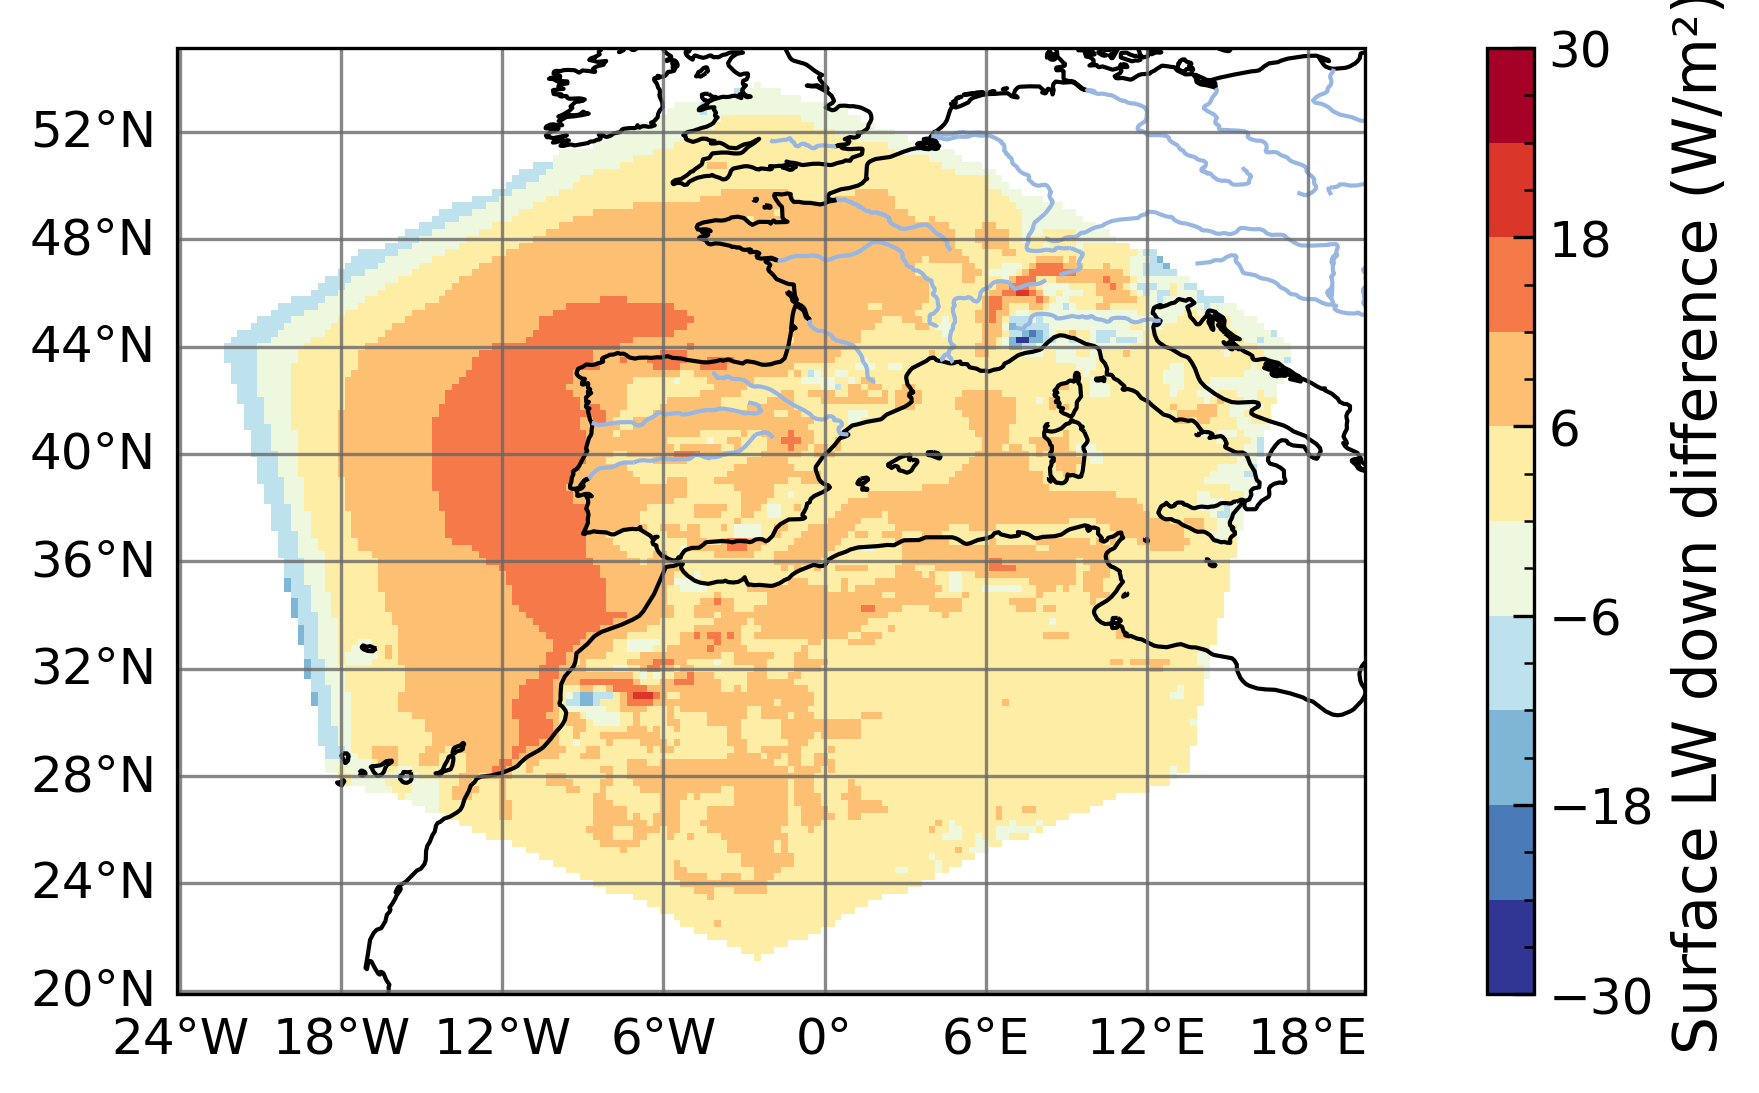
\includegraphics[width=\textwidth]{images/chap4/domain_size/diff_map_LWdnSFC_era_LAM_2000km_NBP80.png}
        \end{subfigure}
    \end{tabular}
    \caption{Cloud cover and downwelling radiative fluxes biases to ERA5 over 2010-2014 for three simulations with small, intermediate and large domain sizes.}
    \label{fig:domain_size_clouds_ERA_diff_maps}
\end{figure}

These results confirmed the hypothesis that the LAM is hindered from condensing water in the transition zone, where it is nudged towards the forcing data from the ERA5 reanalysis. This was attributed to the fact that the ERA5 data is obtained with a model that has its own physics scheme, possibly functioning very differently from the LMDZ physics, and that the continuous nudging does not give the physics of the LAM the freedom it needs to condense water. This explanation is very consistent with the very low values of cloud cover and precipitation in this zone.

In the free zone of the LAM, the model once again behaves normally, but can be influenced by the transition zone via the advection terms for atmospheric moisture computed by the dynamics. This means that the influence of the forcing and of the discrepancies between the physics of ERA5 and ICOLMDZ is not strictly confined to the transition zone.
The comparison of the three domain sizes show that in \smalld, the underestimation of precipitation is impacting some parts of the Peninsula, and that biases in ET are not limited to the edges but extended to large portions of the continental study area. With the two larger domains, although some biases persist over the Peninsula, their structure suggests that they are not the direct consequence of the discrepancies in the transition zone. Clear progress in the consistency of the LAM was therefore achieved by changing from the small to the intermediate domain. As there was no obvious improvements between the intermediate and large domain, the less computationally-intensive \interd simulation setup with $R_{domain} = 1500$ km and $NBP = 60$ was used for the rest of the study (results presented in Section \ref{sec:article1} and Chapter \ref{chap:liaise}).

Meanwhile, to explore the hypothesis that the biases in the transition zone are due to discrepancies between the physics of ICOLMDZ and ERA5, LAM simulations were run using a global ICOLMDZOR simulation as the source for the lateral boundary conditions. The results of this analysis are presented in the following Section \ref{sec:forcing_source}.

\clearpage

\section{Impact of the source of the lateral forcing}
\label{sec:forcing_source}

Here, two simulations using the small simulation domain over the period 2010-2022 are compared to assess the influence of the source used for the lateral forcing: one with forcing data from the ERA5 reanalysis (\forcingERA) and one using outputs of a global ICOLMDZOR simulation as forcing data (\forcingICO). 
The \forcingICO simulation was run by Frédérique Cheruy, and Mariame Maiga contributed to the analysis during her internship.

%figure : maps of diff vs ERA for 2 forcing sources
\begin{figure}[!h]
% \begin{figure}[b]
    \centering
    \begin{tabular}{cc}
        %precip
        \begin{subfigure}[b]{0.33\textwidth}
            \caption{Precipitation bias\\(mm \perday, \forcingERA)}
            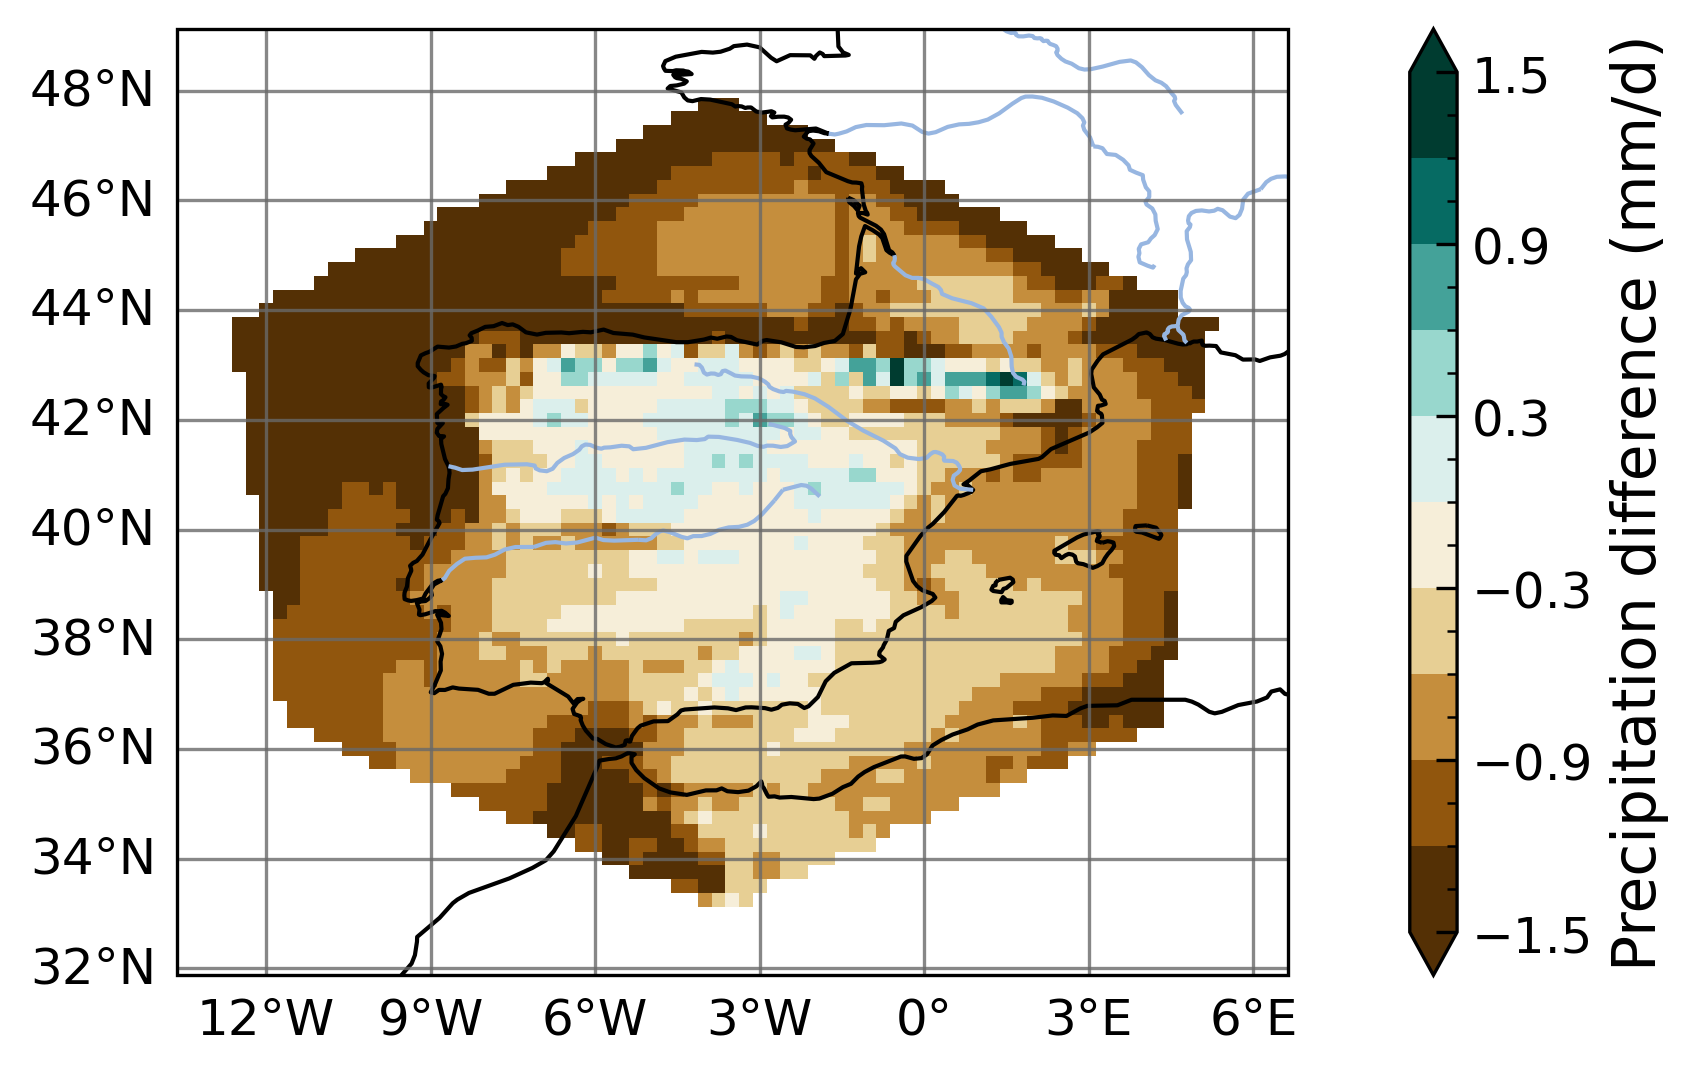
\includegraphics[width=\textwidth]{images/chap4/forcing_source/diff_map_precip_era_era.png}
        \end{subfigure} &
        \begin{subfigure}[b]{0.33\textwidth}
            \caption{Precipitation bias\\(mm \perday, \forcingICO)}
            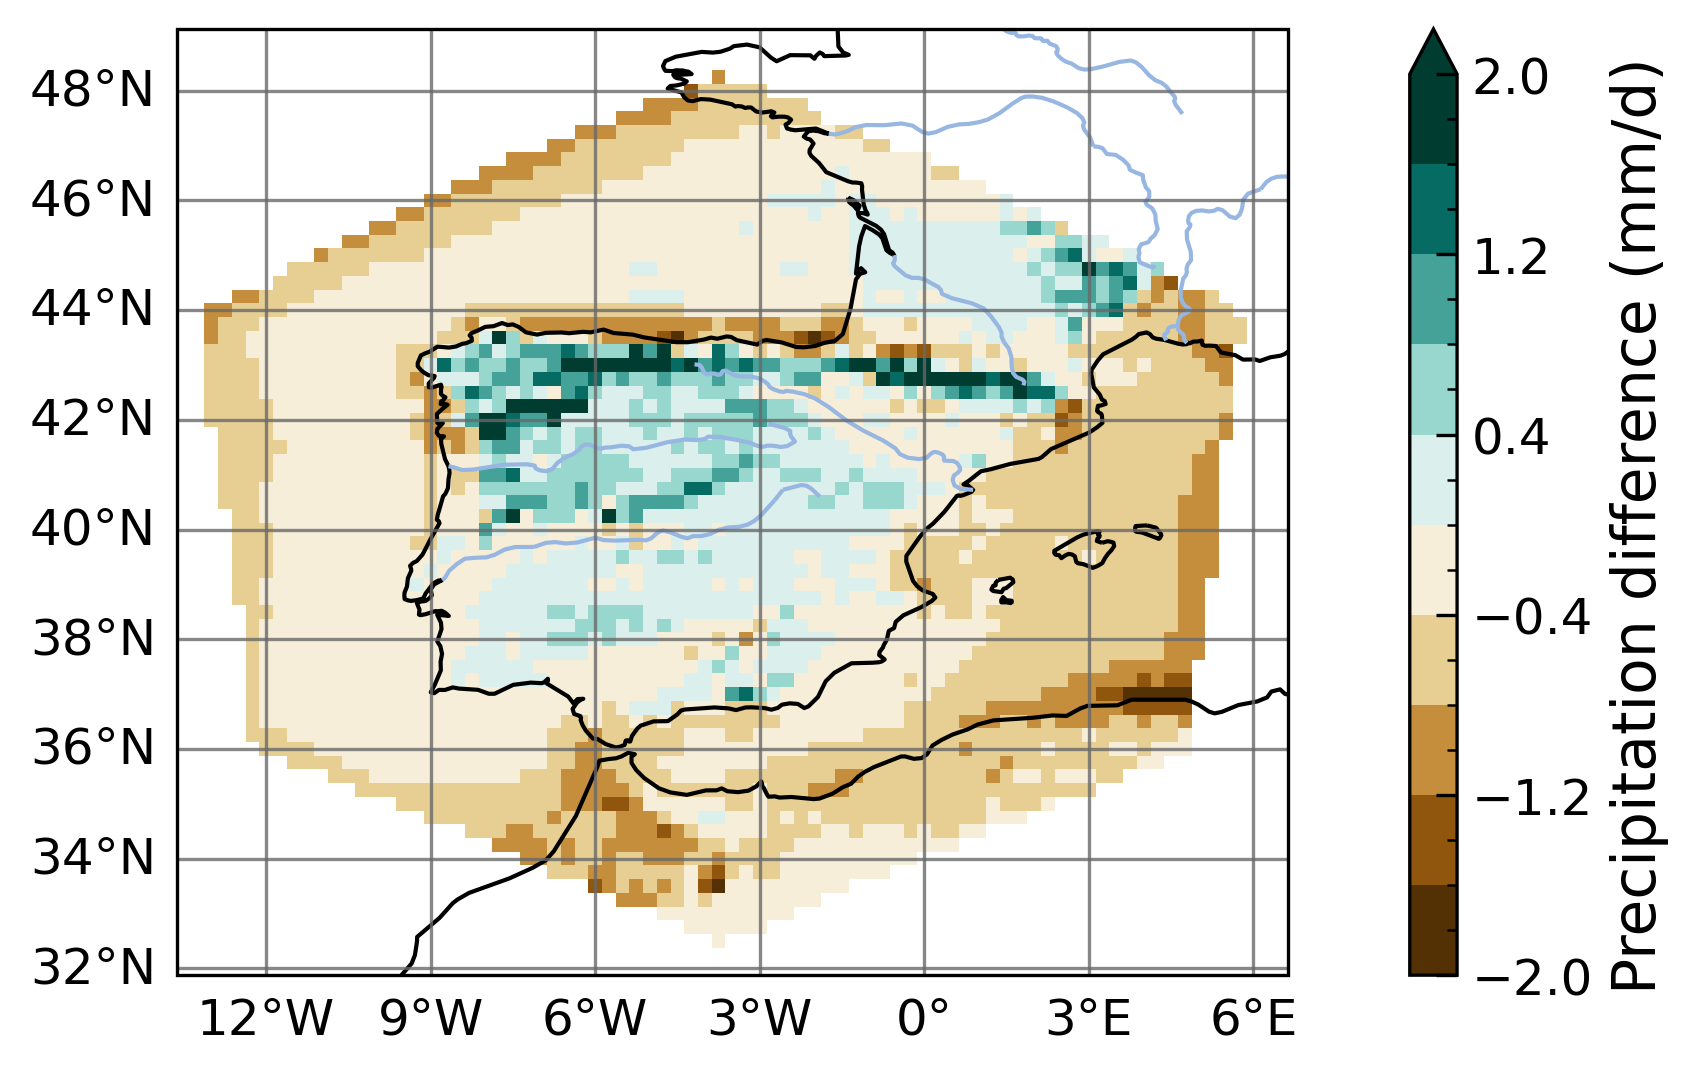
\includegraphics[width=\textwidth]{images/chap4/forcing_source/diff_map_precip_ico_era.png}
        \end{subfigure} \\
        %evap
        \begin{subfigure}[b]{0.33\textwidth}
            \caption{ET bias\\(mm \perday, \forcingERA)}
            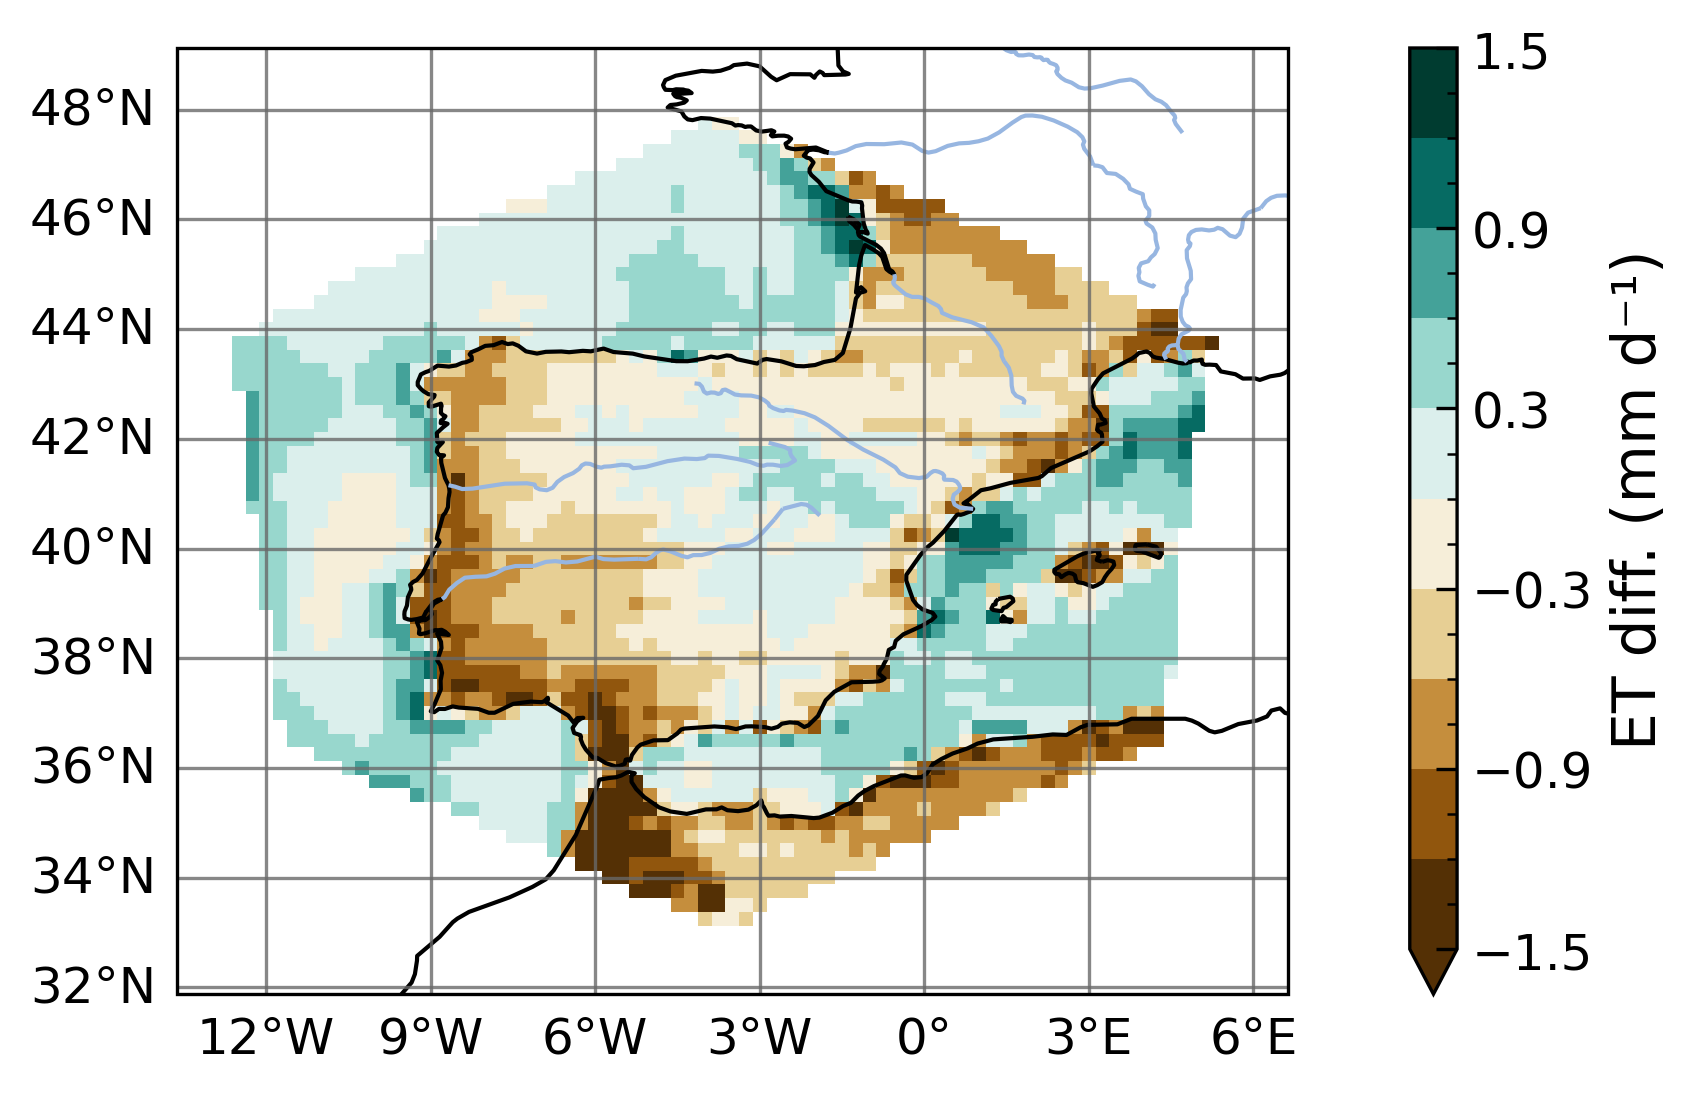
\includegraphics[width=\textwidth]{images/chap4/forcing_source/diff_map_evap_era_era.png}
        \end{subfigure} &
        \begin{subfigure}[b]{0.33\textwidth}
            \caption{ET bias\\(mm \perday, \forcingICO)}
            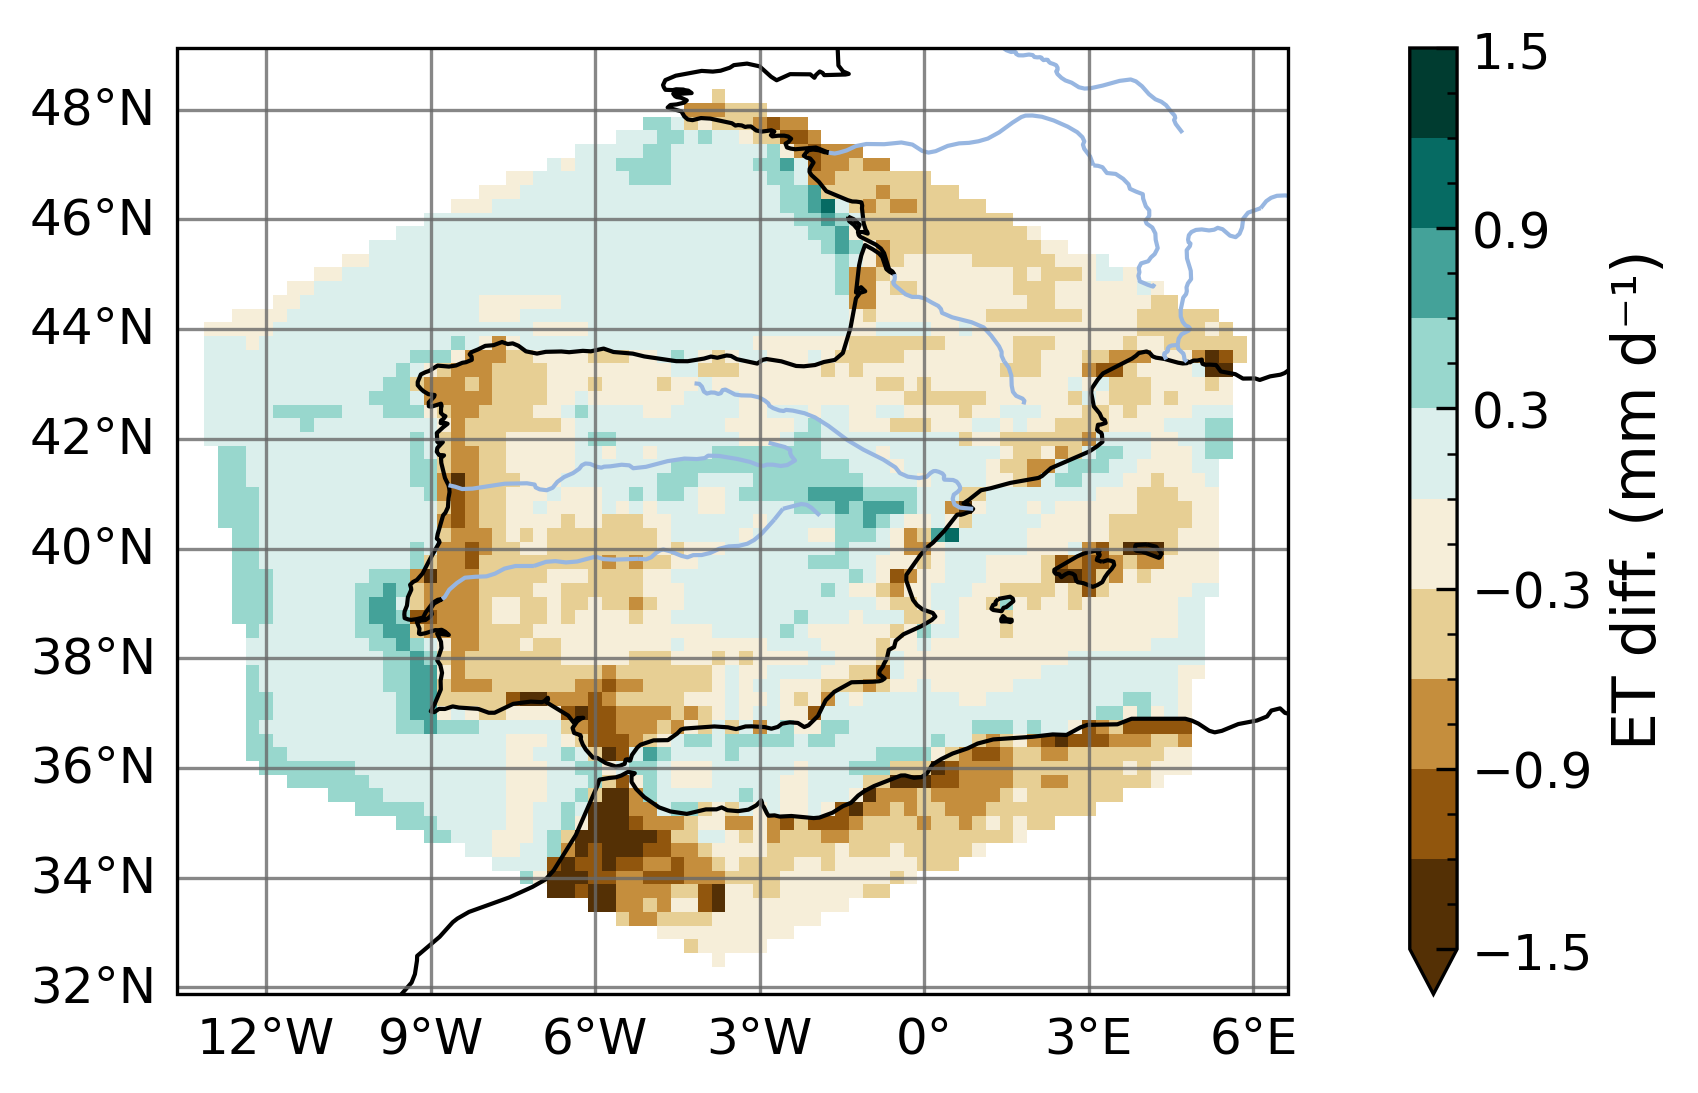
\includegraphics[width=\textwidth]{images/chap4/forcing_source/diff_map_evap_ico_era.png}
        \end{subfigure} \\
        %SWdn
        \begin{subfigure}[b]{0.33\textwidth}
            \caption{Downwelling SW flux bias\\(W \persqm, \forcingERA)}
            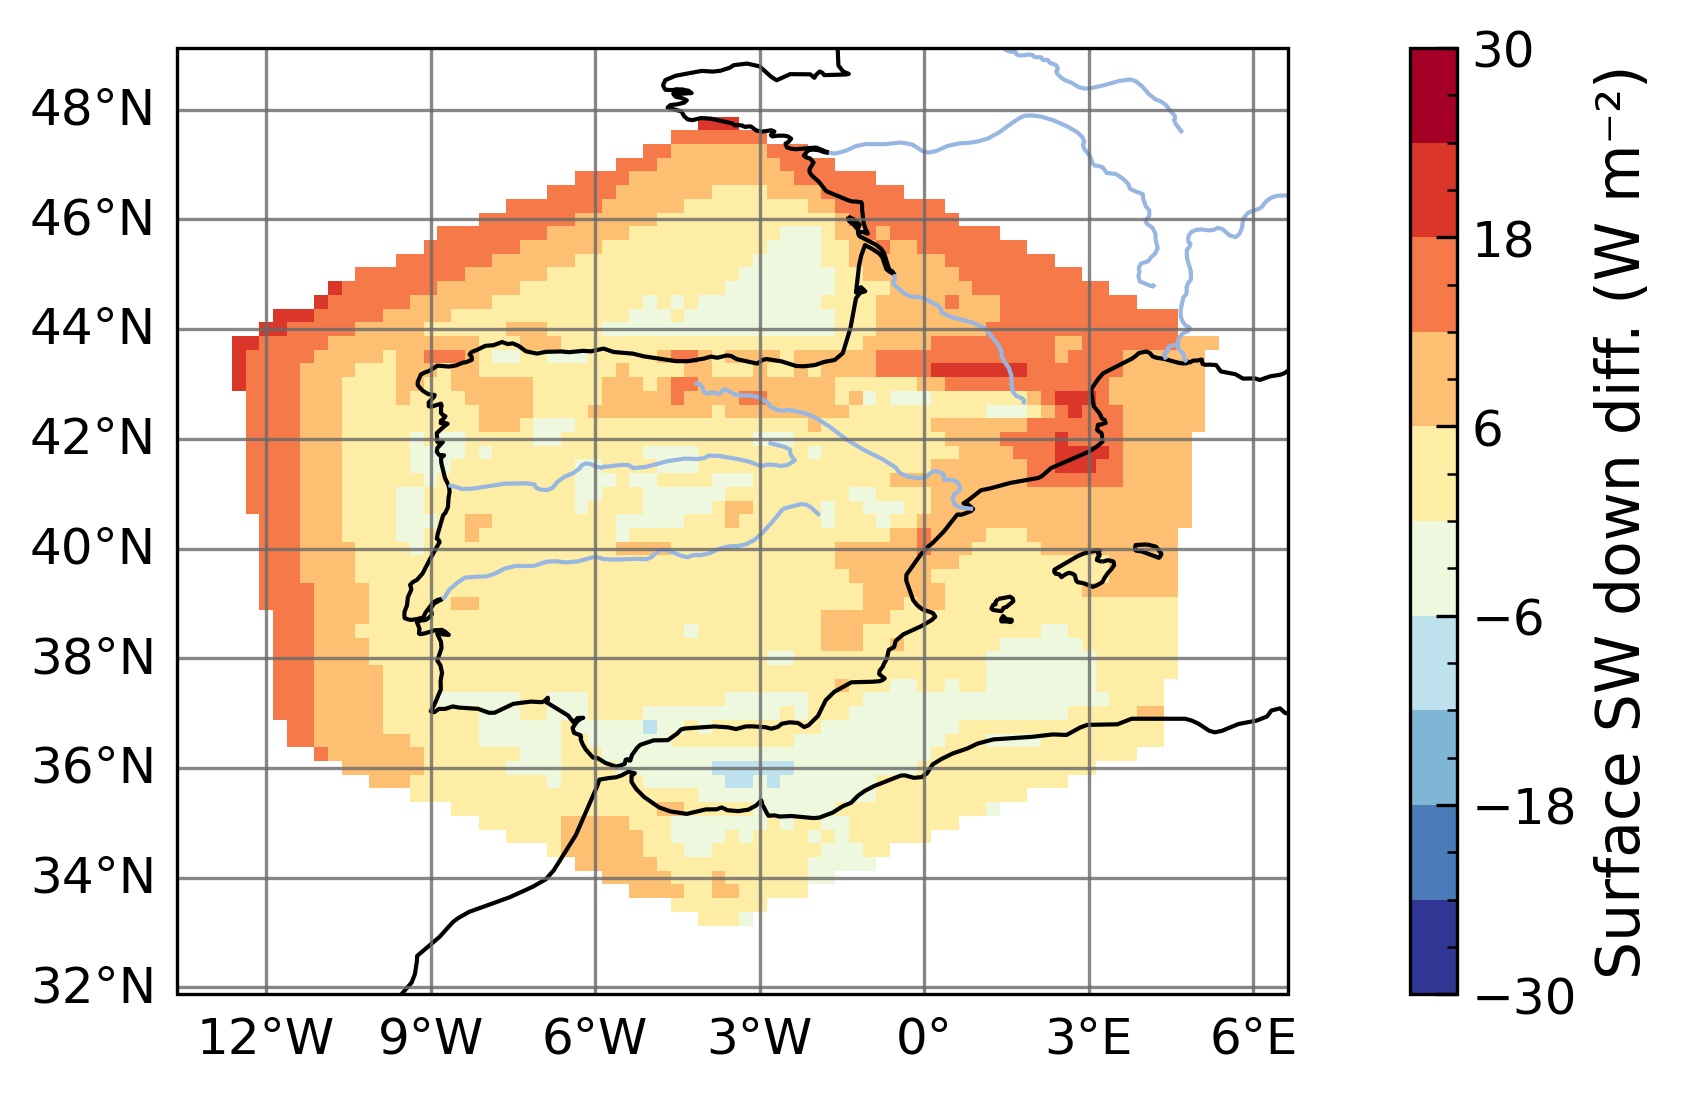
\includegraphics[width=\textwidth]{images/chap4/forcing_source/diff_map_SWdnSFC_era_era.png}
        \end{subfigure} &
        \begin{subfigure}[b]{0.33\textwidth}
            \caption{Downwelling SW flux bias\\(W \persqm, \forcingICO)}
            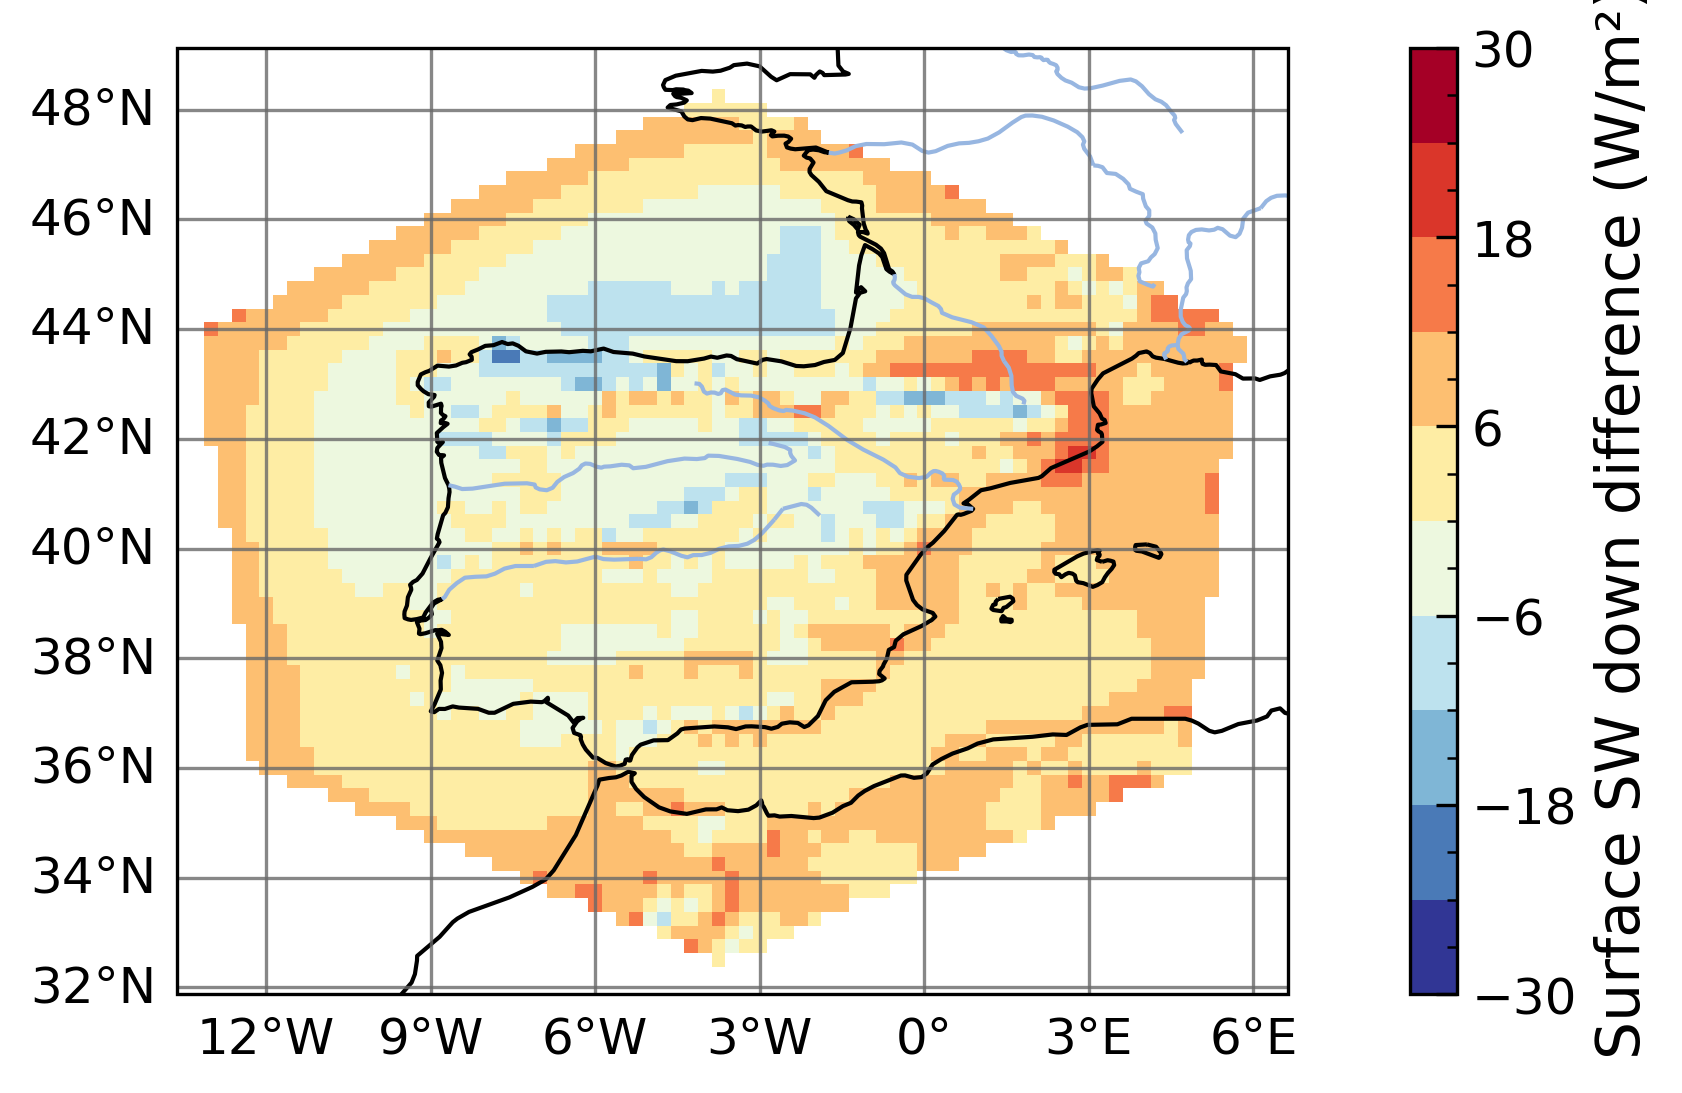
\includegraphics[width=\textwidth]{images/chap4/forcing_source/diff_map_SWdnSFC_ico_era.png}
        \end{subfigure}\\
        %LWdn
        \begin{subfigure}[b]{0.33\textwidth}
            \caption{Downwelling LW flux bias\\(W \persqm, \forcingERA)}
            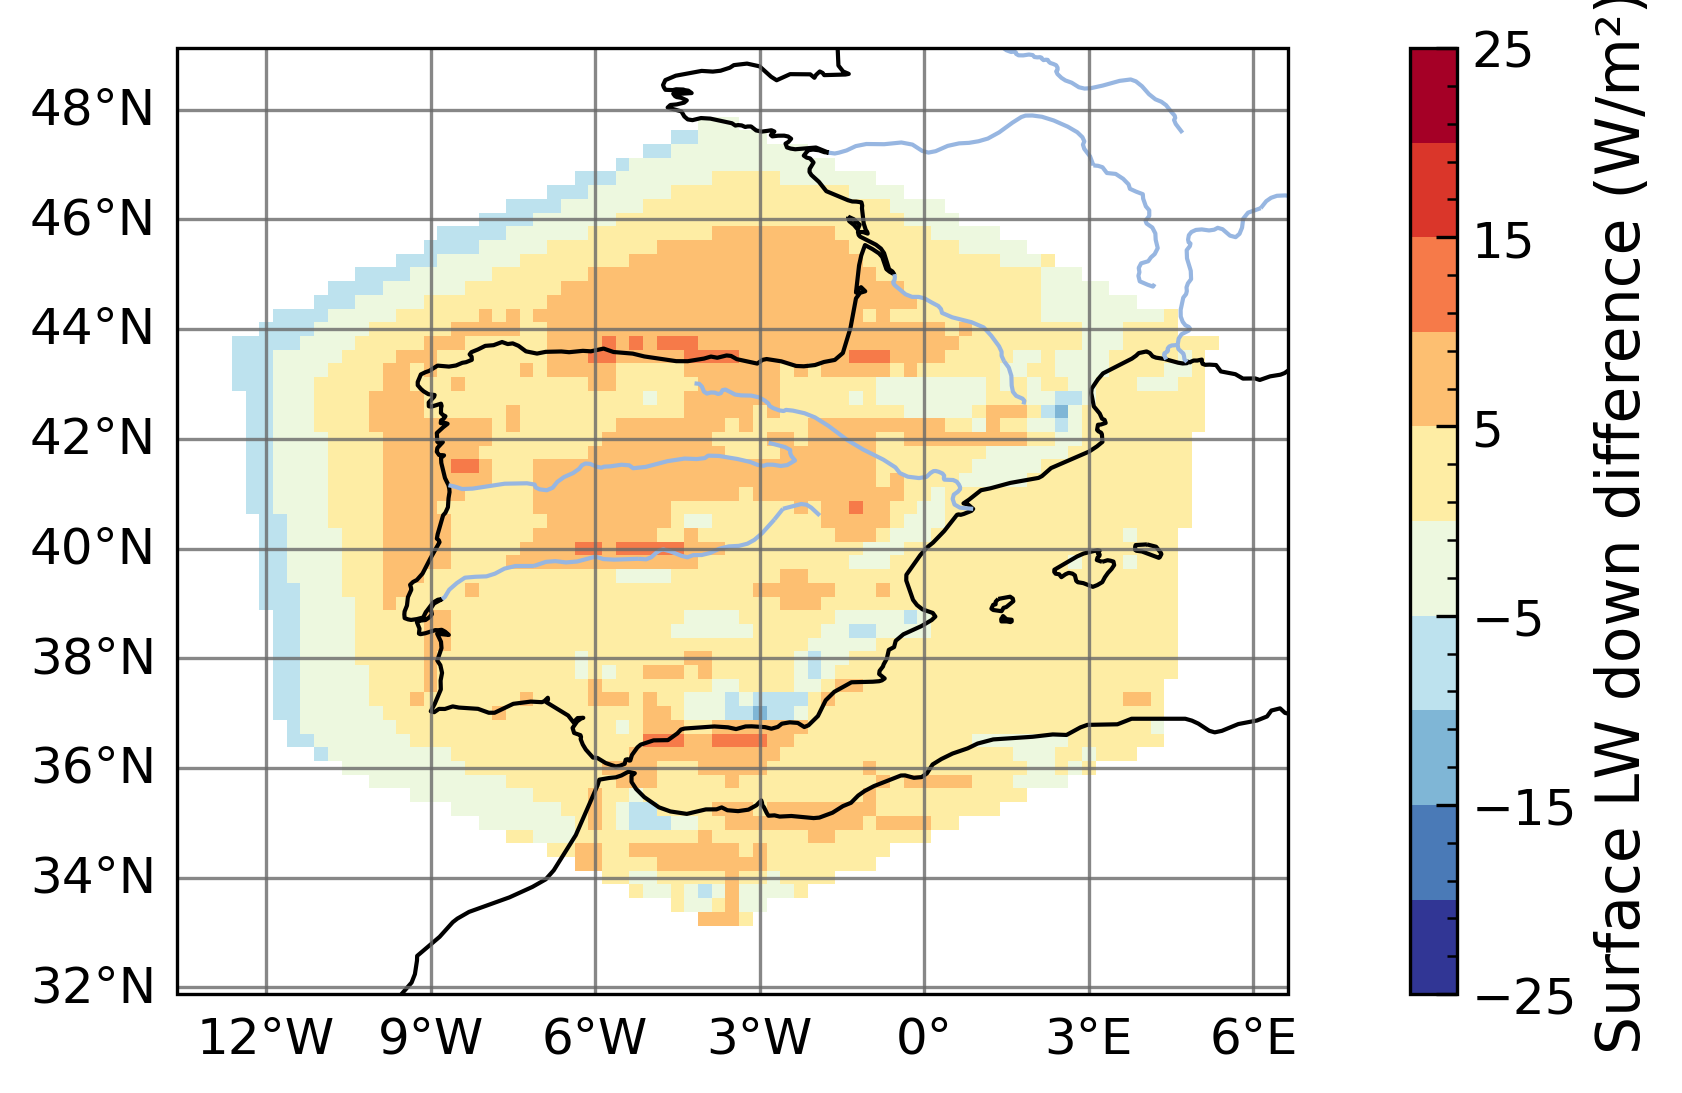
\includegraphics[width=\textwidth]{images/chap4/forcing_source/diff_map_LWdnSFC_era_era.png}
        \end{subfigure} &
        \begin{subfigure}[b]{0.33\textwidth}
            \caption{Downwelling LW flux bias\\(W \persqm, \forcingICO)}
            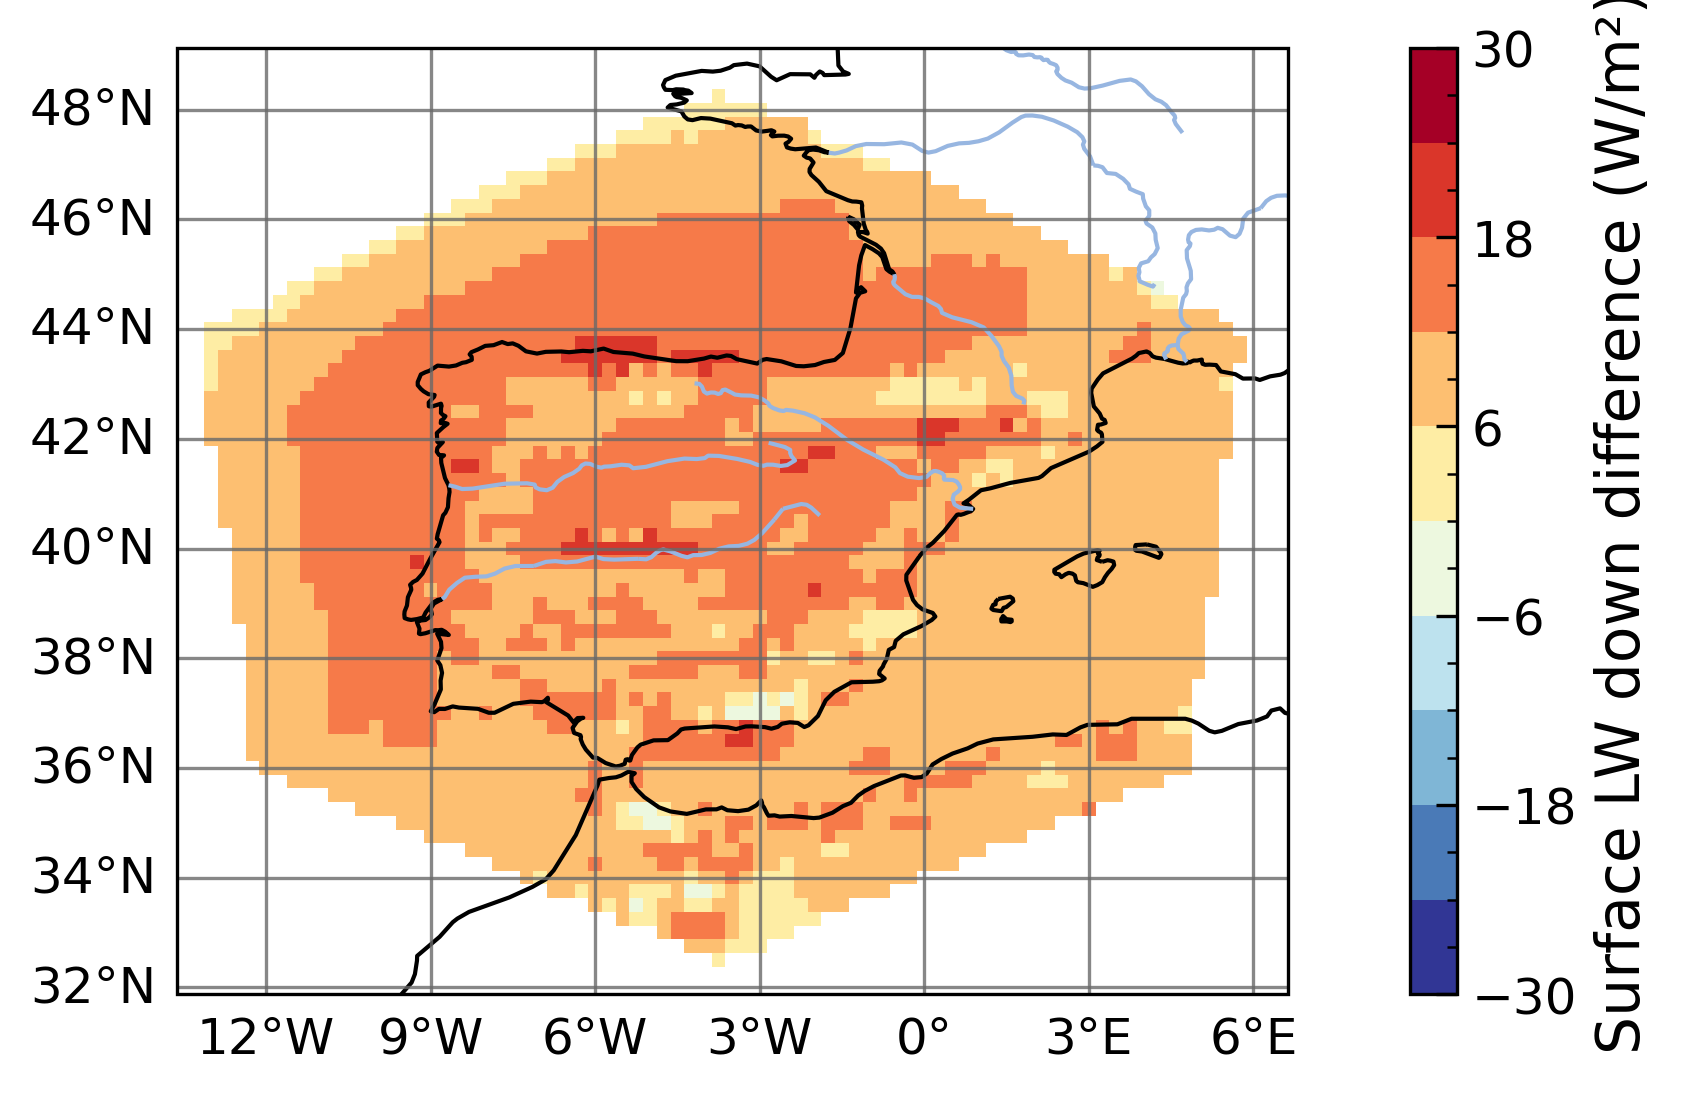
\includegraphics[width=\textwidth]{images/chap4/forcing_source/diff_map_LWdnSFC_ico_era.png}
        \end{subfigure}
    \end{tabular}
    \caption{Annual biases (2010-2022) of precipitation, evapotranspiration, and downwelling radiative fluxes for the simulations \forcingERA and \forcingICO, compared to ERA5.}
    \label{fig:forcing_source_ERA_diff_maps_endvars}
\end{figure}

In the transition zone, the biases in precipitation and downwelling shortwave flux compared to ERA5 are much smaller in \forcingICO than in \forcingERA, and more clearly limited to the edges of the domain (Fig. \ref{fig:forcing_source_ERA_diff_maps_endvars}a, b, e, f). For these variables, as well as for the downwelling longwave flux (Fig. \ref{fig:forcing_source_ERA_diff_maps_endvars}g, h), the spatial pattern of the bias in \forcingICO is similar to the patterns previously seen in simulations with the intermediate or large domain (Fig. \ref{fig:domain_size_P_ET_ERA_diff_maps} \ref{fig:domain_size_clouds_ERA_diff_maps}), confirming the idea that the model is much more consistent when it is forced by ICOLMDZOR. There is no clear improvement of ET over the Atlantic ocean, but over the Mediterranean, the underestimation is reversed to a small overestimation, as previously seen in simulations with larger domains (Fig. \ref{fig:domain_size_P_ET_ERA_diff_maps}e, f).
All these findings confirm that the behaviour of the LAM is dependent on the source of the lateral boundary conditions. Forcing it with outputs from a global ICOLMDZOR simulation rather than ERA5 allows a more consistent behaviour of the condensation scheme in the transition zone, and avoids the spread of the biases from the edges of the domain to the central free zone.

\hfill

However, the global ICOLMDZOR simulation is not a reanalysis and is not expected to reproduced observed synoptic conditions like ERA5. Since the period analysed here remains short compared to climatic time scales (13 years), inter-annual variability can lead to large differences between reality and the simulation. Therefore, the comparison of the \forcingICO to observed conditions reveals new biases. Over the Iberian Peninsula, precipitation is clearly overestimated in northern mountainous areas (Fig. \ref{fig:forcing_source_ERA_diff_maps_endvars}b), while the larger low cloud cover affects downwelling radiative fluxes along the Atlantic coast, leading to an underestimation of the shortwave flux and an overestimation of the longwave flux (Fig. \ref{fig:forcing_source_ERA_diff_maps_endvars}f, h) which were not present in \forcingERA.
To analyse this further, precipitation and ET in the two simulation were respectively compared to the GPCC and GLEAM products over the Iberian Peninsula, from 2010 to 2019 (Fig. \ref{fig:forcing_source_SC}).

%figure : SC of precip and evap with GLEAM and GPCC
\begin{figure}[htbp]
    \centering
    %precip
    \begin{subfigure}[b]{0.49\textwidth}
        \caption{Seasonal cycle of precipitation (2010-2019)}
        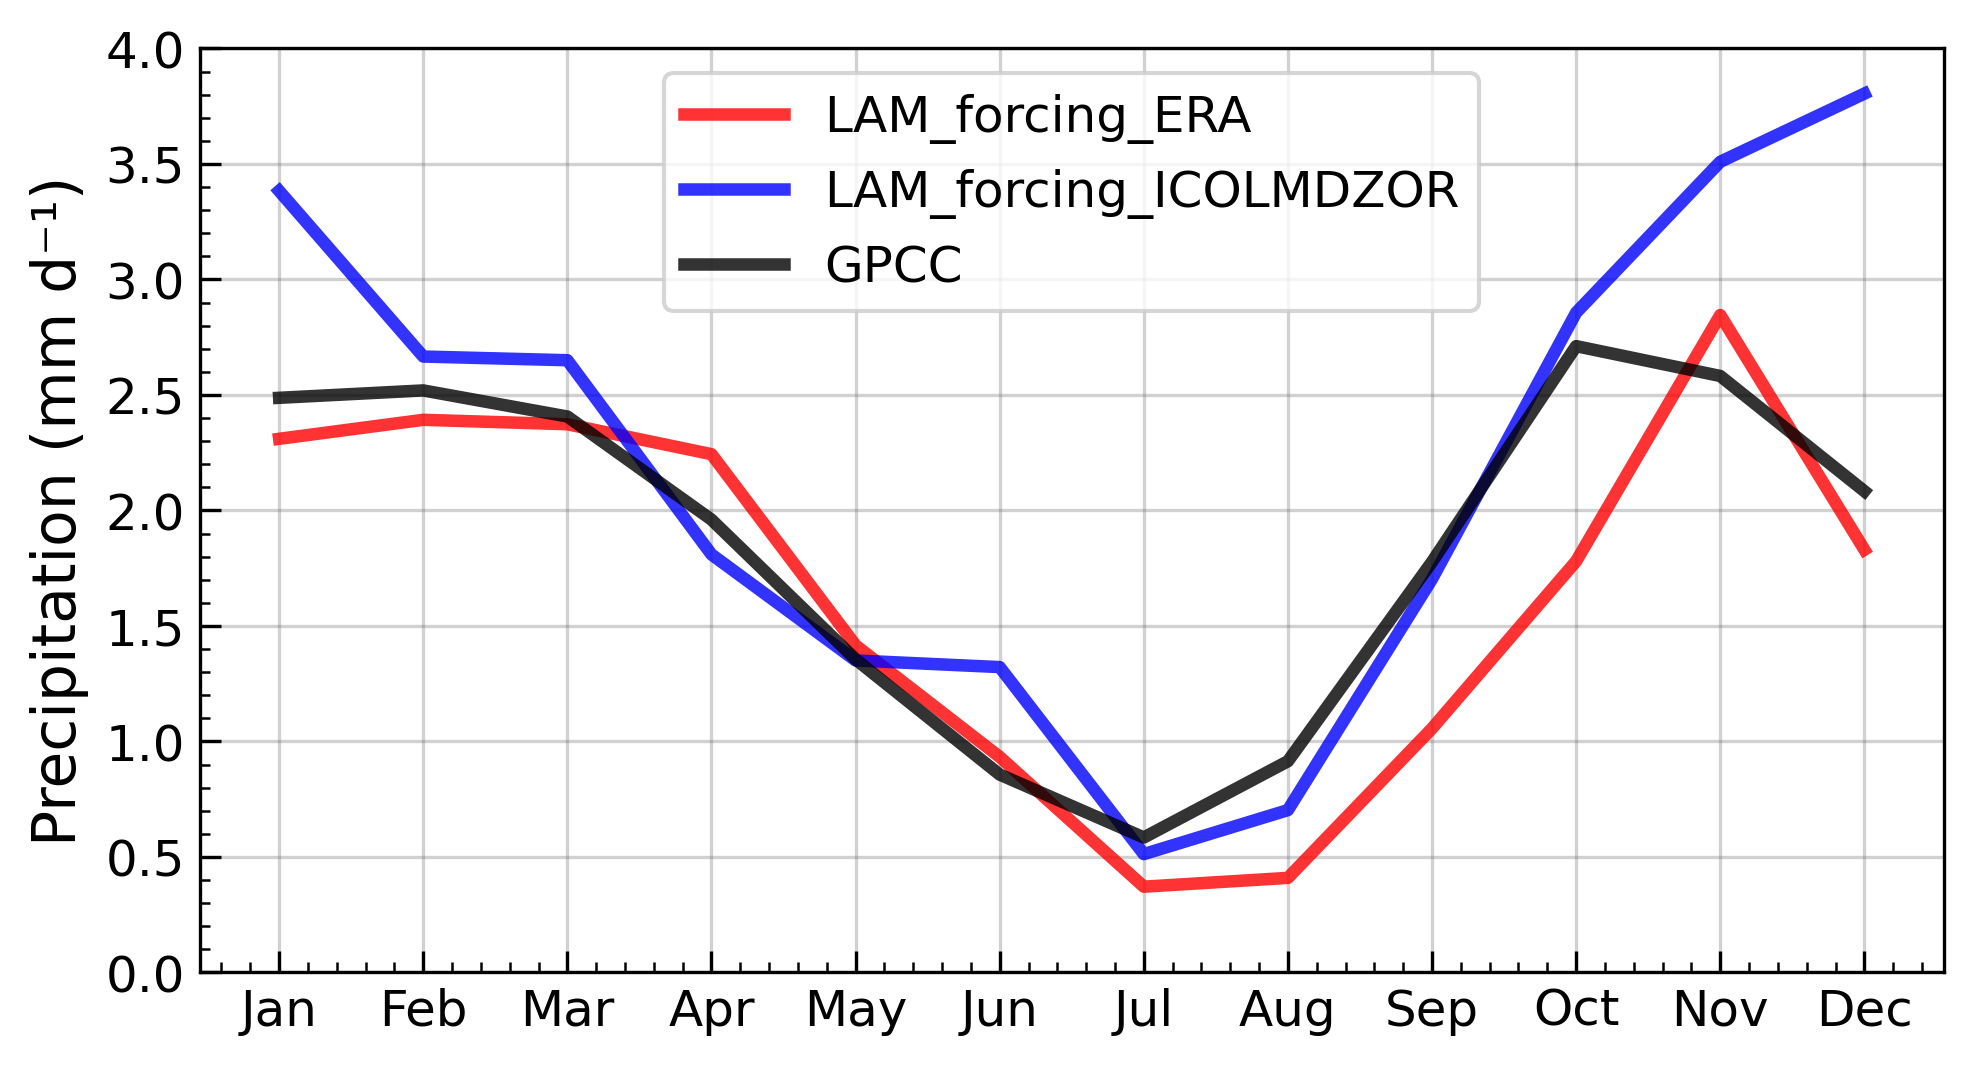
\includegraphics[width=\textwidth]{images/chap4/forcing_source/IP_seasonal_cycle_precip.png}
    \end{subfigure}
    \begin{subfigure}[b]{0.49\textwidth}
        \caption{Seasonal cycle of ET (2010-2019)}
        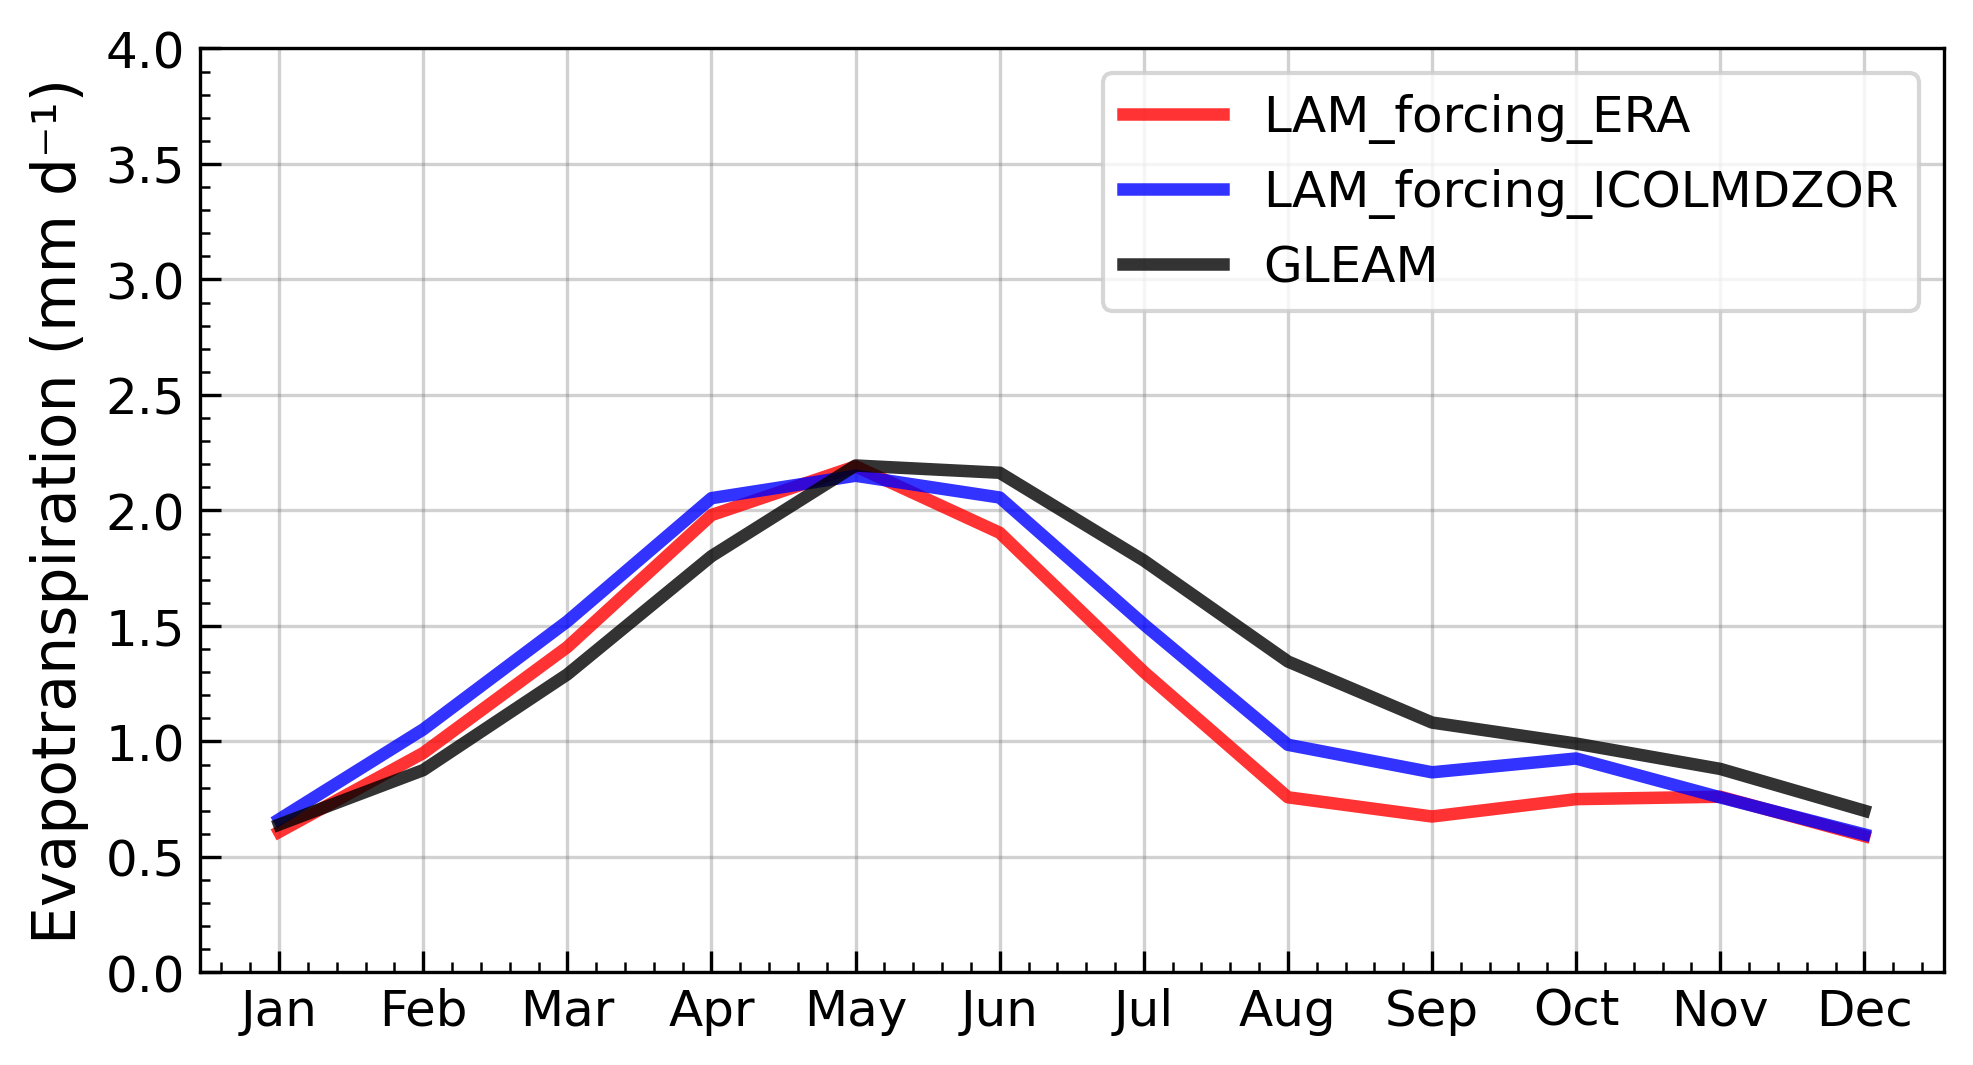
\includegraphics[width=\textwidth]{images/chap4/forcing_source/IP_seasonal_cycle_evap.png}
    \end{subfigure}
    \caption{Mean seasonal cycle of precipitation and evapotranspiration, on average over the Iberian Peninsula, for the LAM forced by ERA (red) and forced by ICOLMDZOR (blue), and the GPCC and GLEAM products (2010-2019).}
    \label{fig:forcing_source_SC}
\end{figure}

When forced with ICOLMDZOR rather than ERA5, the LAM simulates similar amounts of precipitation in spring and larger precipitation from July to October (Fig. \ref{fig:forcing_source_SC}a) matching GPCC. This improvement is possible because the precipitation underestimation in the transition zone is largely reduced in \forcingICO compared to \forcingERA, and does not affect the central part of the domain. 
However, in winter, the LAM now strongly overestimates precipitation, mainly due to excessive snow and rainfall in mountainous areas, as visible in Fig. \ref{fig:forcing_source_ERA_diff_maps_endvars}b. This is a known bias of climate models and was already described for the LMDZ physics in particular \citep{arjdal_modeling_2024, adhikari_evaluation_2024}. 
Over this season, model performance may not be improved by changing the forcing source, but it has the advantage of being self-consistent over the domain, and of producing biases that have already been studied and analysed in the IPSL modelling community.

The increase in summer precipitation in \forcingICO lead to an increase in ET over the Peninsula (Fig. \ref{fig:forcing_source_SC}b), although a gap remains between the GLEAM product and the model. This dry biasmight derive from various causes, among which an underestimation of the downwelling shortwave radiation in some regions, the parametrization of evapotranspiration components in the LSM, and the absence of irrigation in the simulations. In other seasons, the difference between the two simulation remains limited. In particular, the increases in precipitation in winter do not lead to significant changes in ET since in the mountainous areas where they occur, precipitation is already large and ET is not limited by the available soil moisture.

\hfill

In summary, the comparison of the two LAM simulations, \forcingERA and \forcingICO, corroborated the hypothesis that the inconsistent behaviour of the LAM in the transition zone was due to discrepancies between the physics used to produce the ERA5 reanalysis and the LMDZ physics of the LAM. Indeed, biases on the edges of the domain are largely reduced when ICOLMDZOR outputs are used as forcing data, and their influence on the Iberian Peninsula almost disappears. However, although the LAM gains consistency, its performance compared to observation-based reference products may not be systematically improved, because the ICOLMDZOR model has its own biases, that can be present in the forcing and perpetuated by the LAM, as seen with the overestimation of precipitation over mountainous areas in winter.

\clearpage

\section{Impact of the forcing file sampling frequency}
\label{sec:forcing_frequency}
%figure : maps of diff vs ERA for 2 forcing sampling freqs
\begin{figure}[!h]
    \centering
    \begin{tabular}{cc}
        %precip
        \begin{subfigure}[b]{0.33\textwidth}
            \caption{Precipitation bias\\(mm \perday, \forcingoneh)}
            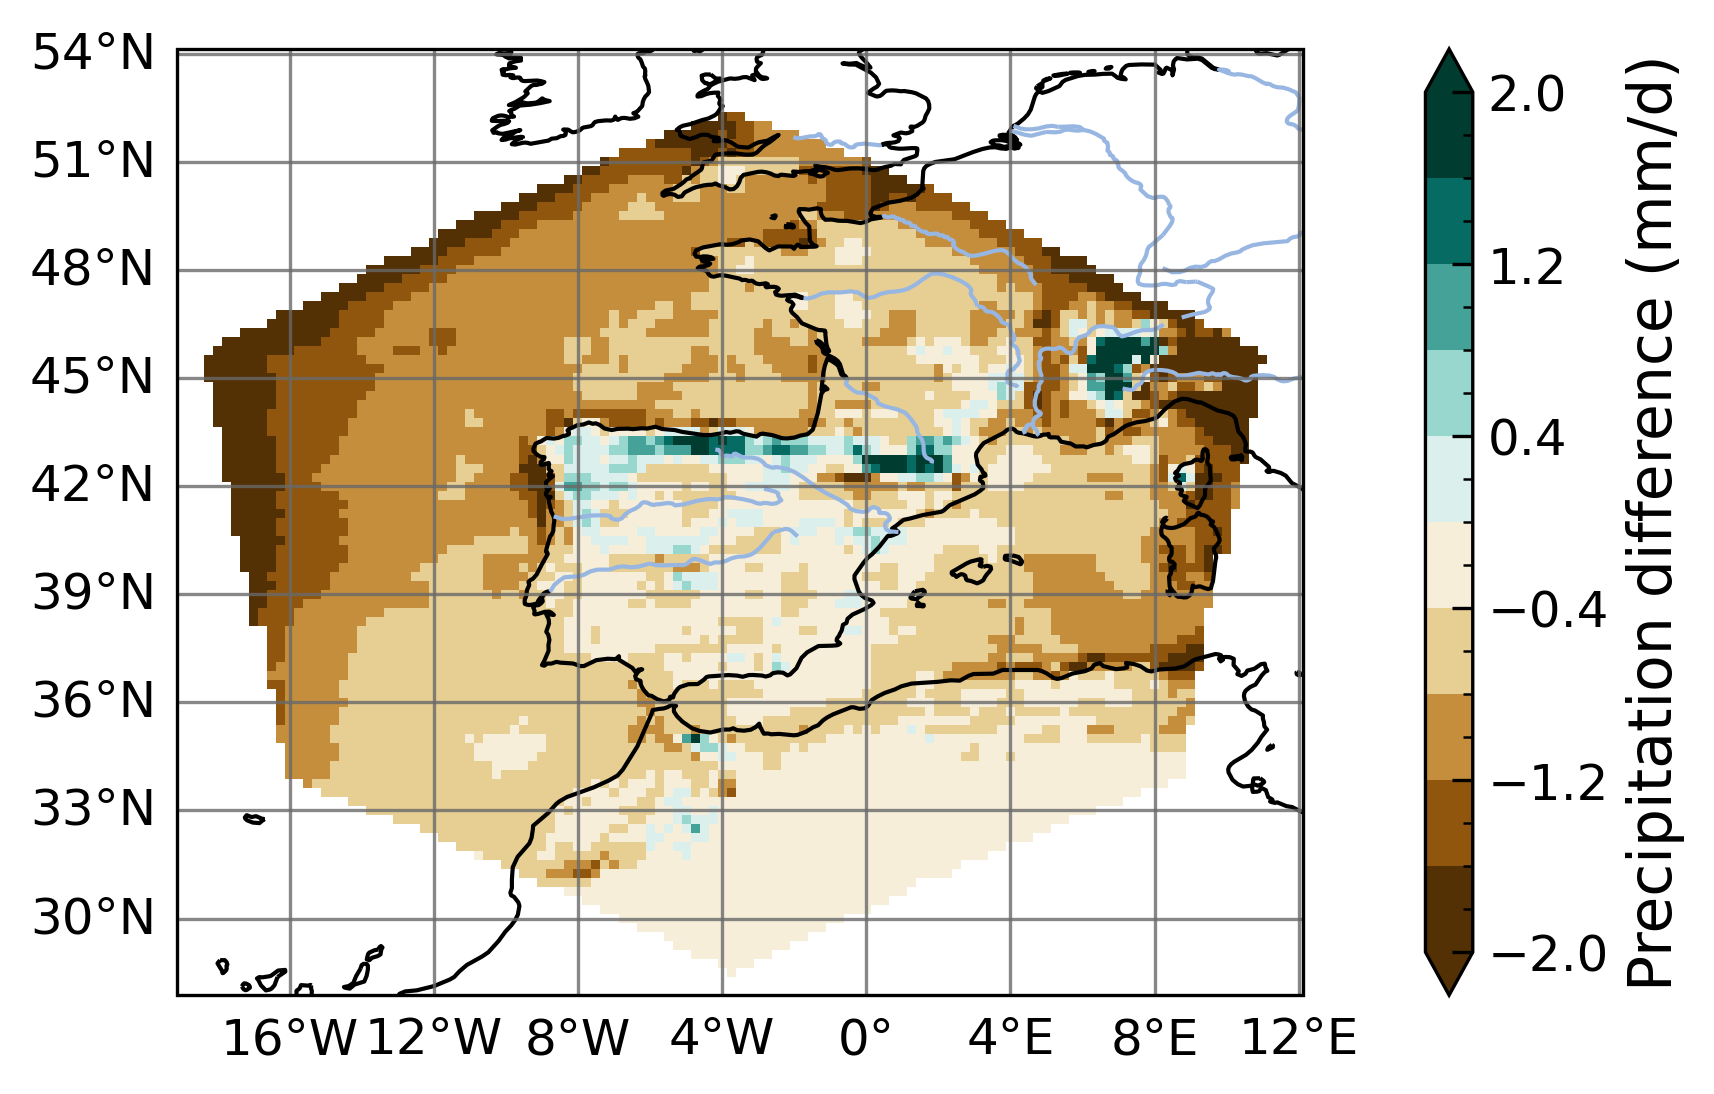
\includegraphics[width=\textwidth]{images/chap4/forcing_sampling_freq/diff_map_precip_lmdz1h_era.png}
        \end{subfigure} &
        \begin{subfigure}[b]{0.33\textwidth}
            \caption{Precipitation bias\\(mm \perday, \forcingsixh)}
            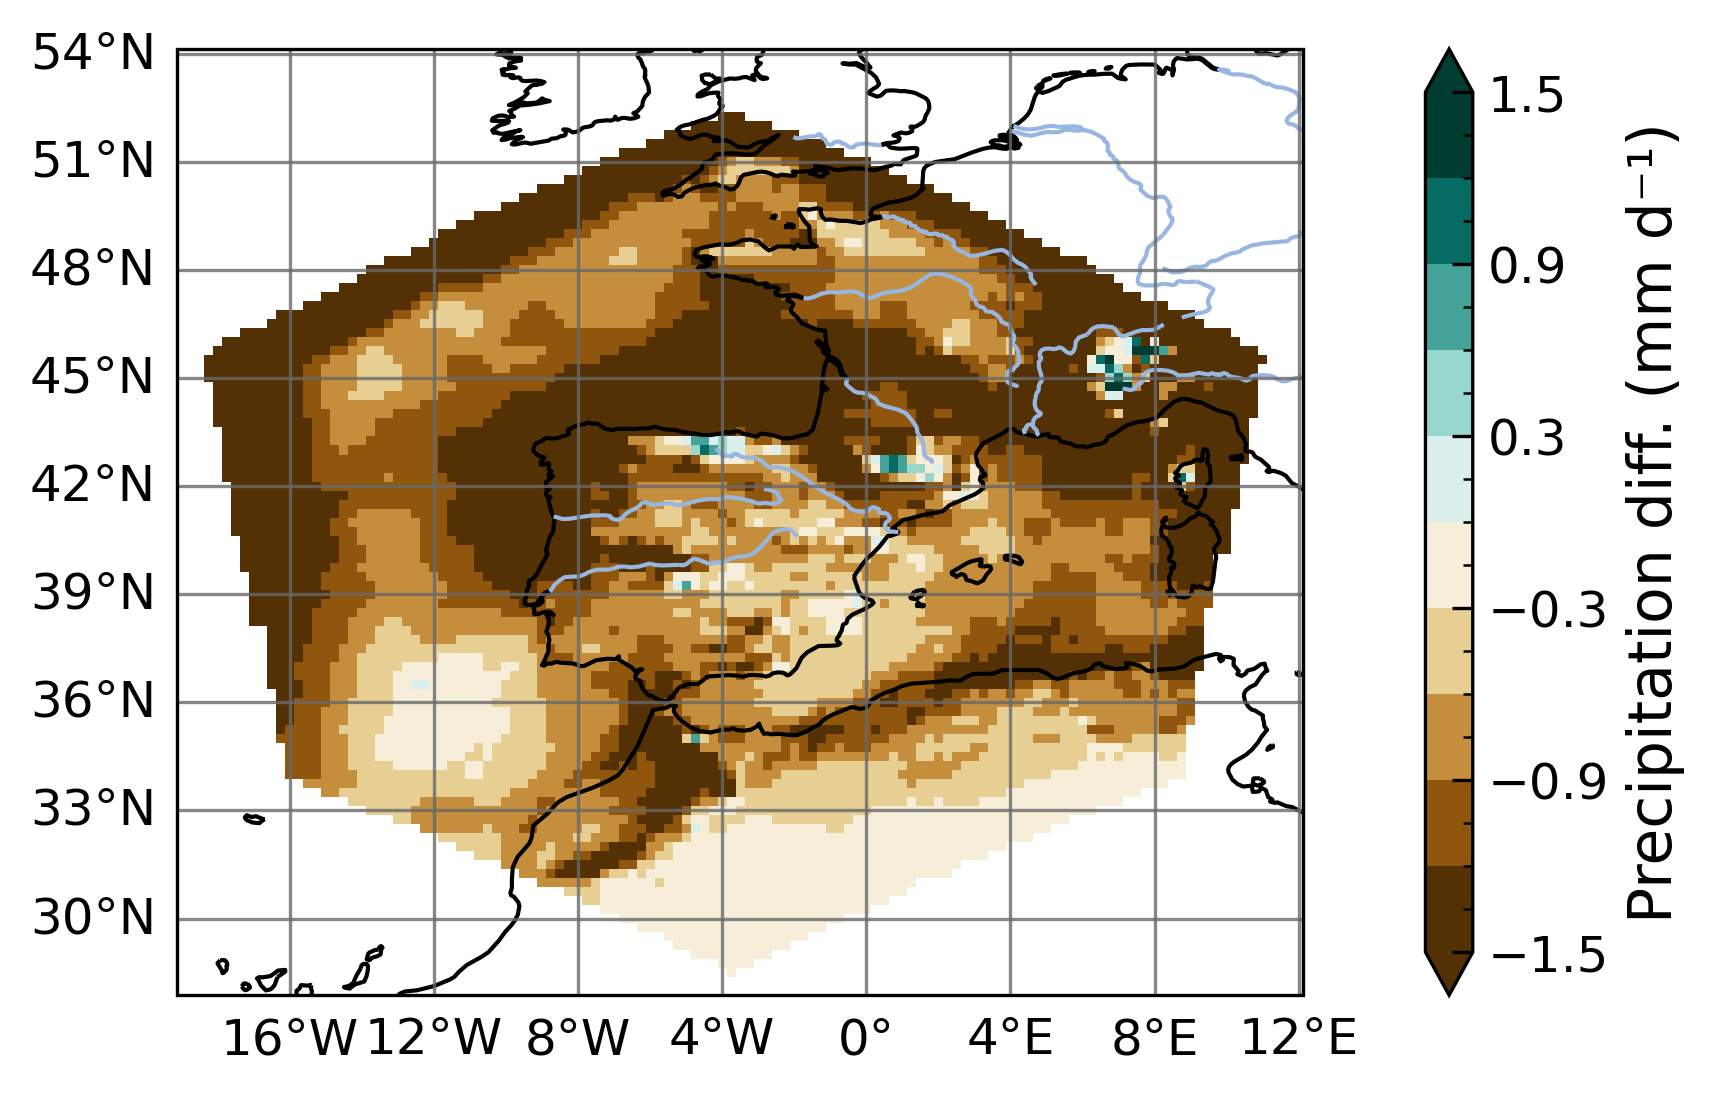
\includegraphics[width=\textwidth]{images/chap4/forcing_sampling_freq/diff_map_precip_lmdz6h_era.png}
        \end{subfigure} \\
        %evap
        \begin{subfigure}[b]{0.33\textwidth}
            \caption{ET bias\\(mm \perday, \forcingoneh)}
            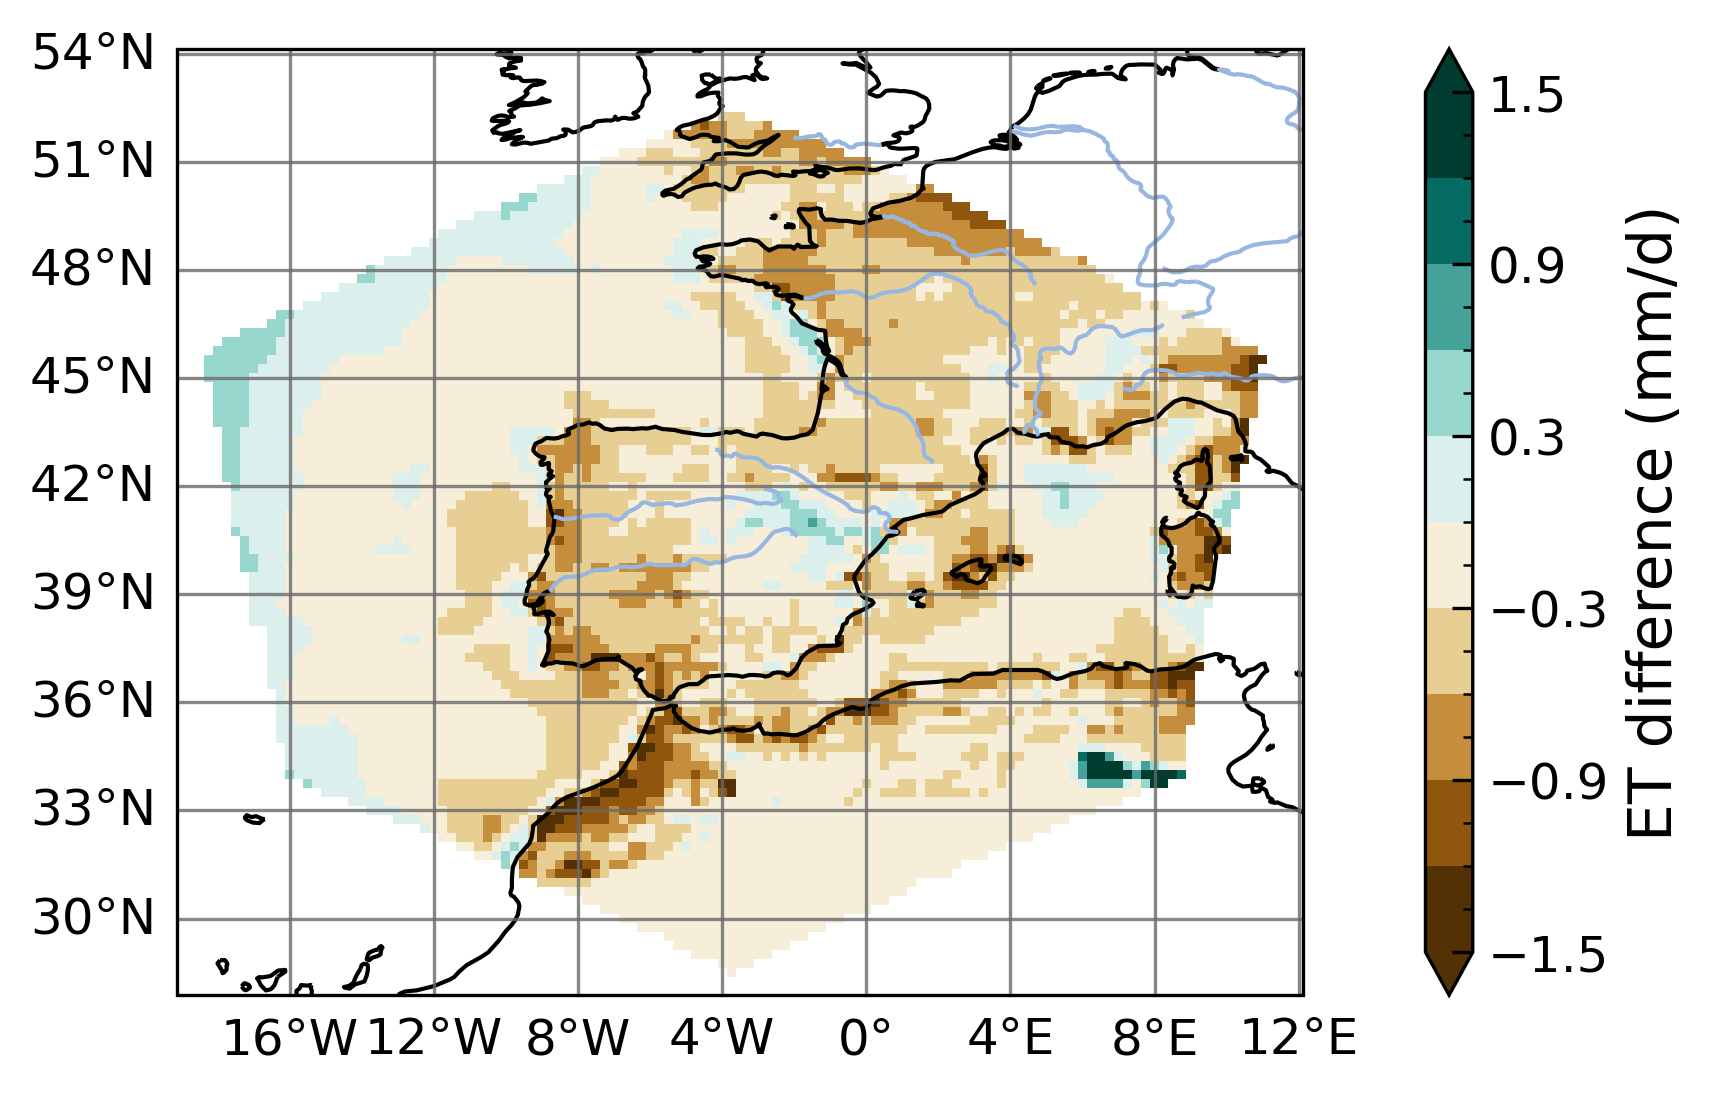
\includegraphics[width=\textwidth]{images/chap4/forcing_sampling_freq/diff_map_evap_lmdz1h_era.png}
        \end{subfigure} &
        \begin{subfigure}[b]{0.33\textwidth}
            \caption{ET bias\\(mm \perday, \forcingsixh)}
            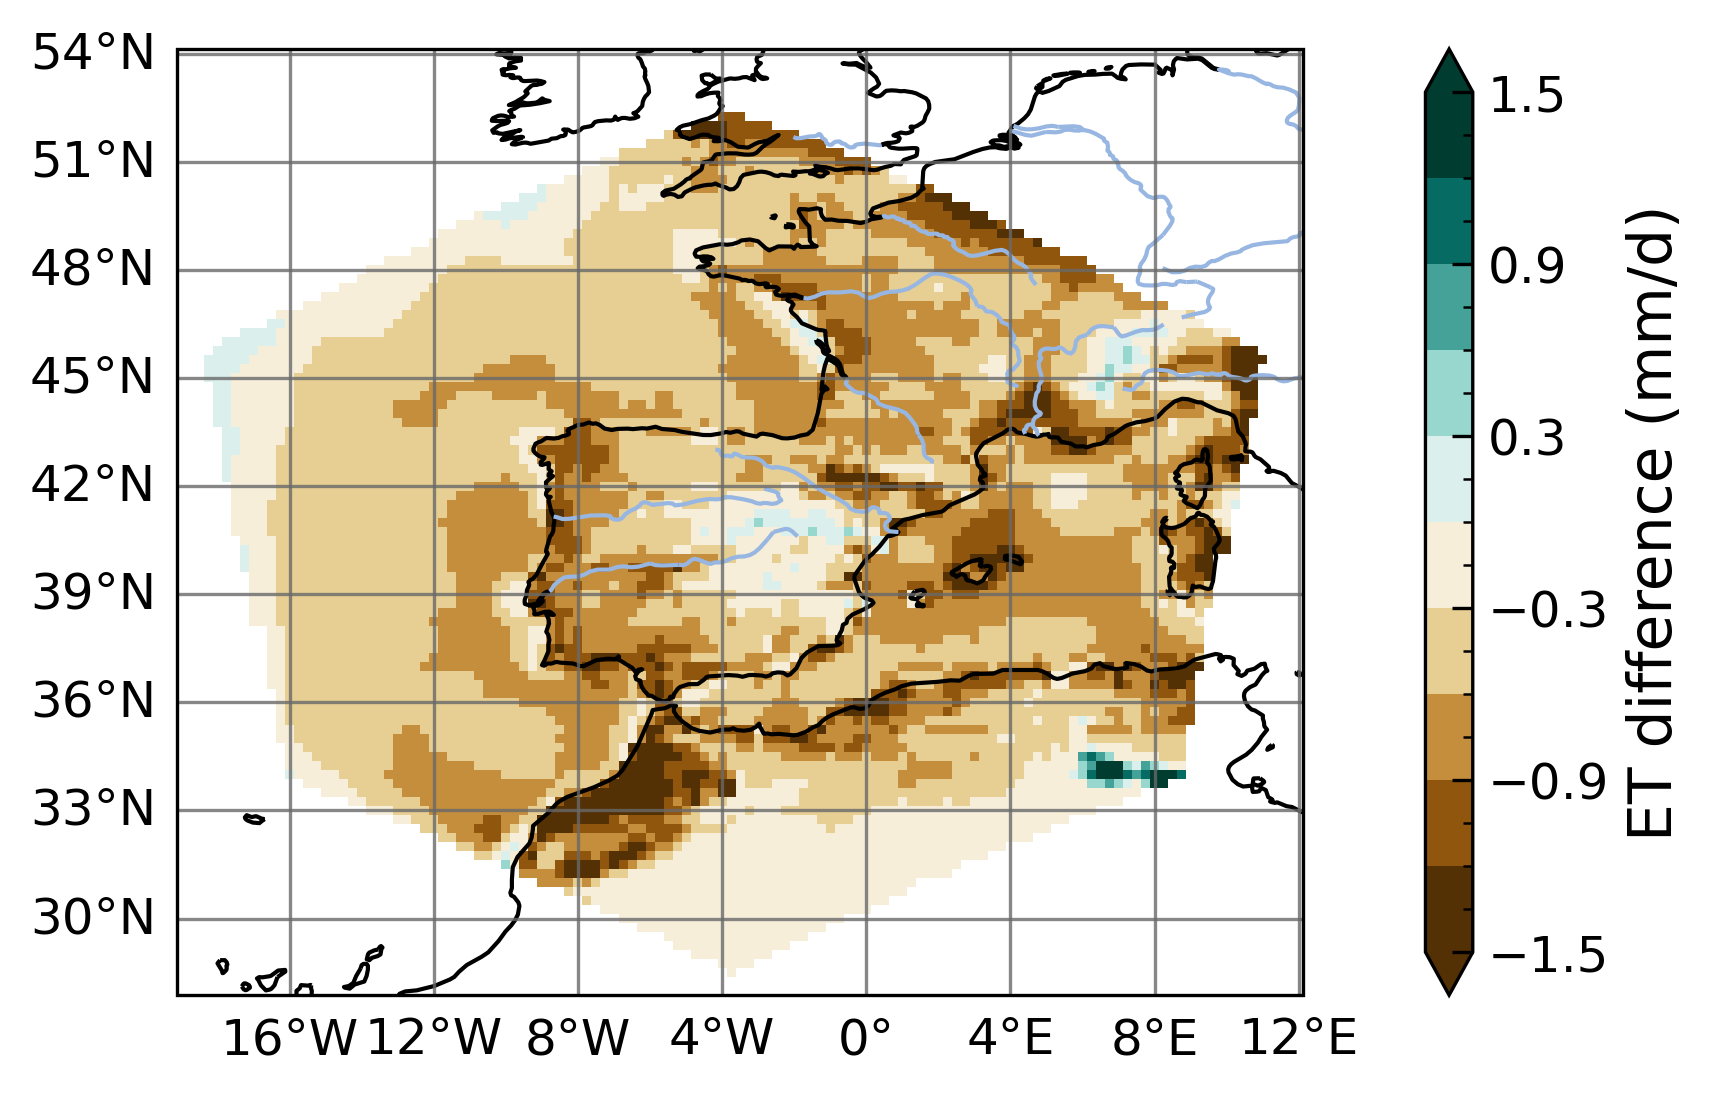
\includegraphics[width=\textwidth]{images/chap4/forcing_sampling_freq/diff_map_evap_lmdz6h_era.png}
        \end{subfigure} \\
        %SWdn
        \begin{subfigure}[b]{0.33\textwidth}
            \caption{Downwelling SW flux bias\\(W \persqm, \forcingoneh)}
            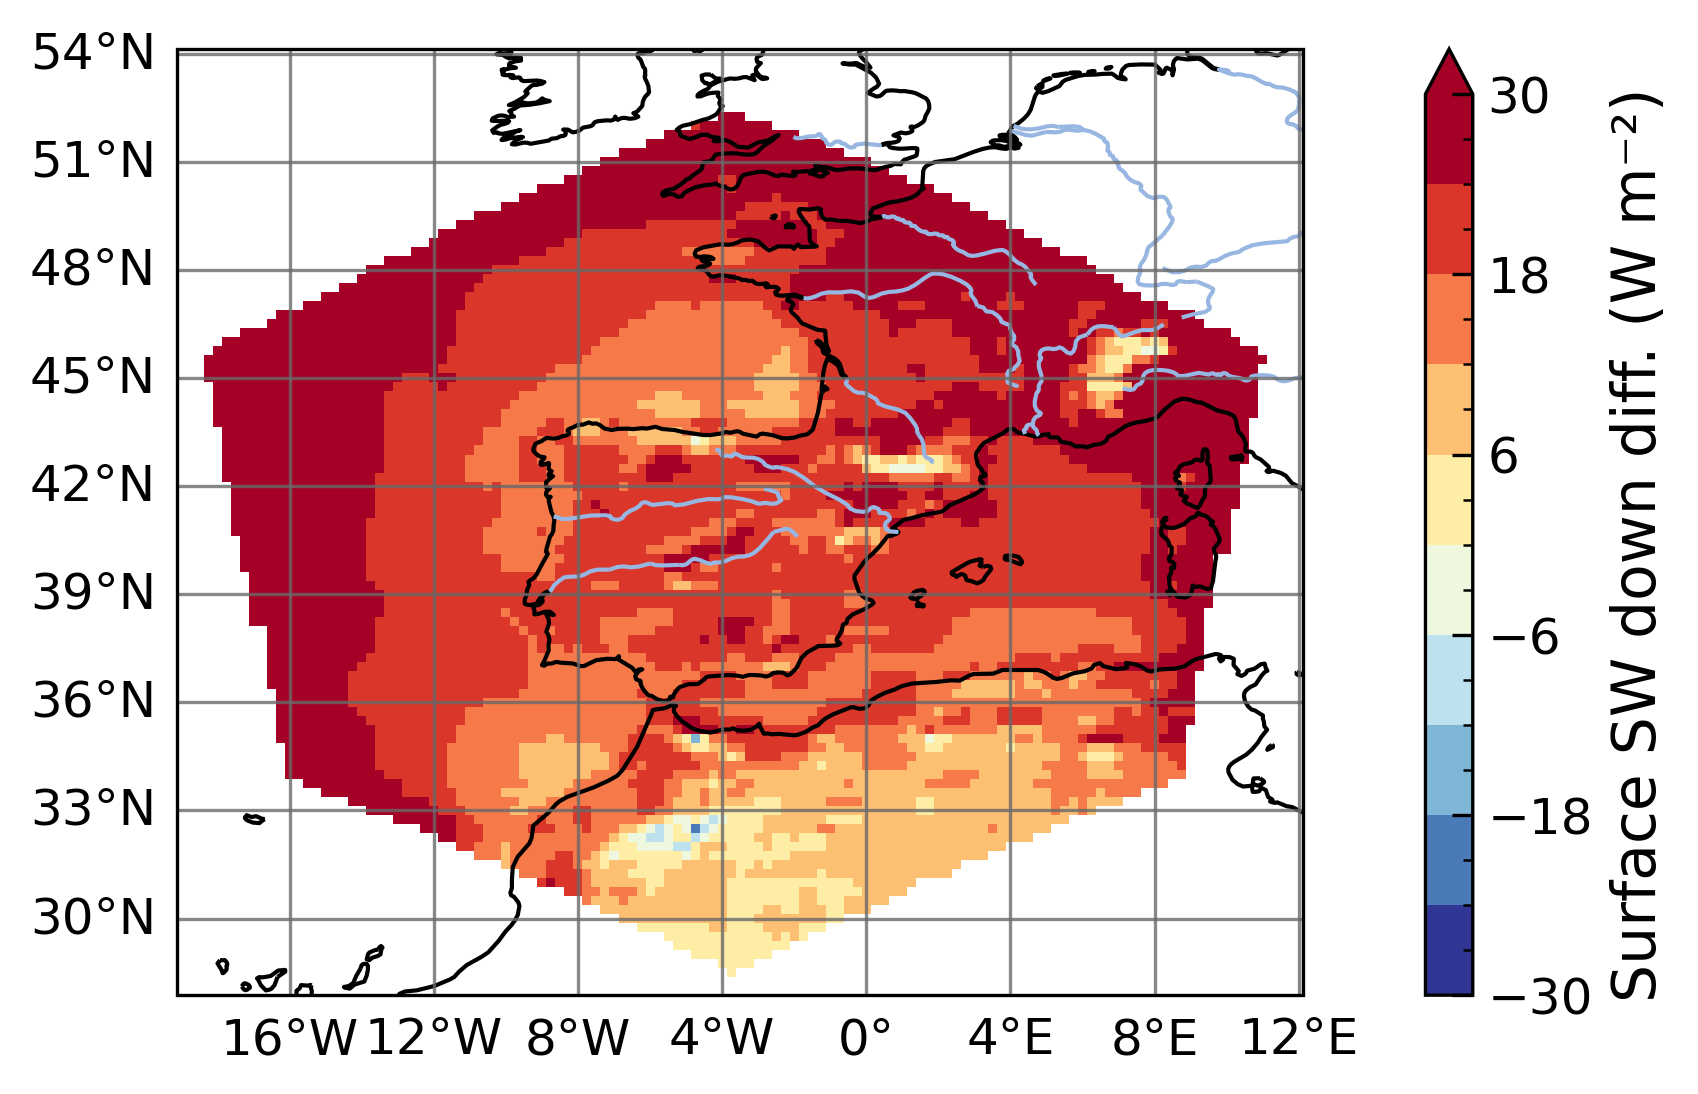
\includegraphics[width=\textwidth]{images/chap4/forcing_sampling_freq/diff_map_SWdnSFC_lmdz1h_era.png}
        \end{subfigure} &
        \begin{subfigure}[b]{0.33\textwidth}
            \caption{Downwelling SW flux bias\\(W \persqm, \forcingsixh)}
            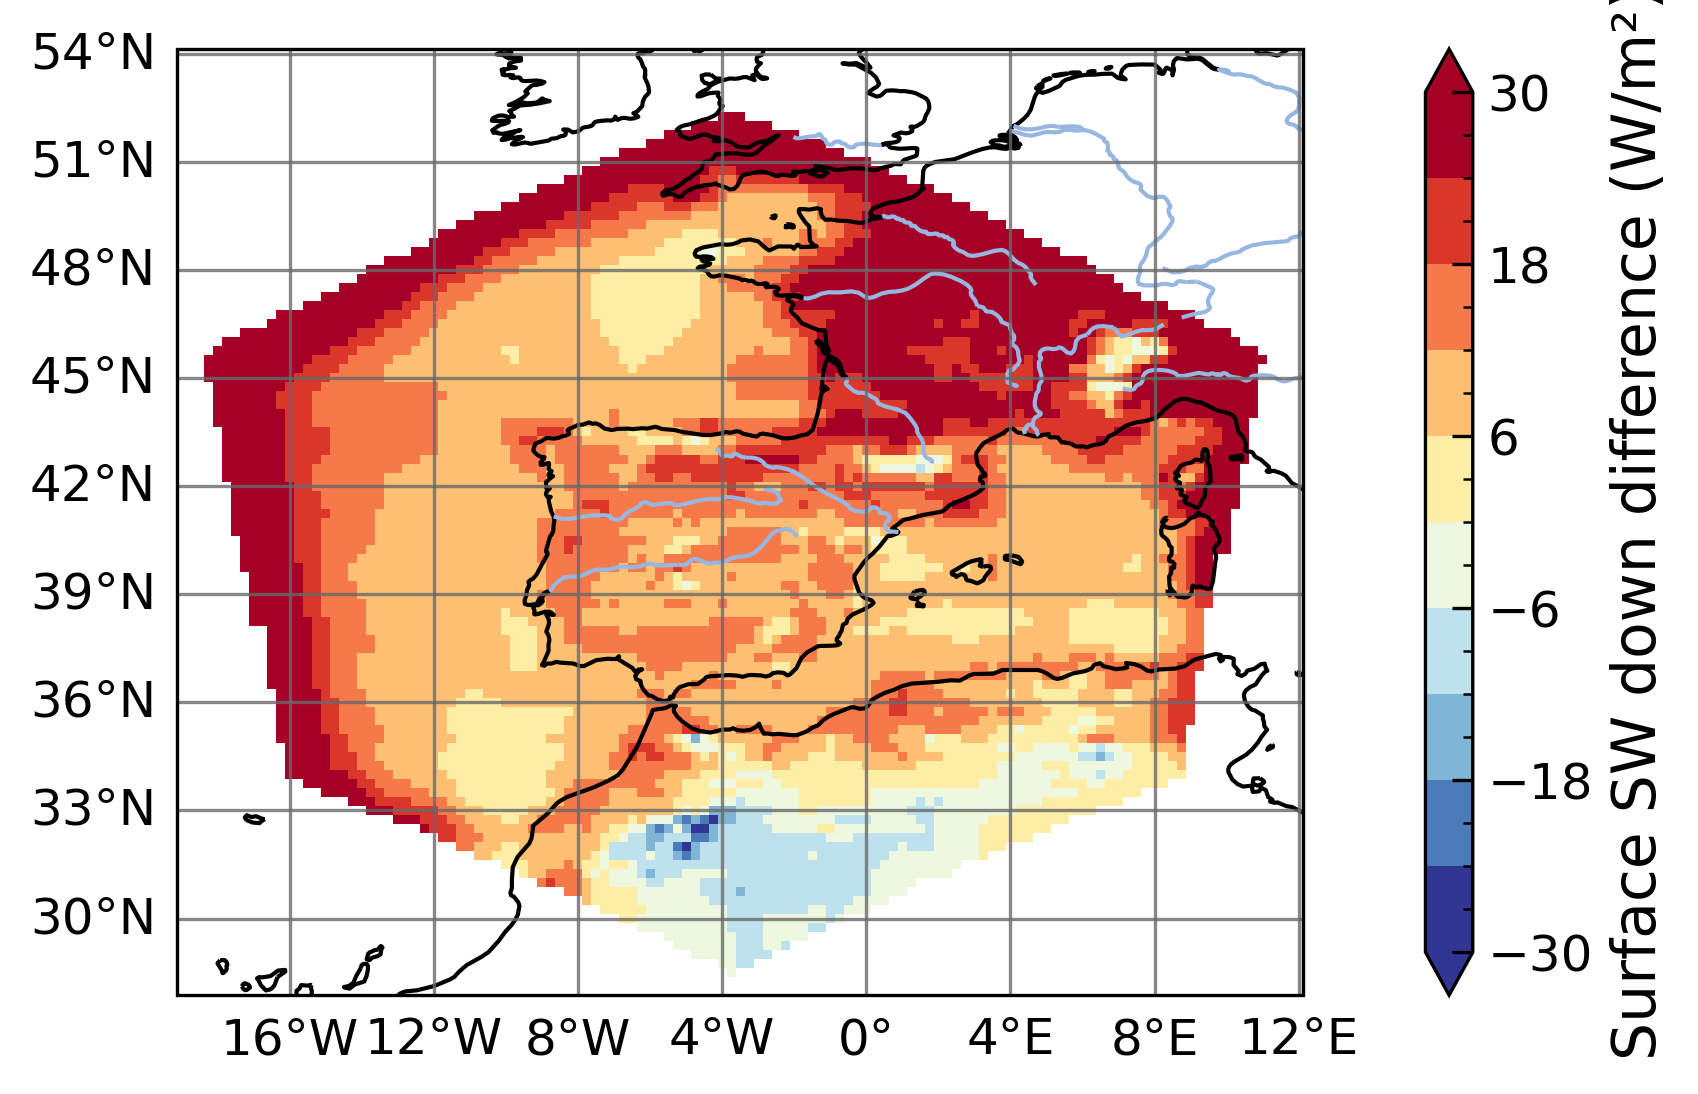
\includegraphics[width=\textwidth]{images/chap4/forcing_sampling_freq/diff_map_SWdnSFC_lmdz6h_era.png}
        \end{subfigure}\\
        %LWdn
        \begin{subfigure}[b]{0.33\textwidth}
            \caption{Downwelling LW flux bias\\(W \persqm, \forcingoneh)}
            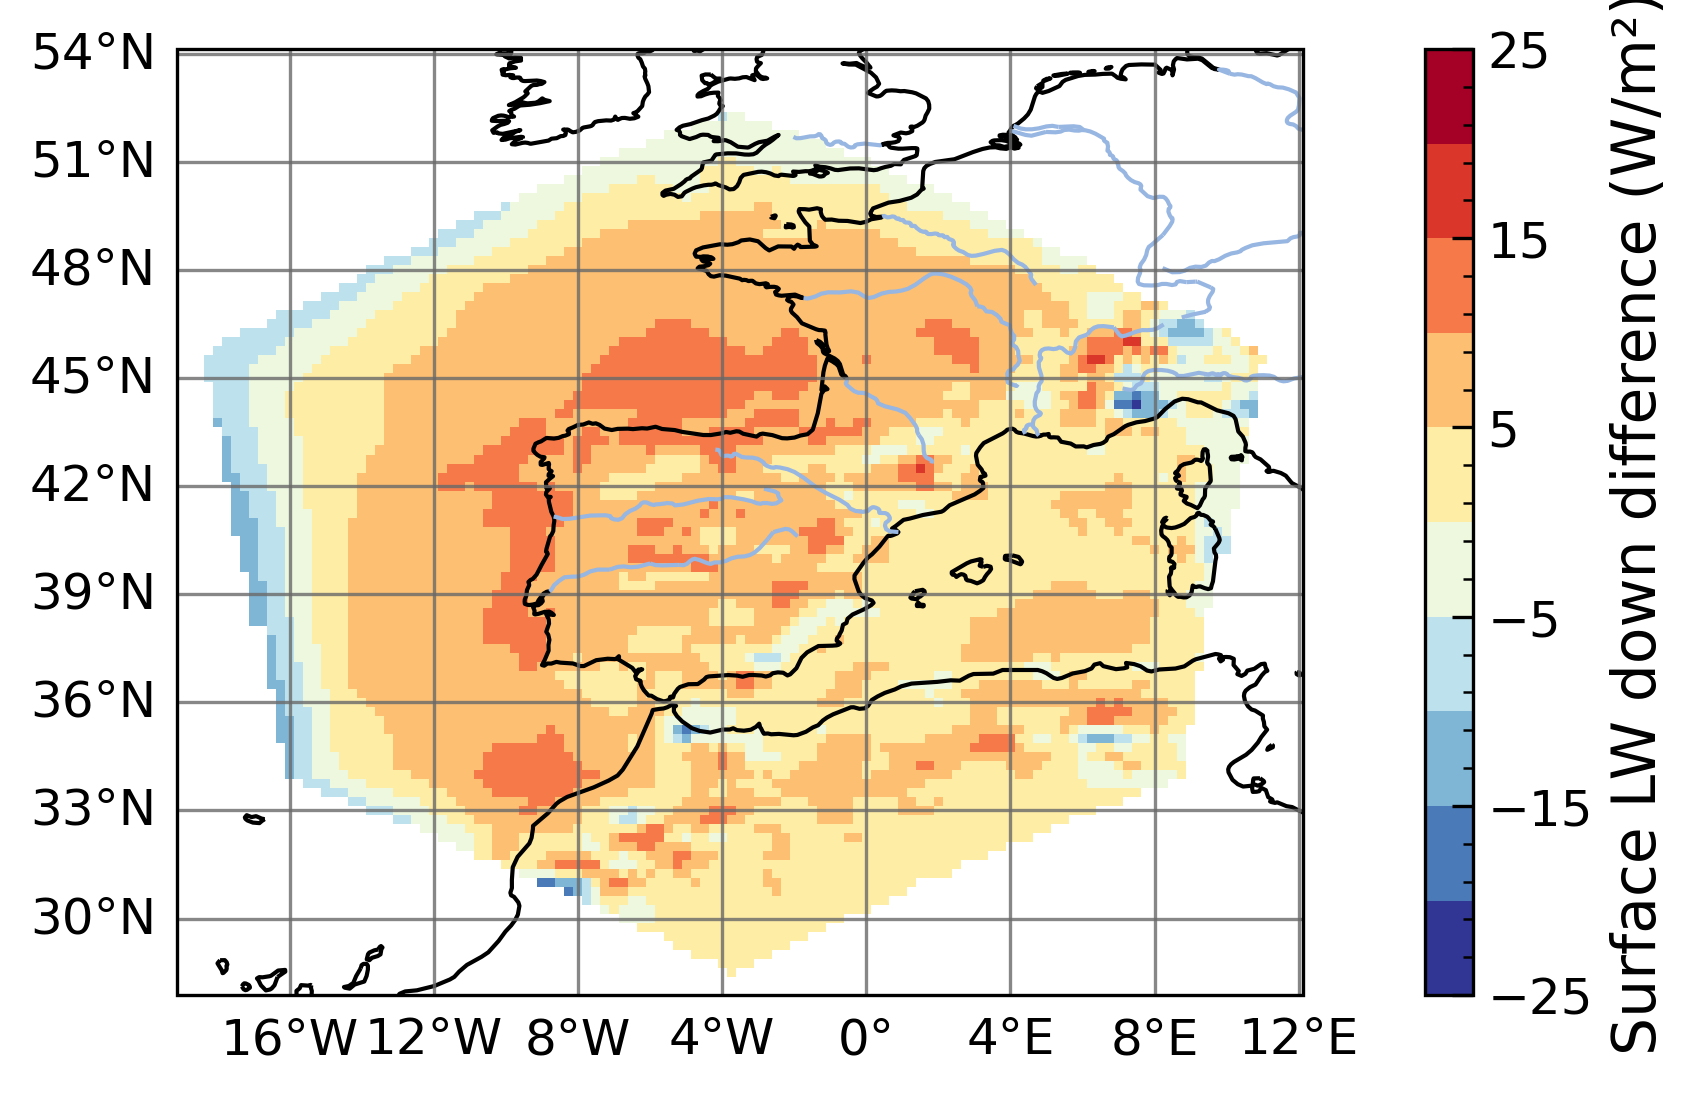
\includegraphics[width=\textwidth]{images/chap4/forcing_sampling_freq/diff_map_LWdnSFC_lmdz1h_era.png}
        \end{subfigure} &
        \begin{subfigure}[b]{0.33\textwidth}
            \caption{Downwelling LW flux bias\\(W \persqm, \forcingsixh)}
            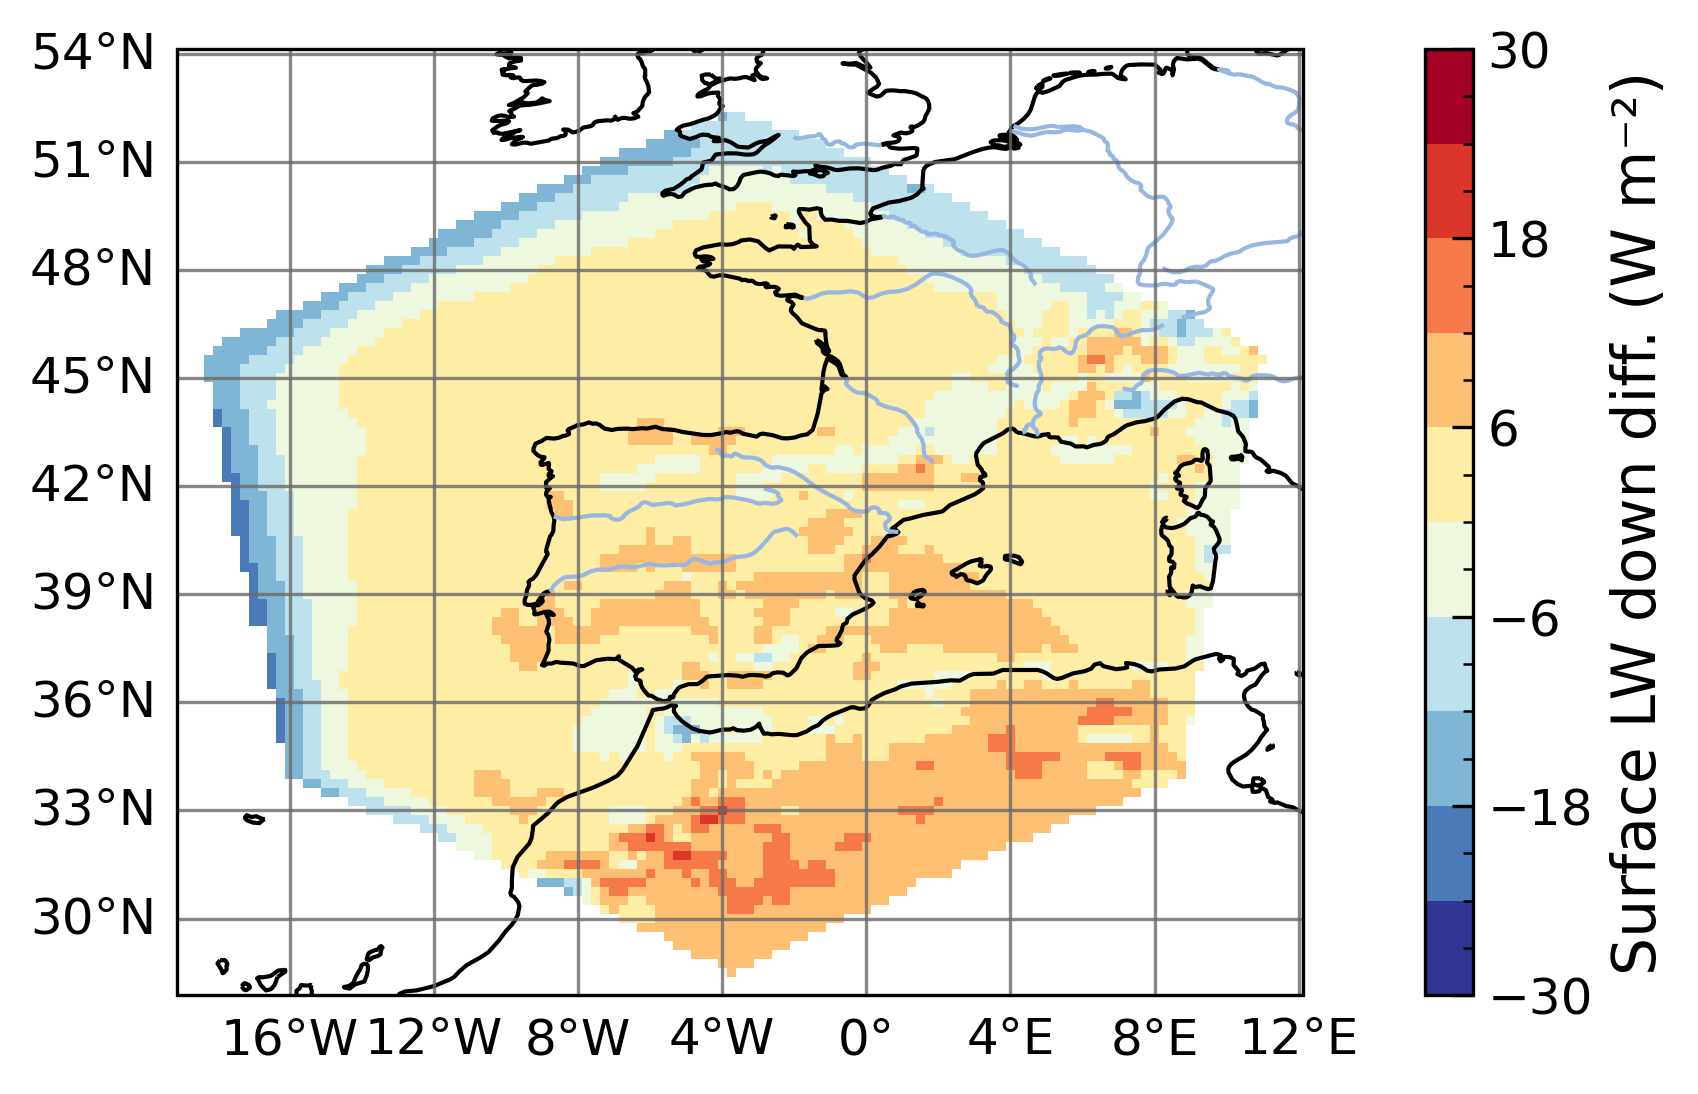
\includegraphics[width=\textwidth]{images/chap4/forcing_sampling_freq/diff_map_LWdnSFC_lmdz6h_era.png}
        \end{subfigure} \\
    \end{tabular}
    \caption{Biases of precipitation, evapotranspiration, and downwelling radiative fluxes for the two simulations, with hourly and 6-hourly forcing data, compared to ERA (2013).}
    \label{fig:forcing_sampling_freq_ERA_diff_maps}
\end{figure}

For practical reasons, running long LAM simulations or simulations under future climate using simulation outputs in CMIP format as a source for the forcing data would require to use a forcing file with a 6-hours sampling frequency rather than one hour. 
Although the other simulations used in this manuscript were eventually all run with hourly forcing data, an experiment was conducted to assess the effects of the sampling frequency of the forcing file on the LAM. 
The results presented here compare two simulations with the intermediate domain size and lateral boundary conditions obtained from ERA5, with hourly data (\forcingoneh) and with 6-hourly data (\forcingsixh). Technical issues were encountered when trying to run with 6-hourly forcing data and only the year 2013 could be run without problems. Therefore, this single year was simulated ten times in a row in each simulation setup, constituting two small simulation ensembles.

\hfill

First, it is clear that the biases in the transition zone identified in Section \ref{sec:domain_size} for downwelling radiative fluxes are strengthened in \forcingsixh (Fig. \ref{fig:forcing_sampling_freq_ERA_diff_maps}f, h). 
Compared to \forcingoneh, shortwave flux is increased and longwave flux is decrease over the whole domain, and are associated to a reduced cloud cover (see Fig. \ref{fig:forcing_sampling_freq_ERA_diff_maps_appendix} in the appendix).
In \forcingsixh, precipitation remains near-zero in the transition zone, and the bias seems confined to the edges (Fig. \ref{fig:forcing_sampling_freq_ERA_diff_maps}b). However, precipitation is largely underestimated in the central part of the domain, including continental areas in the north-west of the Peninsula, the Ebro valley, and near the Gibraltar straight. Considering the structure of the bias, this does not seem to be a direct consequence of the inconsistencies in the transition zone, but might still be an indirect consequence of the discrepancies between the physics used by ERA5 and LMDZ.
The underestimation of ET is generally strengthened in \forcingsixh than in \forcingoneh, which is not very well correlated with the changes found for radiative fluxes over the sea (Fig. \ref{fig:forcing_sampling_freq_ERA_diff_maps}d). This might be due to more complex feedback loops involving ET, atmospheric humidity, cloud cover, and therefore surface radiation, but it was not investigated further due to the scope of this study.
Over land, the underestimations of ET compare to ERA5 reflect those of precipitations but only to some extent, mostly in the Ebro valley and the western part of the domain.

On average over the Iberian Peninsula, the seasonal cycle of precipitation and ET have similar characteristics in both simulations, but \forcingsixh presents less precipitation all year, leading to a stronger underestimation in summer, autumn and winter compared to GPCC (Fig. \ref{fig:forcing_sampling_freq_SC}a). This lower amount of precipitation is logically associated to a lower ET in the seasons where it is limited by available soil moisture, which also increases the underestimation compared to GLEAM data (Fig. \ref{fig:forcing_sampling_freq_SC}b). 

%figure : SC of precip and evap with GLEAM and GPCC
\begin{figure}[htbp]
    \centering
    %precip
    \begin{subfigure}[b]{0.49\textwidth}
        \caption{Seasonal cycle of precipitation (2013)}
        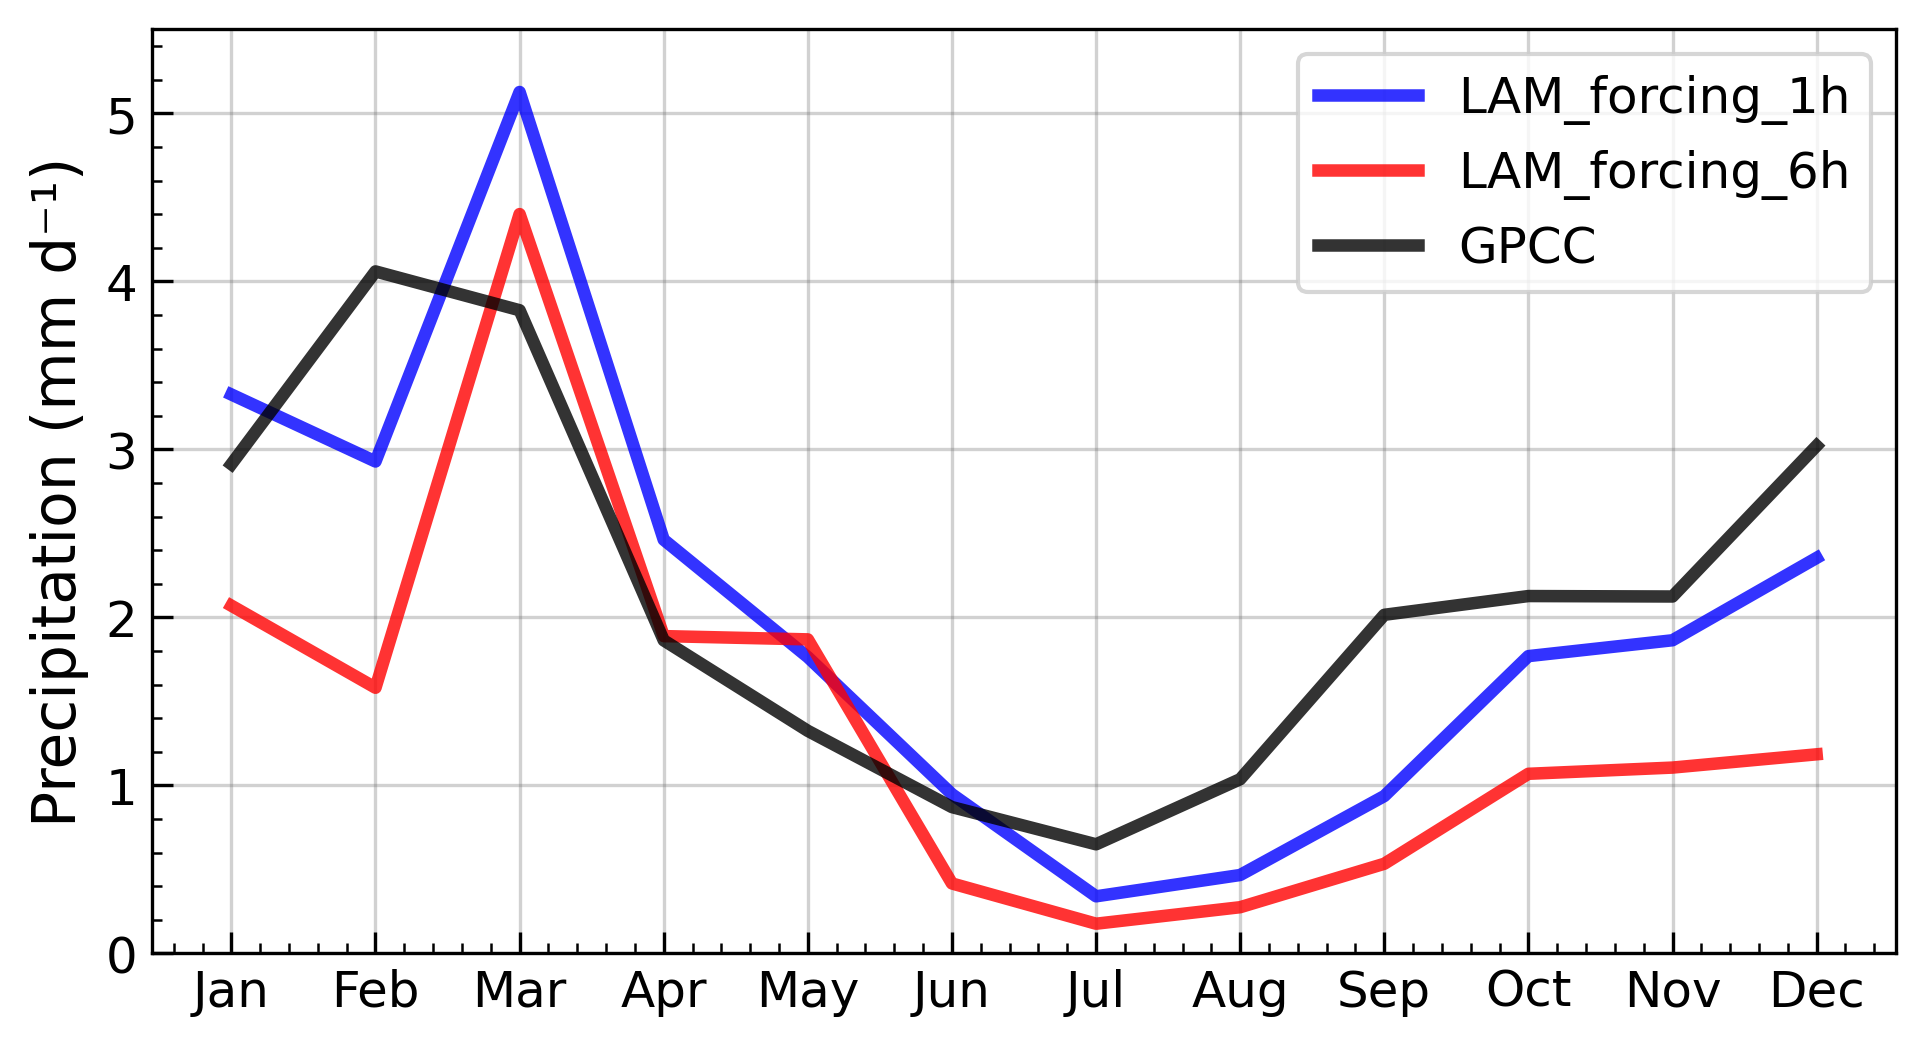
\includegraphics[width=\textwidth]{images/chap4/forcing_sampling_freq/IP_seasonal_cycle_precip.png}
    \end{subfigure}
    \begin{subfigure}[b]{0.49\textwidth}
        \caption{Seasonal cycle of ET (2013)}
        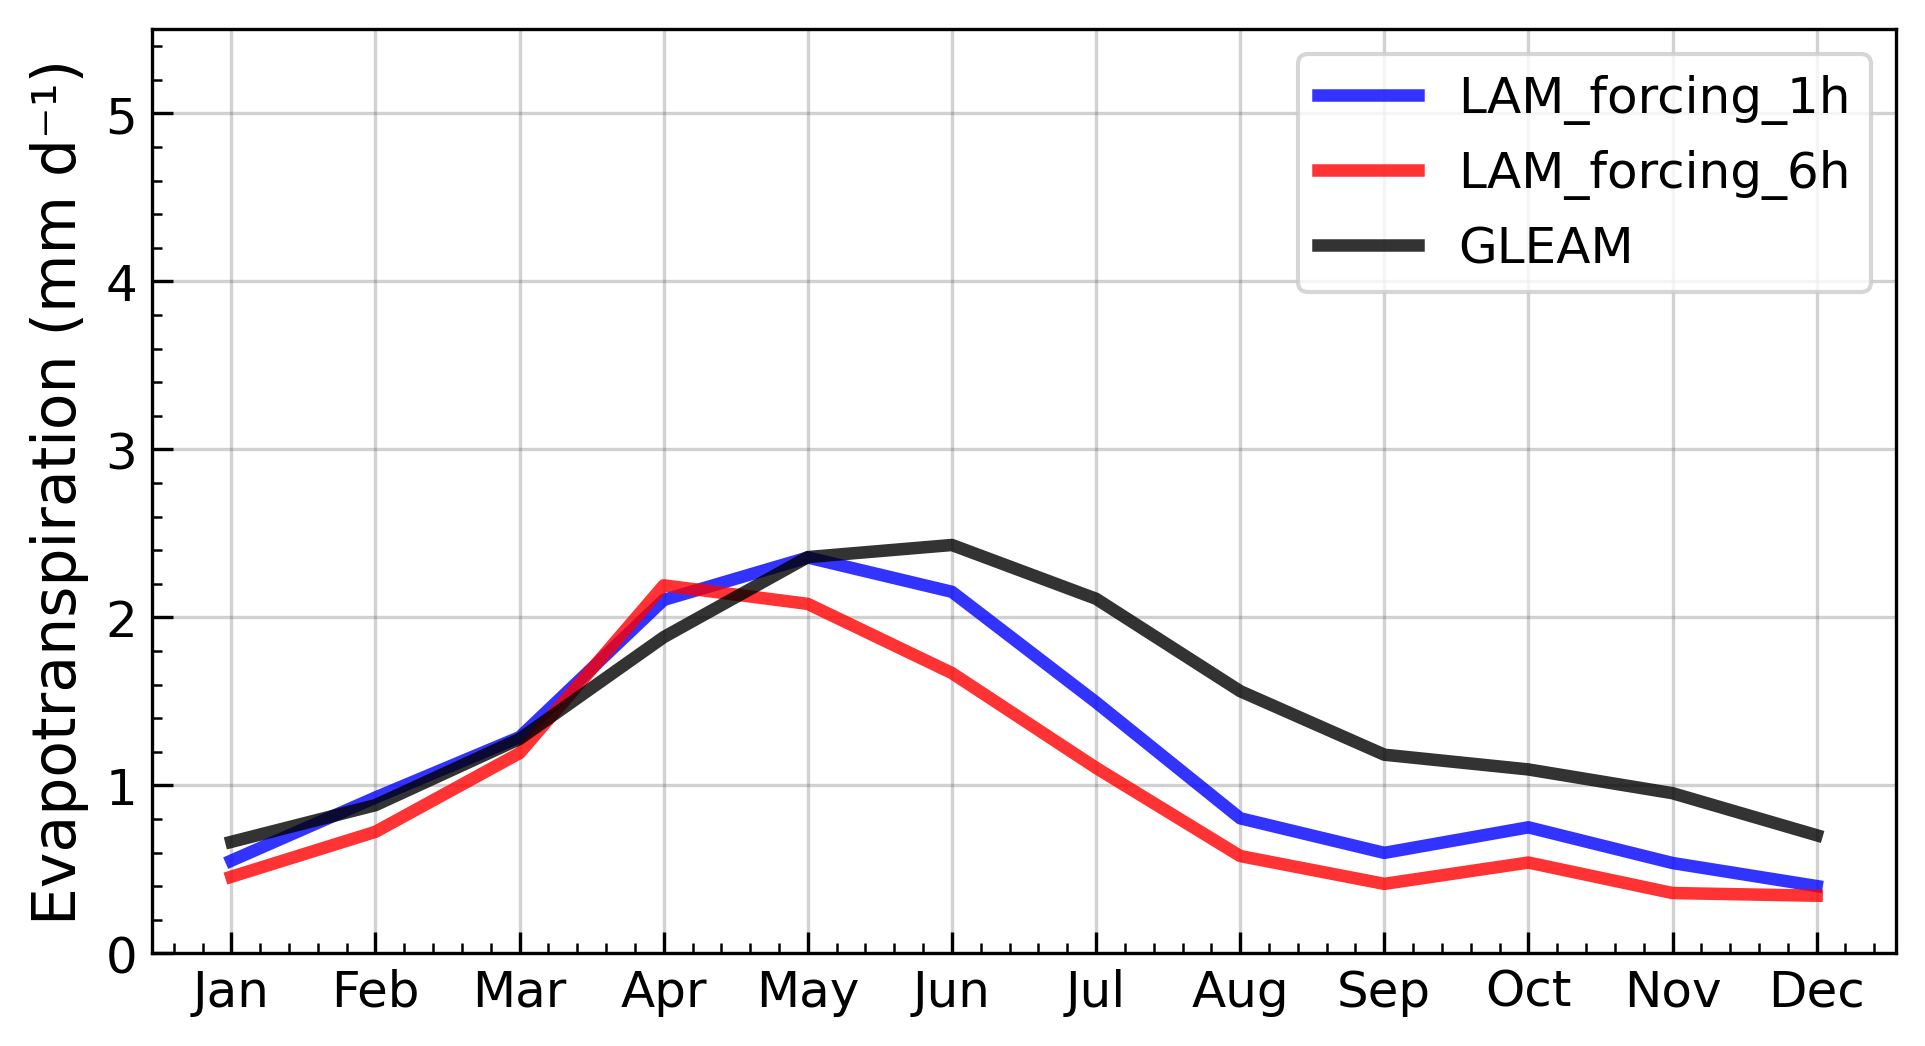
\includegraphics[width=\textwidth]{images/chap4/forcing_sampling_freq/IP_seasonal_cycle_evap.png}
    \end{subfigure}
    \caption{Mean seasonal cycle of precipitation and evapotranspiration, on average over the Iberian Peninsula, for the LAM forced with hourly (blue) and 6-hourly (red) forcing data, and the GPCC and GLEAM products (2013).}
    \label{fig:forcing_sampling_freq_SC}
\end{figure}

Although this study only focused on a single year, it revealed that the LAM is sensitive to the sampling frequency of the ERA5 forcing file. 
To understand it, one must remember that a lower forcing file sampling frequency does not mean the model is less constrained: variables are still nudged at every time step of the dynamics (30 seconds), with the same intensity. However, with a lower sampling frequency, the diurnal cycle is not as well described in the forcing data, as illustrated in Fig. \ref{fig:diurnal_cycle_sampling}. 
For the variables that follow a marked diurnal cycle conditioned by radiative fluxes or the mixing of the lower atmosphere, the inconsistencies between the LMDZ physics and the ERA5 forcing data can therefore be increased and lead to more intense biases. 

\begin{figure}[ht]
    \centering
    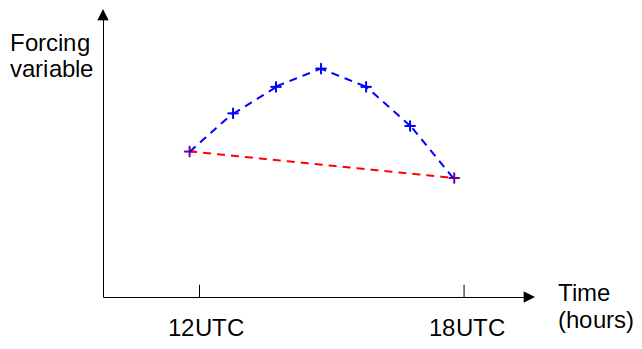
\includegraphics[width=0.5\textwidth]{images/chap4/forcing_sampling_freq/sampling_freq_diurnal_cycle.png}    
    \caption{Illustration of the differences in diurnal cycle sampling using hourly (blue) or 6-hourly (red) forcing data. Adapted from Mariame Maiga's internship defence.
    \label{fig:diurnal_cycle_sampling}}
\end{figure}

\section{Chapter conclusions}

To identify an appropriate simulation setup for the study of the impacts of irrigation, the sensitivities of the LAM to the size of the domain and to the choice of lateral forcing (both its source and sampling frequency) were analysed. They revealed an inconsistent behaviour of the LAM in the transition zone when forced by ERA5 data, in particular unexpectedly low precipitation and cloud cover. These biases were attributed to discrepancies between the physics used to produce the ERA5 reanalysis and the LMDZ physics, which can keep the large-scale condensation scheme from forming clouds and precipitation properly.
This inconsistent behaviour in the transition zone was found to also have impacts in the central part of the domain, including over the Iberian Peninsula. Using larger domains does not make these inconsistencies disappear but limits their direct influence over the Peninsula since the transition zone is further away. More generally, when using lateral boundary conditions from ERA5, a dry bias (on precipitation and continental ET) still affects the whole simulation domain in all the configurations used, which might be a more indirect consequence of these discrepancies.

A simulation forced with outputs from a global ICOLMDZOR simulation was compared to the initial setup with forcing data from ERA5 and showed large improvements in the consistency of the model in the transition zone and a reduction of the precipitation and ET biases over the whole domain.
These findings confirmed that the model is sensitive to the source of the forcing data, and identified a possibly better forcing source for future studies with the LAM. However, with this setup, some inherent biases of the ICOLMDZOR model appear in the central zone (\textit{e.g.} excessive winter precipitation in mountains), which partly limits the improvements in performance over the Iberian Peninsula. 

Sensitivity experiments to look into the impact of the forcing file sampling frequency were also conducted. They showed that using 6-hourly ERA5 data for the lateral forcing instead of hourly data increases the biases of the radiative fluxes in the transition zone and the central free zone. Precipitation and ET are also affected although it remains difficult to interpret the structure of the biases and possible links to the inconsistencies of the transition zone.
Over the Iberian Peninsula, the performance is partly degraded for precipitation and ET, as the LAM displays an increased dry bias when using 6-hourly data. 

However, the limitations identified in this simplified evaluation do not discard LAM simulations with 6-hourly forcing data as a viable option for regional climate modelling.
As a reminder, the setup used for this analysis of the sampling frequency was limited to one simulation year (repeated multiple times), and different conclusions might be obtained in other experiments over a longer period, or with a different forcing source that does not generate such strong inconsistencies in the transition zone.
In his internship report, \citet{conesa2022} had analysed the sensitivity of the LAM (in an idealised setup with simplified physics) and found that hourly data performed very similarly to higher sampling frequency (down to 5 mn), that errors became significant for 3-hourly data but remained largely acceptable for 6-hourly data, but that performance was further degraded for 12-hourly data.
Since \citet{denis_sensitivity_2003}, 6-hourly lateral boundary conditions have generally been considered as a good compromise that can properly simulate regional climate \citep[enabling similar performance to 3-hourly data,][]{dimitrijevic_validation_2005}, while limiting the need for large data storage and high-frequency forcing data generation.
In practice, although this analysis was conducted with the idea that 6-hourly forcing data could be used for future climate simulations, this option was eventually discarded for technical reasons (frequent unexplained model crashes) and all simulations used in the rest of this manuscript were run using hourly forcing data.

\hfill

To summarise, despite several simplifications due to technical and time constraints in the context of Mariame Maiga's internship, several dependences of the ICOLMDZOR LAM on the choice of the domain and forcing data were identified. This work is of high interest for the IPSL modelling community since the LAM is a recent tool, still in development, that is expected to be used in more and more regional modelling and parametrization development studies.
The results would benefit from further consolidation with longer simulations to enable statistical analyses on climatic time scales, and from a study of mixed effects of domain size, forcing source and sampling frequency to identify the most appropriate setups for future regional climate simulations with the LAM.
The influence of the resolution of the forcing could also be investigated as is has long been identified as an important sensitivity of regional climate models \citep{leduc_regional_2009}. In this regard, the zooming capability of the global ICOLMDZOR model might prove very useful to generate forcings that match the resolution of the LAM over the transition zone. Additional research directions to increase the understanding and reliability of the LAM are detailed in Section \ref{sec:lam_perspectives}.